% Packages and formatting

\documentclass[12pt,epsfig]{article}
\usepackage{graphicx,subfigure,amsmath,latexsym,amssymb, mathtools}
\usepackage{epsfig,pdfpages,float,changepage}
\usepackage{longtable}
\usepackage{rotating}
\usepackage{braket}
\usepackage{tikz}
\usepackage{authblk}
\usepackage{esvect}
\usepackage{appendix}
\usepackage{xcolor}
%\usepackage{natbib}
\usepackage[natbibapa]{apacite}
%\usepackage{apalike}
\usepackage[width=1.3\textwidth]{caption}

\newcommand{\change}[1]{\textcolor{black}{#1}}
\newcommand{\changed}[1]{\textcolor{black}{#1}}

\DeclareMathOperator*{\argmax}{arg\,max}
\DeclareMathOperator*{\argmin}{arg\,min}

\usepackage[margin=1.25in]{geometry}

\providecommand{\keywords}[1]
{
  \small	
  \textbf{\textit{Keywords---}} #1
}

\parindent=0.5in

% Sample size commands for revision
\newcommand{\numsubjects}{\changed{n}}%Originally {k}
\newcommand{\testlength}{\changed{k}}%Originally {n}

\linespread{1}

\begin{document}


%\linespacing{1}



%\title{Some Generalizations of Kuder-Richardson Formulas 20 and 21 within the Natural Exponential Family}
\title{KR-20 and KR-21 for some non-dichotomous data (It's not just Cronbach's alpha)}
\author{Robert C. Foster}
\affil{Bettis Atomic Power Laboratory}
\date{}
\maketitle

%\begin{center}
%ACCEPTED FOR PUBLICATION IN \emph{EDUCATIONAL AND PSYCHOLOGICAL MEASUREMENT}
%\end{center}

\begin{abstract}
This paper presents some equivalent forms of the common Kuder-Richardson Formula 21 and 20 estimators for non-dichotomous data belonging to certain other exponential families, such as Poisson count data, exponential data, or geometric counts of trials until failure. Using the generalized framework of \cite{Foster2020}, an equation for the reliability for a subset of the natural exponential family have quadratic variance function is derived for known population parameters, and both formulas are shown to be different plug-in estimators of this quantity. The equivalent Kuder-Richards formulas 20 and 21 are given for six different natural exponential families, and these match earlier derivations in the case of binomial and Poisson data. Simulations show performance exceeding that of Cronbach's alpha in terms of root mean squared error when the formula matching the correct exponential family is used, and a discussion of Jensen's inequality suggests explanations for peculiarities of the bias and standard error of the simulations across the different exponential families.
\end{abstract}

\keywords{Reliability, KR-20, KR-21, Cronbach's Alpha, Exponential Families}

%\newpage

\newpage

%\tableofcontents % Uncomment if you want a table of contents
% \newpage

% BODY OF PAPER


\section{Introduction}

Formulas 20 and 21 of \cite{Kuder1937}, abbreviated throughout this paper as KR20 and KR21, are some of the earliest and most well-known formulas in assessing reliability of a test. For dichotomous data, the formulas are given by

\begin{gather*}
KR20 = \dfrac{\testlength}{\testlength-1} \left(1 -  \dfrac{\sum_{j = 1}^{\testlength} p_j (1 - p_j)}{\sigma^2_X}\right)\\
KR21 = \dfrac{\testlength}{\testlength-1} \left( 1 - \dfrac{\testlength \bar{p}(1 - \bar{p})}{\sigma^2_X}\right)
\end{gather*} 

\noindent where $\testlength$ is the test length, $\sigma^2_X$ is the variance of sum test scores, $p_j$ is the proportion of correct responses to test item $j$, and $\bar{p}$ is the average correct response over all items. The most common estimator of reliability, Cronbach's alpha, is often seen as a general version of KR20 \citep{Cronbach1951}.  Beyond Cronbach's alpha, there does not seem to have been many attempts to determine equivalent variants of KR20 and KR21 to specific types non-dichotomous data, such as count data. \cite{Allison1978} derived a KR21 equivalent for Poisson distributed data, but most have stuck to Cronbach's alpha as a general estimator of reliability. % For general dichotomous data, \cite{Webster1960} derived a formula attempting to extend KR21, and which is equal to the earlier generalized reliability coefficient of \cite{Horst1949}.

\changed{The topic of reliability estimation, and Cronbach's alpha in particular, has been a subject of much recent debate within the psychometric literature. Alpha has been criticized as having assumptions which are not realistic in practice \citep{Schmitt1996,Sijtsma2009, Mcneish2017}.  Criticisms have focused on alpha's assumptions of tau equivalence and uncorrelated errors. \cite{Mcneish2017} claims that normality is an assumption of Cronbach's alpha, but \cite{Raykov2019} rebut that no assumptions of normality are made in the derivation of alpha and consistency as an estimator does not depend on an assumption of normality. However, \cite{Zumbo1999} notes that though the classical test theory derivation of alpha makes no assumptions of normality, estimators of alpha often do, in agreement with \cite{Bay1973} who noted in his time that early derivations of statistical properties of estimators such as Cronbach's alpha and KR20 as in \cite{Feldt1965} were developed using an ANOVA model which includes an assumption of normality. More recent research in \cite{Zyl2000} on the sampling distribution of cronbach's alpha using maximum likelihood techniques also assumes normality,  though nonparametric methods have been developed for psychometric calculations using techniques like the bootstrap as in \cite{Raykov1998}. The statistical properties of alpha and other estimators have been little explored outside of these assumptions of normality, with simulation studies in \cite{Sheng2012} and \cite{Zimmerman1993}. Beyond classical test theory, \cite{Geldhof2014} explicitly state that non-normal data is a limitation for reliability estimation in a multilevel confirmatory factor analysis framework As \cite{Zinbarg2006} note, properties of alternatives to Cronbach's alpha based on a factor analysis are not well known under non-normality, despite most psychological data being non-normal. It is clear that there is a need for analysis of reliability for non-normal data.}

The purpose of this paper is to \changed{make a contribution towards the analysis of reliability under non-normality by reversing direction from Cronbach's alpha once again to} derive formulas to estimate test reliability in special cases -- to find equivalent forms of KR20 and KR21 which can be used to assess reliability of tests for specific types of non-dichotomous data. \changed{For example, chapter 21 of \cite{Lord1968}, discussing the work of \cite{Rasch1960}, notes that the number of an examinee's misreadings in an oral reading test may be modeled as a Poisson random variable. If the response of interest were instead the time between misreadings, an exponential distribution would then be appropriate. \cite{Meredith1971} also showed that a Poisson process is appropriate for tests of speed, and noted that under certain assumptions the distributions of observed scores ought to be negatively binomial distributed.} The key idea is this: KR20 and KR21 can be seen as a specific version of an estimator for reliability for Bernoulli distributed item responses where the mean-variance relationship of the Bernoulli distribution is exploited for variance calculations rather than using standard sample variances. Other exponential family distributions also have mean-variance relationships. By working within the generalized framework of \cite{Foster2020} and deriving a formula for reliability in exponential families which uses the mean-variance relationship and which matches traditional KR20 and KR21 in the binomial case, equivalent versions of KR20 and KR21 are obtained for data from other exponential family distributions. The KR20 and KR21 equivalent formulas are shown for when sum test scores can be said to follow one of the six natural exponential family distributions with quadratic variance function (NEF-QVF): the normal, the binomial, the Poisson, the gamma, the negative binomial, or the natural exponential family generated by a convolution of generalized hyperbolic secant functions (NEF-GHS). %Importantly, these estimators are best thought of as statistical estimators of some underlying population quantity.


Section \ref{Sec:Framework} describes the properties of the generalized framework for reliability described in \cite{Foster2020} which form the basis for derivations of the formulas and definition of reliability as parallel-test correlation, and states which assumptions are slightly modified for the purposes of this paper. Section \ref{Sec:Estimators} shows how the mean-variance relationship can be exploited to obtain test reliability and derives the general KR20 and KR21 formulas as estimators of this relationship, giving the formulas for each NEF-QVF distribution. These are shown to match the traditional KR20 and KR21 of \cite{Kuder1937} in the binomial case, and the Poisson KR21 of \cite{Allison1978} in the Poisson case. \changed{The conditions for algebraic equivalence between KR20 and Cronbach's alpha are also discussed.}  Section \ref{Sec:Simulations} performs a simulation study showing that these formulas do appear to converge to the population reliability as the number of subjects and test length increases and comparing the equivalent KR20 and KR21 formulas to Cronbach's alpha and each other in terms of root mean squared error, bias, and standard deviation. Results indicate that when the formulas are used for data following the appropriate exponential family, performance is improved over Cronbach's alpha in terms of RMSE, though whether KR20 or KR21 is superior depends on the variance function of the exponential distribution. A brief discussion of Jensen's inequality indicates a possible explanation for why one formula is superior to another for a given distribution.

%\section{Previous Work} 
%\label{Sec:LitReview}

%Cronbach's alpha of \cite{Cronbach1951} is often describe to as the general version of $KR20$ and $KR21$, intended to apply generally to non-dichotomous data.

%\cite{Lord1968}

%Also of interest are papers which attempt parametric estimation of $KR20$ and $KR21$. Most prominent is the work of paper \cite{Keats1962} which derives $KR21$ as the through the assumption of a binomial-beta model. 

%Is this fucking it? There has to be more.  \cite{Allison1978}

\section{Framework}
\label{Sec:Framework}

This paper follows the generalized framework of \cite{Foster2020}\changed{, where ``generalized'' is used in the same sense of a generalized linear model which may deal with non-normal exponential family data}. A complete theoretical description of the framework is given in \cite{Foster2020}, but this paper will only state without proof elements which are necessary. One major difference is that while the framework of \cite{Foster2020} applies to the entire natural exponential family, this paper focuses only on the members of the exponential family having quadratic variance function \changed{so that the variance is a polynomial function of the mean up to degree two. For example, a Bernoulli distribution with success probability $p$ has mean $p$ and variance $p(1-p) = p - p^2$, so the variance is a quadratic function of the mean.} Such distributions and their properties are extensively described in \cite{Morris1982} and \cite{Morris1983}, which serve as a general reference. Furthermore, while the framework of \cite{Foster2020} allows the test length to vary between subjects, this paper assumes a common test length for all subjects for the sake of simplicity. \changed{The framework of \cite{Foster2020} is most closely related to the strong true-score theory found in chapters 21 through 24 of \cite{Lord1968} and associated papers such as \cite{Lord1965} and \cite{Keats1962} in deriving properties of reliability when specific distributional forms can be assumed, but rather than dealing  individually with the binomial and Poisson distributions, the framework of \cite{Foster2020} derives properties for the exponential family in general. The framework makes assumptions of true score distributions in such a way as to ensure that the regression of true score on observed score is linear, though the observed scores are non-normal.}

Let $i = 1, 2, \ldots, \numsubjects$ index test subject and let $j = 1, 2, \ldots, \testlength$ index test item. In this framework, each test item for each subject $Y_{ij}$ is assumed to identically follow a natural exponential family distribution with quadratic variance function (NEF-QVF), with independence conditional on subject ability $\theta_i$. The six NEF-QVF distributions which may be used as generator distributions in this fashion are the normal, Bernoulli, Poisson, exponential, geometric, and generalized hyperbolic secant densities. Each of these distributions is closed under convolution. For example, the normal is a sum of normals, the binomial is the sum of Bernoullis, and the gamma is a sum of exponentials. Let $X_i = \sum_{j = 1}^{\testlength} Y_{ij}$ be the sum score for subject $i$, summing over all $\testlength$ test items. The six possible distributions for $X_i$ are then the normal, binomial, Poisson, gamma, negative binomial, and NEF-GHS.

Furthermore, let abilities $\theta_i$  follow the corresponding conjugate prior $g(\theta_i | \mu, M)$ for the natural exponential family distribution, where $\mu = E[\theta_i]$ and $M = E[V(\theta_i)]/Var(\theta_i)$. For example, if the test items $Y_{ij}$ are Bernoulli distributed with mean given by subject ability $\theta_i$, then subject sum scores $X_i$ are binomial distributed, and abilities $\theta_i$ themselves follow a beta distribution with parameters $\mu = \alpha/(\alpha + \beta)$ and $M = \alpha + \beta$. A complete description of several common NEF-QVF distributions, their conjugate priors, and the appropriate parameterizations in terms of $\mu$ and $M$ is given in the appendix of \cite{Foster2020}. The model can be thought of as a hierarchy, with observed scores at the top level and abilities at the bottom level. % with test length $\testlength$ and mean $n\theta_i$

For natural exponential family distributions with quadratic variance function, the variance is a polynomial function of the mean of up to degree two.

\begin{equation}
Var(Y_{ij} | \theta_i) = V(\theta_i) = v_0 + v_1 \theta_i + v_2 \theta_i^2 
\label{Eq:QVF}
\end{equation}

\noindent For example, the Bernoulli distribution has $V(\theta_i) = \theta_i (1 - \theta_i) = \theta_i - \theta_i^2$, so $v_0 = 0, v_1 = 1,$ and $v_2 = -1$. The normal distribution, which assumes the variance around each item response is known to be $\sigma^2$, has $V(\theta_i) = \sigma^2$ constant.

In this framework, the conditional and unconditional expectations of test item $Y_{ij}$ are given by

\begin{equation}
\begin{aligned}
E[Y_{ij} | \theta_i] = \theta_i  \\
E[Y_{ij}] = \mu  
\label{Eq:YMean}
\end{aligned}
\end{equation}

\noindent where $\mu$ is the population mean ability. The conditional expectation being equal to ability $\theta_i$ in Equation (\ref{Eq:YMean}) is an implicit assumption that each item is of equal difficulty conditional on subject with ability $\theta_i$\changed{, the necessity of which is discussed in Section \ref{Sec:Conclusion}}. The conditional and unconditional variances are given by

\begin{equation}
\begin{aligned}
Var(Y_{ij} | \theta_i) = V(\theta_i)\\
Var(Y_{ij}) = E[V(\theta_i)] + Var(\theta_i)
\label{Eq:YVar}
\end{aligned}
\end{equation}

\noindent where $V(\theta_i)$ is the variance function in Equation (\ref{Eq:QVF}) applied to abilities $\theta_i$. Then sum scores $X_i$ have conditional and unconditional expectations

\begin{equation}
\begin{aligned}
E[X_i| \theta_i] = \testlength \theta_i  \\
E[X_i] = \testlength \mu  
\label{Eq:XMean}
\end{aligned}
\end{equation}

\noindent Correspondingly, the conditional and unconditional variances of $X_i$ are given by 

\begin{equation}
\begin{aligned}
Var(X_i | \theta_i) = \testlength V(\theta_i)\\
Var(X_i) = \testlength E[V(\theta_i)] + \testlength^2 Var(\theta_i)
\label{Eq:XVar}
\end{aligned}
\end{equation}


 Within this framework, the test reliability is defined as the correlation between parallel tests, where parallel means that each test consists of identical, conditionally independent items $Y_{ij}$ following the same exponential family model with means and variances given by Equations (\ref{Eq:YMean}), (\ref{Eq:YVar}), (\ref{Eq:XMean}), and (\ref{Eq:XVar}). As shown in \cite{Foster2020}, when this condition is met the test reliability is equal to

\begin{equation*}
\rho = \dfrac{\testlength}{M + \testlength}
\end{equation*}

\noindent where $\testlength$ is the test length and $M = E[V(\theta_i)]/Var(\theta_i)$ is the parameter of the underlying distribution of abilities $g(\theta_i | \mu, M)$. This is also one minus the shrinkage parameter in the Bayesian posterior distribution.  Cronbach's alpha reduces to this quantity in the framework.

\changed{Because the response to each test item $Y_{ij}$ is conditionally independent and identical on ability $\theta_i$, this framework is unidimensional. As shown in Equation (\ref{Eq:YVar}) and in \cite{Foster2020}, the unconditional variances of each test item and unconditional covariances between test items are equal. The variance-covariance matrix between test items implied in this framework is thus tau-equivalent with equal variances, though the variance around each test item $Y_{ij}$ is different for each subject $i$ because of the mean-variance relation given in Equation (\ref{Eq:QVF}).}

\section{KR20 and KR21 as Estimators of Reliability}
\label{Sec:Estimators}

Conjugate priors for natural exponential families have a close relationship between their mean $\mu$ and their variance $Var(\theta_i)$, connecting to the variance function of the original exponential family distribution they are conjugate to. From \cite{Morris1983}, the variance of the conjugate prior for natural exponential families with a quadratic variance function is% a function of the mean $\theta_i$.\\

\begin{equation}
V(\mu) = Var(\theta_i)(M - v_2)
\label{Eq:MeanVariance}
\end{equation}

\noindent where $V(\mu)$ is the variance function of Equation (\ref{Eq:QVF}) applied to the mean $\mu$, $M$ is the parameter of the conjugate distribution of abilities $g(\theta_i | \mu, M)$, and $v_2$ is the coefficient of the quadratic term of the variance function in Equation (\ref{Eq:QVF}). For example, a beta distribution for $\theta_i$ with parameters $\mu = \alpha/(\alpha + \beta)$ and $M = \alpha + \beta$ has variance $Var(\theta_i) = \mu (1 - \mu)/(M + 1)$. With $V(\theta_i) = \theta_i(1-\theta_i)$ for the Bernoulli distribution, this gives $V(\mu) = (M + 1) Var(\theta_i)$.



Define the the quantity $R$ as

\begin{equation}
R = \dfrac{\testlength}{\testlength + v_2} \left(1 - \dfrac{\testlength V(\mu)}{Var(X_i)}\right)
\label{Eq:GeneralizedKR}
\end{equation}

\noindent where $Var(X_i)$ is the unconditional variance.  Using the mean-variance relationship given in Equation (\ref{Eq:MeanVariance}) and the variances given in Equation (\ref{Eq:XVar}), this quantity becomes

\begin{equation}
\begin{aligned}
R  & =  \dfrac{\testlength}{\testlength + v_2} \left(1 - \dfrac{\testlength V(\mu)}{Var(X_i)}\right)\\
 & = \dfrac{\testlength}{\testlength + v_2} \left(1 - \dfrac{\testlength Var(\theta_i) (M - v_2) }{\testlength E[V(\theta_i)] + \testlength^2 Var(\theta_i)}\right)\\
 & = \dfrac{\testlength}{\testlength + v_2} \left(\dfrac{\changed{\testlength E[V(\theta_i)] + \testlength^2 Var(\theta_i)} - \testlength Var(\theta_i) (M - v_2) }{\testlength E[V(\theta_i)] + \testlength^2 Var(\theta_i)}\right)\\
 & = \dfrac{\testlength}{\testlength + v_2} \left(\dfrac{M + \testlength - (M - v_2) }{M + \testlength}\right)\\
 & = \dfrac{\testlength}{\testlength + v_2} \left(\dfrac{\testlength + v_2}{M + \testlength}\right)\\
 & = \dfrac{\testlength}{M + \testlength} \\
 & = \rho
\end{aligned}
\label{Eq:TheBigResult}
\end{equation}

\noindent The last line in Equation (\ref{Eq:GeneralizedKR}) is the parallel-test reliability, as previously stated. For dichotomous, Bernoulli distributed item responses, which have $V(\theta_i) = \theta_i - \theta_i^2$ and $v_2 = -1$, substitution into the quantity $R$ in Equation (\ref{Eq:GeneralizedKR}) gives

\begin{equation*}
R = \dfrac{\testlength}{\testlength -1} \left(1 - \dfrac{\testlength \mu (1-\mu)}{Var(X_i)}\right)
\end{equation*} 

\noindent which is strikingly similar to the original KR20 and KR21 estimators of \cite{Kuder1937}, but depends on known population parameters rather than sample quantities.

%\section{KR20 and KR21 as estimators}
%\label{Sec:Estimators}

The parameters in Equation (\ref{Eq:GeneralizedKR}) are unknown, however, or else there would be no need to administer any sort of test. The question is then, is it possible to construct a consistent estimator for  Equation (\ref{Eq:GeneralizedKR}) from sample quantities? The answer is yes. Given a consistent estimator for $V(\mu)$ and a consistent estimator for $Var(X_i)$, then by Slutsky's theorem, using these as plug-ins for the numerator and denominator of Equation (\ref{Eq:GeneralizedKR}) will produce a consistent estimator for the population test reliability.


For $Var(X_i)$, the standard unbiased variance moment-based estimator of variance is used for raw sum scores $x_i$.

\begin{equation*}
s^2_x = \dfrac{1}{\numsubjects-1} \sum_{i = 1}^{\numsubjects} (x_i - \bar{x})^2
\end{equation*}

\noindent A note on the equivalence of KR20 and Cronbach's alpha for dichotomous data: these are often stated to be exactly equal; however, algebraic equivalence only occurs when the biased estimator of the sample variance which divides by the number of subjects $\numsubjects$ is used for $Var(X_i)$ rather than the unbiased estimator which divides by $\numsubjects-1$ (for Cronbach's alpha itself, either estimator of variance yields identical estimates so long as it is used consistently). For all calculations in this paper, the unbiased estimator of sample variance is used. \changed{The historical reason for introducing bias into the denominator of the KR20 estimator of reliability appears to be obtaining algebraic equivalence Cronbach's alpha.}  As the results of the simulation study in Section \ref{Sec:Simulations} show, however, using the unbiased estimator of variance produces improved performance over alpha.

%There does not appear to be an advantage to  introducing bias into the denominator of the KR20 estimate of reliability other than algebraic equivalence to Cronbach's alpha.

 For the quantity $V(\mu)$, more than one estimator is possible. Because $V(\theta_i)$ is a continuous polynomial for all six distributions considered, any consistent estimator for $\mu$ is consistent for $V(\mu)$ by the continuous mapping theorem. The simplest estimator is to note that from Equation (\ref{Eq:XMean}), $E[X_i] = \testlength \mu$, and so $\frac{1}{\testlength}$ times the sample mean of sum scores has expectation $E[\frac{1}{\testlength} \bar{x}] = \frac{1}{\testlength} (\testlength \mu) = \mu$. Hence, $\frac{1}{\testlength} \bar{x}$ is a consistent estimator for $\mu$ by the law of large numbers, and so $V(\frac{1}{\testlength} \bar{x})$ is a consistent estimator for $V(\mu)$.

%The simplest method is to note that from \cite{Foster2020},  Then since $V(\theta_i)$ is continuous,  by the continuous mapping theorem. 

An alternative estimator is constructed by observing that the terms in the mean of sum scores $\bar{x}$ can be rearranged to equal the sum of test item means.

\begin{equation}
\bar{x} = \frac{1}{\numsubjects} \sum_{i = 1}^{\numsubjects} x_i = \frac{1}{\numsubjects} \sum_{i = 1}^{\numsubjects}  \sum_{j = 1}^{\testlength} y_{ij} = \frac{1}{\numsubjects}  \sum_{j = 1}^{\testlength} \sum_{i = 1}^{\numsubjects} y_{ij} = \sum_{j = 1}^{\testlength} \bar{y}_j
\label{Eq:Sum}
\end{equation}

\noindent From Equation (\ref{Eq:YMean}), a single test item $Y_{ij}$ has $E[Y_{ij}] = \mu$. By the law of large numbers, the item sample mean $\bar{y}_j$ converges to $\mu$ for each item $j$. Then $V(\bar{y}_j)$ is also a consistent estimator for $V(\mu)$. %Then the $\testlength$ in Equation (\ref{Eq:KR21}) cancels with the $\frac1n$ in Equation (\ref{Eq:Sum}) to give  

In Equation (\ref{Eq:GeneralizedKR}), the desired quantity is not $V(\mu)$, but $\testlength V(\mu)$. Because the variance function applied each item mean $V(\bar{y_j})$ is independently consistent for $V(\mu)$, a sum of $V(\bar{y_j})$ over all $\testlength$ items gives the desired result. Plugging this into Equation (\ref{Eq:GeneralizedKR}) with unbiased sample variance $s^2_x$ for the denominator yields the generalized form of KR20:


\begin{equation}
KR20  = \dfrac{\testlength}{\testlength + v_2} \left(1 - \dfrac{ \sum_{j = 1}^{\testlength} V(\bar{y_j})}{s^2_x}\right)
\label{Eq:KR20}
\end{equation}

\noindent For dichotomous, Bernoulli distributed item responses with $V(\theta_i) = \theta_i - \theta_i^2$ so that $v_2 = -1$, this gives:

\begin{equation*}
\dfrac{\testlength}{\testlength-1}\left(1 - \dfrac{ \sum_{j = 1}^{\testlength} \bar{y_j}(1 - \bar{y_j})}{s^2_x}\right)
\end{equation*}

\noindent which is the traditional KR20 formula, with $\bar{y}_j = p_j$ as the proportion of correct responses on item $j$.

The alternative is to use $\testlength V(\frac{1}{\testlength} \bar{x})$ as a consistent estimator for $\testlength V(\mu)$. Plugging this and $s^2_x$ into Equation (\ref{Eq:GeneralizedKR}) yields the generalized form of KR21:

\begin{equation}
KR21  = \dfrac{\testlength}{\testlength + v_2} \left(1 - \dfrac{\testlength V(\frac{1}{\testlength} \bar{x})}{s^2_x}\right)
\label{Eq:KR21}
\end{equation}

\noindent For dichotomous, Bernoulli distributed item responses, this is

\begin{equation*}
\dfrac{\testlength}{\testlength-1}\left(1 - \dfrac{\testlength (\frac{1}{\testlength} \bar{x})(1 - \frac{1}{\testlength} \bar{x})}{s^2_x}\right)
\end{equation*}


\noindent which is the traditional KR21 formula, as $\bar{x}$ is the average sum score and so $\frac{1}{\testlength} \bar{x}$ is the average proportion correct $\bar{p}$.



The difference between KR20 and KR21, as far as this framework is concerned, is whether the variance function $V(\cdot)$ is applied ``inside'' the sum of item means on the right-hand side of Equation (\ref{Eq:Sum}), yielding KR20, or ``outside'' the sum, yielding KR21. A table showing the six different NEF-QVF distributions for item responses, their variance functions, and their corresponding KR20 and KR21 estimators is given  in Table \ref{Tab:Estimators}. As shown, the binomial formulas match the formulas originally derived in \cite{Kuder1937}. The Poisson KR21 formula here exactly matches equation thirteen of \cite{Allison1978}, which originally derived KR21 for Poisson count data. This paper shows that it is also the Poisson KR20 equivalent because the variance function for the Poisson distribution is simply the identity $V(\theta_i) = \theta_i$, and so applying Equation (\ref{Eq:Sum}) gives equality. The rest of the formulas are new, so far as can be determined.  For the normal distribution, the error variance $\sigma^2$ around the response to each item is assumed known. As this is extremely unlikely to be the case in practice, Cronbach's alpha is recommended instead.

%\linespread{1}

\begin{table}[h]
    \centering
    \begin{tabular}{ c  c   c  c } \hline
    $Y_{ij}$ Distribution& $V(\theta)$ & $ KR20$ & $KR21$ \\ \hline 
    \vspace{0.2in} Normal & $\sigma^2$ & $\left(1 - \dfrac{ \sum_{j = 1}^{\testlength} \sigma^2}{s^2_x}\right)$ & $\left(1 - \dfrac{\testlength \sigma^2}{s^2_x}\right)$   \\  
   \vspace{0.2in} Bernoulli & $\theta - \theta^2$ & $\dfrac{\testlength}{\testlength-1}\left(1 - \dfrac{ \sum_{j = 1}^{\testlength} \bar{y_j}(1 - \bar{y_j})}{s^2_x}\right)$ & $\dfrac{\testlength}{\testlength-1}\left(1 - \dfrac{\testlength (\frac{1}{\testlength} \bar{x})(1 - \frac{1}{\testlength} \bar{x})}{s^2_x}\right)$ \\
    \vspace{0.2in} Poisson & $\theta$ & $\left(1 - \dfrac{ \sum_{j = 1}^{\testlength} \bar{y_j}}{s^2_x}\right)$ & $\left(1 - \dfrac{\bar{x}}{s^2_x}\right)$ \\
  \vspace{0.2in} Exponential & $\theta^2$ & $\dfrac{\testlength}{\testlength+1}\left(1 - \dfrac{ \sum_{j = 1}^{\testlength} \bar{y_j}^2}{s^2_x}\right)$ & $\dfrac{\testlength}{\testlength+1}\left(1 - \dfrac{\frac{1}{\testlength} \bar{x}^2}{s^2_x}\right)$ \\
    \vspace{0.2in} Geometric & $\theta + \theta^2$ &  $\dfrac{\testlength}{\testlength+1}\left(1 - \dfrac{ \sum_{j = 1}^{\testlength} (\bar{y_j} + \bar{y_j}^2)}{s^2_x}\right)$ & $\dfrac{\testlength}{\testlength+1}\left(1 - \dfrac{\bar{x} + \frac{1}{\testlength} \bar{x}^2}{s^2_x}\right)$ \\
   \vspace{0.2in} GHS & $1 + \theta^2$ &  $\dfrac{\testlength}{\testlength+1}\left(1 - \dfrac{ \sum_{j = 1}^{\testlength} (1 + \bar{y_j}^2)}{s^2_x}\right)$ & $\dfrac{\testlength}{\testlength+1}\left(1 - \dfrac{\testlength (1 + \frac{1}{\testlength^2} \bar{x}^2)}{s^2_x}\right)$  \\ \hline
    \end{tabular}
\caption{Natural exponential family distributions with quadratic variance functions and their corresponding KR20 and KR21 estimators, given by Equations (\ref{Eq:KR20}) and (\ref{Eq:KR21}), respectively. The sum scores $x_i$ for subject $i$ have sample mean $\bar{x}$ and sample variance $s^2_x$, where sample mean and variance are calculated over subjects. Each test item has response $y_{ij}$, with $i$ indexing subject and $j$ indexing item, and where $\bar{y}_j$ is the mean response for item $j$, again averaging over subjects. The test length is $\testlength$ items and the number of subjects is $\numsubjects$. Note that the use of the normal density assumes that the noise variance $\sigma^2$ around each test item is known, which is unlikely to be the case in practice. Cronbach's alpha is recommended when the data are believed to be normal. Where possible, terms are cancelled to simplify formulas, except in the case of the binomial so as to preserve KR20 and KR21 in their original forms. Also note that because $ \sum_{j = 1}^{\testlength} \bar{y_j} = \bar{x}$ as shown in Equation (\ref{Eq:Sum}), the Poisson estimator is identical for both KR20 and KR21. The binomial estimators were first derived in \cite{Kuder1937} and the Poisson estimator was first derived in \cite{Allison1978}. }
\label{Tab:Estimators}
\end{table}


%\linespread{2}



\section{Simulation Study}
\label{Sec:Simulations}

\subsection{Simulation Method}
\label{Subsec:SimulationMethod}

A reasonable question is, why use these generalized KR20 or KR21 estimators when Cronbach's alpha is available?  What advantage do these estimators have? This question is answered with a simulation study.  

The purpose of this simulation study is to show that when data is simulated from the correct NEF-QVF model, the generalized KR20 and KR21 estimators corresponding to that family  both converge to the population reliability as the test length and number of subjects increase, and that they do so as or more efficiently than Cronbach's alpha. It is not a simulation study to determine all properties of the estimators or to investigate all potential sources and magnitudes of bias, though several are discussed.  For data generation, the method described in the appendix of \cite{Foster2020} is used\changed{, which is identical to the simulation method of \cite{Huynh1979} in the case of the binomial-beta model}. Test data is simulated using the following algorithm:

\begin{enumerate}
\item Choose the appropriate NEF-QVF distribution for test item responses $y_{ij}$, the mean ability $\mu$, the number of subjects $\numsubjects$, the number of test items $\testlength$, and desired population reliability $\rho$.
\item Calculate the $M$ required to obtain the desired population reliability $\rho$ as 

\begin{equation*}
M = \left(\dfrac{1 - \rho}{\rho} \right) \testlength
\end{equation*} 

\item Simulate $\numsubjects$ abilities $\theta_i$ from the conjugate prior $g(\theta_i | \mu, M)$, one for each subject $i$. The appropriate parameterization of the prior in terms of $\mu$ and $M$ is given in the appendix of \cite{Foster2020}
\item For each $\theta_i$, simulate $\testlength$ responses from the NEF-QVF distribution $p(y_{ij} | \theta_i)$. The sum score $x_i$ for each subject $i$ is calculated as the sum of these responses over the $\testlength$ items.
\end{enumerate}

%\noindent The population reliability is $\rho = n/(M + n)$. 

This algorithm implies the underlying distribution of talent levels $g(\theta_i | \mu, M)$ is different for each $(\testlength, \rho)$ pair, as the parameter $M$ of the distribution is calculated anew for each. Hence, it is difficult to directly compare simulation results across two identical $\testlength$ values if $\rho$ differs, or across identical $\rho$ values if $\testlength$ differs. Again, the primary goal is to show convergence. The alternative is to keep the distribution of talent levels constant by keeping $M$ constant and varying the the reliability through the test length $\testlength$, but this was not chosen because it limits the potential values of the desired population reliability $\rho$ and preliminary simulations indicated that the shape of the distribution of talent levels $g(\theta_i | \mu, M)$ was less influential than the value of $\rho$, with the exception of extremely skewed distributions which may be of interest in other simulations.  The balance of choices in producing a desired population reliability $\rho$ is delicate and it is not possible within this framework to have complete freedom in all choices.  A more complete simulation study might achieve a desired $\rho$ through different methods in order to determine the effect of each. Though the mean ability $\mu$ does not affect the population reliability directly, it does have the potential to affect the sampling distribution of reliability through manipulating aspects of the distribution of abilities $g(\theta_i | \mu, M)$ such as skew and kurtosis. In particular, preliminary simulations indicated that $\mu$ values near the edges of the distribution support may lead to very skewed $g(\theta_i | \mu, M)$ distributions which could potentially have a large influence, but these were not considered for further study by simulation in this paper. The mean $\mu$ is instead kept constant throughout the simulation studies to avoid yet another quantity which could potentially affect results, though it could be of interest in a further simulation study. This algorithm also produces items which are of equal difficulty conditional on subject with ability $\theta_i$, though items may have different algebraic means. %This alternative method instead affects the distribution of raw scores, as larger $\testlength$ will generally have a raw score distribution that is closer to normally distributed because of the central limit theorem.

For the choice of exponential family model, the Poisson-gamma, gamma-inverse gamma, negative binomial-F, and binomial-beta distributions are used, where the first distribution named is the distribution of sum scores $x_i$ and the second is the conjugate prior $g(\theta_i | \mu, M)$. The binomial-beta distribution corresponds to the \cite{Kuder1937} coefficients and has been extensively studied, but is also shown here for completeness and comparison to results for other estimators. The normal-normal assumes the variance $\sigma^2$ is known, and as such is not of practical use. The distribution in the last row of Table \ref{Tab:Estimators}, the natural exponential family generated by a convolution of generalized hyperbolic secant distributions, is neither common nor easy to simulate from.

For population ability $\rho,$ the values $0.3, 0.6,$ and $0.8$ are used, representing low, moderate, and high reliability. For test length, the values $\testlength = 5, 10$, and $30$ are used, representing a short, medium, and long test. For number of subjects, the values $\numsubjects = 30, 75,$ and $500$ are used, representing a small, moderate, and large number of subjects. The value of the mean ability $\mu$ is constant within each set of simulations at $\mu = 1$ for the Poisson-gamma model and the gamma-inverse gamma model, $\mu = 1.01$ for the negative binomial-F model, and $\mu = 0.5$ for the binomial-beta model. These were simply chosen as reasonable values which worked well in simulation. 

This gives a total of 27  sets of $(\rho, \testlength, \numsubjects)$ values for each exponential family model and four models. \changed{Details of the implied variance-covariance matrix are given in the Appendix.} For each set of values, a total of $N_{sims} = 1,000,000$ data sets were simulated and Cronbach's alpha and the KR20 and KR21 equivalents given by Equations (\ref{Eq:KR20}) and (\ref{Eq:KR21}) were calculated for each. To judge the estimator for a given set of estimated reliabilities $\hat{\rho}$, the sample root mean squared error is used.

\begin{equation*}
    RMSE(\hat{\rho}) = \sqrt{\dfrac{1}{N_{sims}} \displaystyle \sum_{s = 1}^{N_{sims}} (\rho - \hat{\rho}_{s})^2}
\end{equation*}

\noindent The root mean squared error is further decomposed into the traditional bias and variance (squared standard deviation) of the estimator.

\begin{equation*}
    RMSE(\hat{\rho})  = \sqrt{Bias^2(\hat{\rho})  + Var(\hat{\rho})} =  \sqrt{ \displaystyle \left(\dfrac{1}{N_{sims}} \sum_{s = 1}^{N_{sims}} (\rho - \hat{\rho}_{s})\right)^2 + \displaystyle \dfrac{1}{N_{sims}} \sum_{s = 1}^{N_{sims}} (\hat{\rho}_{s} - \bar{\rho}_s)^2}
\end{equation*}

\noindent where $\bar{\rho}_s$ is the sample mean of the $\hat{\rho}_s$.  Note that decomposition requires the biased variance formula for exact algebraic equivalence, but for $N_{sims} = 10^6$ total simulations using either the biased or unbiased variance estimate gives identical results within the first three decimal places. The decomposition allows for further inspection of results in order to determine exact properties of the estimator and answer questions about why a particular estimator might be performing better or worse than another. 

%\begin{table} [h]
%
%\LARGE \begin{center}Poisson-Gamma\end{center} \normalsize
%
%    \centering
%\makebox[\linewidth] {
%    \begin{tabular}{| c | c | c | c | c || c | c | c |} \hline
%     $\rho$ & $\numsubjects$ & $\testlength$ & $\mu$ & $M$ & $\hat{\alpha}$ RMSE & KR20 RMSE  & KR21 RMSE \\ \hline
%0.3 & 30 & 5 & 1 & 11.67 & 0.247 (-0.057, 0.241) & 0.224 (-0.057, 0.216) & 0.224 (-0.057, 0.216) \\  
% 0.3 & 75 & 5 & 1 & 11.67 & 0.142 (-0.022, 0.140) & 0.128 (-0.022, 0.126) & 0.128 (-0.022, 0.126) \\  
% 0.3 & 500 & 5 & 1 & 11.67 & 0.052 (-0.003, 0.052) & 0.047 (-0.003, 0.047) & 0.047 (-0.003, 0.047) \\ 
% 0.3 & 30 & 10 & 1 & 23.33 & 0.232 (-0.054, 0.225) & 0.221 (-0.054, 0.214) & 0.221 (-0.054, 0.214) \\ 
% 0.3 & 75 & 10 & 1 & 23.33 & 0.132 (-0.021, 0.130) & 0.126 (-0.021, 0.124) & 0.126 (-0.021, 0.124) \\ 
% 0.3 & 500 & 10 & 1 & 23.33 & 0.048 (-0.003, 0.048) & 0.046 (-0.003, 0.046) & 0.046 (-0.003, 0.046) \\
% 0.3 & 30 & 30 & 1 & 70 & 0.223 (-0.053, 0.217) & 0.220 (-0.053, 0.213) & 0.220 (-0.053, 0.213) \\    
% 0.3 & 75 & 30 & 1 & 70 & 0.126 (-0.020, 0.124) & 0.124 (-0.020, 0.122) & 0.124 (-0.020, 0.122) \\    
% 0.3 & 500 & 30 & 1 & 70 & 0.046 (-0.003, 0.046) & 0.045 (-0.003, 0.045) & 0.045 (-0.003, 0.045) \\   
% 0.6 & 30 & 5 & 1 & 3.33 & 0.156 (-0.041, 0.151) & 0.141 (-0.041, 0.135) & 0.141 (-0.041, 0.135) \\   
% 0.6 & 75 & 5 & 1 & 3.33 & 0.090 (-0.017, 0.089) & 0.081 (-0.016, 0.080) & 0.081 (-0.016, 0.080) \\   
% 0.6 & 500 & 5 & 1 & 3.33 & 0.033 (-0.003, 0.033) & 0.030 (-0.003, 0.030) & 0.030 (-0.003, 0.030) \\  
% 0.6 & 30 & 10 & 1 & 6.67 & 0.139 (-0.036, 0.135) & 0.133 (-0.036, 0.128) & 0.133 (-0.036, 0.128) \\  
% 0.6 & 75 & 10 & 1 & 6.67 & 0.080 (-0.014, 0.079) & 0.076 (-0.014, 0.075) & 0.076 (-0.014, 0.075) \\  
% 0.6 & 500 & 10 & 1 & 6.67 & 0.029 (-0.002, 0.029) & 0.028 (-0.002, 0.028) & 0.028 (-0.002, 0.028) \\ 
% 0.6 & 30 & 30 & 1 & 20 & 0.130 (-0.032, 0.126) & 0.128 (-0.032, 0.124) & 0.128 (-0.032, 0.124) \\    
% 0.6 & 75 & 30 & 1 & 20 & 0.074 (-0.012, 0.073) & 0.072 (-0.012, 0.071) & 0.072 (-0.012, 0.071) \\    
% 0.6 & 500 & 30 & 1 & 20 & 0.027 (-0.002, 0.027) & 0.026 (-0.002, 0.026) & 0.026 (-0.002, 0.026) \\   
% 0.8 & 30 & 5 & 1 & 1.25 & 0.096 (-0.031, 0.091) & 0.087 (-0.031, 0.081) & 0.087 (-0.031, 0.081) \\   
% 0.8 & 75 & 5 & 1 & 1.25 & 0.055 (-0.013, 0.054) & 0.050 (-0.013, 0.048) & 0.050 (-0.013, 0.048) \\   
% 0.8 & 500 & 5 & 1 & 1.25 & 0.020 (-0.002, 0.020) & 0.018 (-0.002, 0.018) & 0.018 (-0.002, 0.018) \\  
% 0.8 & 30 & 10 & 1 & 2.5 & 0.079 (-0.023, 0.075) & 0.075 (-0.023, 0.071) & 0.075 (-0.023, 0.071) \\   
% 0.8 & 75 & 10 & 1 & 2.5 & 0.045 (-0.009, 0.044) & 0.043 (-0.009, 0.042) & 0.043 (-0.009, 0.042) \\   
% 0.8 & 500 & 10 & 1 & 2.5 & 0.017 (-0.001, 0.017) & 0.016 (-0.001, 0.016) & 0.016 (-0.001, 0.016) \\  
% 0.8 & 30 & 30 & 1 & 7.5 & 0.068 (-0.018, 0.065) & 0.067 (-0.018, 0.064) & 0.067 (-0.018, 0.064) \\   
% 0.8 & 75 & 30 & 1 & 7.5 & 0.039 (-0.007, 0.038) & 0.038 (-0.007, 0.037) & 0.038 (-0.007, 0.037) \\   
% 0.8 & 500 & 30 & 1 & 7.5 & 0.014 (-0.001, 0.014) & 0.014 (-0.001, 0.014) & 0.014 (-0.001, 0.014) \\ \hline
%    \end{tabular}
%
%}
%
%\caption{Simulation results for Cronbach's alpha and the KR20 and KR21 equivalents for the Poisson-gamma model, where abilities $\theta_i$ follow a gamma distribution and sum test scores $x_i$ follow a Poisson distribution. The population reliability is $\rho$, the test length is $\testlength$, the number of subjects is $\numsubjects$, and the parameters of the gamma distribution for abilities are $\mu$ and $M$. The exact parameterizations of $\mu$ and $M$ are given in the appendix of \cite{Foster2020}. The first number in each entry is the sample root mean squared error, RMSE. The numbers in parentheses are the sample bias and sample standard deviation (SD) of the estimator. The relationship between the three numbers is given by the formula $RMSE = \sqrt{Bias^2 + SD^2}$ (the formula may not be exact for results in the table due to rounding). For example, for $\hat{\alpha}$ in the first row of the table, $0.247 = \sqrt{(-0.057)^2 + 0.241^2}$. One million simulated data sets are used for each set of parameters. The results are identical for KR20 and KR21 for the gamma-Poisson mode because the two estimators are equal. The generalized KR21 for Poisson count data was first derived in \cite{Allison1978}.}
%
%\label{Tab:PoissonSimulationStudy}
%\end{table}

\begin{table} [h]

\LARGE \begin{center}Poisson-Gamma\end{center} \normalsize

    \centering
   \makebox[\linewidth] {
\begin{tabular}{| c | c | c | c | c || c | c | c || c | c | c || c | c | c |}
  \hline
  \multicolumn{5}{ | c || }{Parameters} & \multicolumn{3}{|c||}{Cronbach's Alpha} & \multicolumn{3}{|c||}{KR20} & \multicolumn{3}{|c|}{KR21} \\ \hline
 $\mu$ & $\rho$ & $\testlength$ & $\numsubjects$ & $M$ &  RMSE & Bias & SD & RMSE & Bias & SD & RMSE & Bias & SD \\ 
  \hline
 1 & 0.30 &   5 &  30 & 11.67 & 0.247 & -0.057 & 0.241 & 0.224 & -0.057 & 0.216 & 0.224 & -0.057 & 0.216 \\ 
    1 & 0.30 &   5 &  75 & 11.67 & 0.142 & -0.022 & 0.140 & 0.128 & -0.022 & 0.126 & 0.128 & -0.022 & 0.126 \\ 
    1 & 0.30 &   5 & 500 & 11.67 & 0.052 & -0.003 & 0.052 & 0.047 & -0.003 & 0.047 & 0.047 & -0.003 & 0.047 \\ 
    1 & 0.30 &  10 &  30 & 23.33 & 0.232 & -0.054 & 0.225 & 0.221 & -0.054 & 0.214 & 0.221 & -0.054 & 0.214 \\ 
    1 & 0.30 &  10 &  75 & 23.33 & 0.132 & -0.021 & 0.130 & 0.126 & -0.021 & 0.124 & 0.126 & -0.021 & 0.124 \\ 
    1 & 0.30 &  10 & 500 & 23.33 & 0.048 & -0.003 & 0.048 & 0.046 & -0.003 & 0.046 & 0.046 & -0.003 & 0.046 \\ 
    1 & 0.30 &  30 &  30 & 70.00 & 0.223 & -0.053 & 0.217 & 0.220 & -0.053 & 0.213 & 0.220 & -0.053 & 0.213 \\ 
    1 & 0.30 &  30 &  75 & 70.00 & 0.126 & -0.020 & 0.124 & 0.124 & -0.020 & 0.122 & 0.124 & -0.020 & 0.122 \\ 
    1 & 0.30 &  30 & 500 & 70.00 & 0.046 & -0.003 & 0.046 & 0.045 & -0.003 & 0.045 & 0.045 & -0.003 & 0.045 \\ 
    1 & 0.60 &   5 &  30 & 3.33 & 0.156 & -0.041 & 0.151 & 0.141 & -0.041 & 0.135 & 0.141 & -0.041 & 0.135 \\ 
    1 & 0.60 &   5 &  75 & 3.33 & 0.090 & -0.017 & 0.089 & 0.081 & -0.016 & 0.080 & 0.081 & -0.016 & 0.080 \\ 
    1 & 0.60 &   5 & 500 & 3.33 & 0.033 & -0.003 & 0.033 & 0.030 & -0.003 & 0.030 & 0.030 & -0.003 & 0.030 \\ 
    1 & 0.60 &  10 &  30 & 6.67 & 0.139 & -0.036 & 0.135 & 0.133 & -0.036 & 0.128 & 0.133 & -0.036 & 0.128 \\ 
    1 & 0.60 &  10 &  75 & 6.67 & 0.080 & -0.014 & 0.079 & 0.076 & -0.014 & 0.075 & 0.076 & -0.014 & 0.075 \\ 
    1 & 0.60 &  10 & 500 & 6.67 & 0.029 & -0.002 & 0.029 & 0.028 & -0.002 & 0.028 & 0.028 & -0.002 & 0.028 \\ 
    1 & 0.60 &  30 &  30 & 20.00 & 0.130 & -0.032 & 0.126 & 0.128 & -0.032 & 0.124 & 0.128 & -0.032 & 0.124 \\ 
    1 & 0.60 &  30 &  75 & 20.00 & 0.074 & -0.012 & 0.073 & 0.072 & -0.012 & 0.071 & 0.072 & -0.012 & 0.071 \\ 
    1 & 0.60 &  30 & 500 & 20.00 & 0.027 & -0.002 & 0.027 & 0.026 & -0.002 & 0.026 & 0.026 & -0.002 & 0.026 \\ 
    1 & 0.80 &   5 &  30 & 1.25 & 0.096 & -0.031 & 0.091 & 0.087 & -0.031 & 0.081 & 0.087 & -0.031 & 0.081 \\ 
    1 & 0.80 &   5 &  75 & 1.25 & 0.055 & -0.013 & 0.054 & 0.050 & -0.013 & 0.048 & 0.050 & -0.013 & 0.048 \\ 
    1 & 0.80 &   5 & 500 & 1.25 & 0.020 & -0.002 & 0.020 & 0.018 & -0.002 & 0.018 & 0.018 & -0.002 & 0.018 \\ 
    1 & 0.80 &  10 &  30 & 2.50 & 0.079 & -0.023 & 0.075 & 0.075 & -0.023 & 0.071 & 0.075 & -0.023 & 0.071 \\ 
    1 & 0.80 &  10 &  75 & 2.50 & 0.045 & -0.009 & 0.044 & 0.043 & -0.009 & 0.042 & 0.043 & -0.009 & 0.042 \\ 
    1 & 0.80 &  10 & 500 & 2.50 & 0.017 & -0.001 & 0.017 & 0.016 & -0.001 & 0.016 & 0.016 & -0.001 & 0.016 \\ 
    1 & 0.80 &  30 &  30 & 7.50 & 0.068 & -0.018 & 0.065 & 0.067 & -0.018 & 0.064 & 0.067 & -0.018 & 0.064 \\ 
    1 & 0.80 &  30 &  75 & 7.50 & 0.039 & -0.007 & 0.038 & 0.038 & -0.007 & 0.037 & 0.038 & -0.007 & 0.037 \\ 
    1 & 0.80 &  30 & 500 & 7.50 & 0.014 & -0.001 & 0.014 & 0.014 & -0.001 & 0.014 & 0.014 & -0.001 & 0.014 \\ 
   \hline \hline
    \end{tabular}
}

\caption{Simulation results for Cronbach's alpha and the KR20 and KR21 equivalents for the Poisson-gamma model, where abilities $\theta_i$ follow a gamma distribution and sum test scores $x_i$ follow a Poisson distribution. The population reliability is $\rho$, the test length is $\testlength$, the number of subjects is $\numsubjects$, and the parameters of the gamma distribution for abilities are $\mu$ and $M$. The exact parameterizations of $\mu$ and $M$ are given in the appendix of \cite{Foster2020}. The \changed{number in the first column beneath the estimator} is the sample root mean squared error, RMSE. The numbers in \changed{the second and third columns} are the sample bias and sample standard deviation (SD) of the estimator. The relationship between the three numbers is given by the formula $RMSE = \sqrt{Bias^2 + SD^2}$ (the formula may not be exact for results in the table due to rounding). For example, for $\hat{\alpha}$ in the first row of the table, $0.247 = \sqrt{(-0.057)^2 + 0.241^2}$. One million simulated data sets are used for each set of parameters. The results are identical for KR20 and KR21 for the Poisson-gamma model because the two estimators are equal. The generalized KR21 for Poisson count data was first derived in \cite{Allison1978}.}

\label{Tab:PoissonSimulationStudy}
\end{table}


%\begin{table}[h]
%
%\LARGE \begin{center}Gamma-Inverse Gamma\end{center} \normalsize
%
%    \centering
%   \makebox[\linewidth] {
%    \begin{tabular}{| c | c | c | c | c || c | c | c |} \hline
%     $\rho$ & $\numsubjects$ & $\testlength$ & $\mu$ & $M$ & $\hat{\alpha}$ RMSE & KR20 RMSE  & KR21 RMSE \\ \hline
%0.3 & 30 & 5 & 1 & 11.67 & 0.262 (-0.075, 0.251) & 0.233 (-0.098, 0.211) & 0.221 (-0.081, 0.206) \\  
% 0.3 & 75 & 5 & 1 & 11.67 & 0.157 (-0.033, 0.154) & 0.134 (-0.041, 0.127) & 0.131 (-0.035, 0.126) \\  
% 0.3 & 500 & 5 & 1 & 11.67 & 0.061 (-0.005, 0.061) & 0.051 (-0.007, 0.050) & 0.051 (-0.006, 0.050) \\ 
% 0.3 & 30 & 10 & 1 & 23.33 & 0.239 (-0.063, 0.230) & 0.233 (-0.087, 0.216) & 0.220 (-0.066, 0.210) \\ 
% 0.3 & 75 & 10 & 1 & 23.33 & 0.140 (-0.026, 0.137) & 0.131 (-0.035, 0.126) & 0.127 (-0.027, 0.124) \\ 
% 0.3 & 500 & 10 & 1 & 23.33 & 0.052 (-0.004, 0.052) & 0.048 (-0.005, 0.047) & 0.047 (-0.004, 0.047) \\
% 0.3 & 30 & 30 & 1 & 70 & 0.226 (-0.055, 0.219) & 0.233 (-0.080, 0.219) & 0.220 (-0.057, 0.212) \\    
% 0.3 & 75 & 30 & 1 & 70 & 0.128 (-0.021, 0.127) & 0.128 (-0.031, 0.124) & 0.124 (-0.022, 0.123) \\    
% 0.3 & 500 & 30 & 1 & 70 & 0.047 (-0.003, 0.047) & 0.046 (-0.004, 0.046) & 0.046 (-0.003, 0.046) \\   
% 0.6 & 30 & 5 & 1 & 3.33 & 0.212 (-0.099, 0.187) & 0.191 (-0.115, 0.152) & 0.181 (-0.104, 0.148) \\   
% 0.6 & 75 & 5 & 1 & 3.33 & 0.135 (-0.054, 0.124) & 0.115 (-0.060, 0.098) & 0.112 (-0.056, 0.097) \\   
% 0.6 & 500 & 5 & 1 & 3.33 & 0.062 (-0.015, 0.060) & 0.051 (-0.016, 0.048) & 0.051 (-0.015, 0.048) \\  
% 0.6 & 30 & 10 & 1 & 6.67 & 0.168 (-0.063, 0.156) & 0.164 (-0.078, 0.144) & 0.155 (-0.066, 0.140) \\  
% 0.6 & 75 & 10 & 1 & 6.67 & 0.101 (-0.029, 0.097) & 0.095 (-0.035, 0.089) & 0.093 (-0.030, 0.088) \\  
% 0.6 & 500 & 10 & 1 & 6.67 & 0.041 (-0.005, 0.041) & 0.038 (-0.006, 0.037) & 0.038 (-0.006, 0.037) \\ 
% 0.6 & 30 & 30 & 1 & 20 & 0.139 (-0.040, 0.134) & 0.144 (-0.055, 0.133) & 0.136 (-0.041, 0.129) \\    
% 0.6 & 75 & 30 & 1 & 20 & 0.080 (-0.016, 0.079) & 0.080 (-0.022, 0.077) & 0.078 (-0.016, 0.076) \\    
% 0.6 & 500 & 30 & 1 & 20 & 0.030 (-0.002, 0.030) & 0.029 (-0.003, 0.029) & 0.029 (-0.003, 0.029) \\   
% 0.8 & 30 & 5 & 1 & 1.25 & 0.199 (-0.137, 0.144) & 0.183 (-0.150, 0.104) & 0.175 (-0.142, 0.102) \\   
% 0.8 & 75 & 5 & 1 & 1.25 & 0.139 (-0.095, 0.102) & 0.120 (-0.100, 0.067) & 0.118 (-0.097, 0.067) \\   
% 0.8 & 500 & 5 & 1 & 1.25 & 0.081 (-0.051, 0.062) & 0.063 (-0.052, 0.035) & 0.062 (-0.052, 0.035) \\  
% 0.8 & 30 & 10 & 1 & 2.5 & 0.126 (-0.072, 0.103) & 0.124 (-0.083, 0.092) & 0.117 (-0.075, 0.090) \\   
% 0.8 & 75 & 10 & 1 & 2.5 & 0.080 (-0.042, 0.068) & 0.075 (-0.046, 0.060) & 0.073 (-0.043, 0.059) \\   
% 0.8 & 500 & 10 & 1 & 2.5 & 0.038 (-0.014, 0.035) & 0.034 (-0.015, 0.031) & 0.034 (-0.014, 0.031) \\  
% 0.8 & 30 & 30 & 1 & 7.5 & 0.083 (-0.032, 0.077) & 0.086 (-0.040, 0.077) & 0.081 (-0.033, 0.074) \\   
% 0.8 & 75 & 30 & 1 & 7.5 & 0.049 (-0.014, 0.047) & 0.049 (-0.017, 0.046) & 0.048 (-0.014, 0.046) \\   
% 0.8 & 500 & 30 & 1 & 7.5 & 0.020 (-0.002, 0.020) & 0.019 (-0.003, 0.019) & 0.019 (-0.003, 0.019) \\  \hline
%    \end{tabular}
%}
%\caption{Simulation results for Cronbach's alpha and the KR20 and KR21 equivalents for the gamma-inverse gamma model, where abilities $\theta_i$ follow an inverse gamma distribution and sum test scores $x_i$ follow a gamma distribution. The population reliability is $\rho$, the test length is $\testlength$, the number of subjects is $\numsubjects$, and the parameters of the inverse gamma distribution for abilities are $\mu$ and $M$.  The exact parameterizations of $\mu$ and $M$ are given in the appendix of \cite{Foster2020}. The first number in each entry is the sample root mean squared error, RMSE. The numbers in parentheses are the sample bias and sample standard deviation (SD) of the estimator. The relationship between the three numbers is given by the formula $RMSE = \sqrt{Bias^2 + SD^2}$ (the formula may not be exact for results in the table due to rounding). For example, for $\hat{\alpha}$ in the first row of the table, $0.262 = \sqrt{(-0.075)^2 + 0.251^2}$. One million simulated data sets are used for each set of parameters.   }
%\label{Tab:GammaInvgammaSimulationStudy}
%\end{table}


\begin{table}[h]

\LARGE \begin{center}Gamma-Inverse Gamma\end{center} \normalsize

    \centering
   \makebox[\linewidth] {
\begin{tabular}{| c | c | c | c | c || c | c | c || c | c | c || c | c | c |}
  \hline
  \multicolumn{5}{ | c || }{Parameters} & \multicolumn{3}{|c||}{Cronbach's Alpha} & \multicolumn{3}{|c||}{KR20} & \multicolumn{3}{|c|}{KR21} \\ \hline
 $\mu$ & $\rho$ & $\testlength$ & $\numsubjects$ & $M$ &  RMSE & Bias & SD & RMSE & Bias & SD & RMSE & Bias & SD \\ 
  \hline
 1 & 0.30 &   5 &  30 & 11.67 & 0.262 & -0.075 & 0.251 & 0.233 & -0.098 & 0.211 & 0.221 & -0.081 & 0.206 \\ 
    1 & 0.30 &   5 &  75 & 11.67 & 0.157 & -0.033 & 0.154 & 0.134 & -0.041 & 0.127 & 0.131 & -0.035 & 0.126 \\ 
    1 & 0.30 &   5 & 500 & 11.67 & 0.061 & -0.005 & 0.061 & 0.051 & -0.007 & 0.050 & 0.051 & -0.006 & 0.050 \\ 
    1 & 0.30 &  10 &  30 & 23.33 & 0.239 & -0.063 & 0.230 & 0.233 & -0.087 & 0.216 & 0.220 & -0.066 & 0.210 \\ 
    1 & 0.30 &  10 &  75 & 23.33 & 0.140 & -0.026 & 0.137 & 0.131 & -0.035 & 0.126 & 0.127 & -0.027 & 0.124 \\ 
    1 & 0.30 &  10 & 500 & 23.33 & 0.052 & -0.004 & 0.052 & 0.048 & -0.005 & 0.047 & 0.047 & -0.004 & 0.047 \\ 
    1 & 0.30 &  30 &  30 & 70.00 & 0.226 & -0.055 & 0.219 & 0.233 & -0.080 & 0.219 & 0.220 & -0.057 & 0.212 \\ 
    1 & 0.30 &  30 &  75 & 70.00 & 0.128 & -0.021 & 0.127 & 0.128 & -0.031 & 0.124 & 0.124 & -0.022 & 0.123 \\ 
    1 & 0.30 &  30 & 500 & 70.00 & 0.047 & -0.003 & 0.047 & 0.046 & -0.004 & 0.046 & 0.046 & -0.003 & 0.046 \\ 
    1 & 0.60 &   5 &  30 & 3.33 & 0.212 & -0.099 & 0.187 & 0.191 & -0.115 & 0.152 & 0.181 & -0.104 & 0.148 \\ 
    1 & 0.60 &   5 &  75 & 3.33 & 0.135 & -0.054 & 0.124 & 0.115 & -0.060 & 0.098 & 0.112 & -0.056 & 0.097 \\ 
    1 & 0.60 &   5 & 500 & 3.33 & 0.062 & -0.015 & 0.060 & 0.051 & -0.016 & 0.048 & 0.051 & -0.015 & 0.048 \\ 
    1 & 0.60 &  10 &  30 & 6.67 & 0.168 & -0.063 & 0.156 & 0.164 & -0.078 & 0.144 & 0.155 & -0.066 & 0.140 \\ 
    1 & 0.60 &  10 &  75 & 6.67 & 0.101 & -0.029 & 0.097 & 0.095 & -0.035 & 0.089 & 0.093 & -0.030 & 0.088 \\ 
    1 & 0.60 &  10 & 500 & 6.67 & 0.041 & -0.005 & 0.041 & 0.038 & -0.006 & 0.037 & 0.038 & -0.006 & 0.037 \\ 
    1 & 0.60 &  30 &  30 & 20.00 & 0.139 & -0.040 & 0.134 & 0.144 & -0.055 & 0.133 & 0.136 & -0.041 & 0.129 \\ 
    1 & 0.60 &  30 &  75 & 20.00 & 0.080 & -0.016 & 0.079 & 0.080 & -0.022 & 0.077 & 0.078 & -0.016 & 0.076 \\ 
    1 & 0.60 &  30 & 500 & 20.00 & 0.030 & -0.002 & 0.030 & 0.029 & -0.003 & 0.029 & 0.029 & -0.003 & 0.029 \\ 
    1 & 0.80 &   5 &  30 & 1.25 & 0.199 & -0.137 & 0.144 & 0.183 & -0.150 & 0.104 & 0.175 & -0.142 & 0.102 \\ 
    1 & 0.80 &   5 &  75 & 1.25 & 0.139 & -0.095 & 0.102 & 0.120 & -0.100 & 0.067 & 0.118 & -0.097 & 0.067 \\ 
    1 & 0.80 &   5 & 500 & 1.25 & 0.081 & -0.051 & 0.062 & 0.063 & -0.052 & 0.035 & 0.062 & -0.052 & 0.035 \\ 
    1 & 0.80 &  10 &  30 & 2.50 & 0.126 & -0.072 & 0.103 & 0.124 & -0.083 & 0.092 & 0.117 & -0.075 & 0.090 \\ 
    1 & 0.80 &  10 &  75 & 2.50 & 0.080 & -0.042 & 0.068 & 0.075 & -0.046 & 0.060 & 0.073 & -0.043 & 0.059 \\ 
    1 & 0.80 &  10 & 500 & 2.50 & 0.038 & -0.014 & 0.035 & 0.034 & -0.015 & 0.031 & 0.034 & -0.014 & 0.031 \\ 
    1 & 0.80 &  30 &  30 & 7.50 & 0.083 & -0.032 & 0.077 & 0.086 & -0.040 & 0.077 & 0.081 & -0.033 & 0.074 \\ 
    1 & 0.80 &  30 &  75 & 7.50 & 0.049 & -0.014 & 0.047 & 0.049 & -0.017 & 0.046 & 0.048 & -0.014 & 0.046 \\ 
    1 & 0.80 &  30 & 500 & 7.50 & 0.020 & -0.002 & 0.020 & 0.019 & -0.003 & 0.019 & 0.019 & -0.003 & 0.019 \\ \hline
    \end{tabular}
}
\caption{Simulation results for Cronbach's alpha and the KR20 and KR21 equivalents for the gamma-inverse gamma model, where abilities $\theta_i$ follow an inverse gamma distribution and sum test scores $x_i$ follow a gamma distribution. The population reliability is $\rho$, the test length is $\testlength$, the number of subjects is $\numsubjects$, and the parameters of the inverse gamma distribution for abilities are $\mu$ and $M$.  The exact parameterizations of $\mu$ and $M$ are given in the appendix of \cite{Foster2020}. The \changed{number in the first column beneath the estimator} is the sample root mean squared error, RMSE. The numbers in \changed{the second and third columns} are the sample bias and sample standard deviation (SD) of the estimator.  The relationship between the three numbers is given by the formula $RMSE = \sqrt{Bias^2 + SD^2}$ (the formula may not be exact for results in the table due to rounding). For example, for $\hat{\alpha}$ in the first row of the table, $0.262 = \sqrt{(-0.075)^2 + 0.251^2}$. One million simulated data sets are used for each set of parameters.   }
\label{Tab:GammaInvgammaSimulationStudy}
\end{table}


%\begin{table} [h]
%
%\LARGE \begin{center}Negative Binomial - F\end{center} \normalsize
%
%    \centering 
%    \makebox[\linewidth] {
%    \begin{tabular}{| c | c | c | c | c || c | c | c |} \hline
%     $\rho$ & $\numsubjects$ & $\testlength$ & $\mu$ & $M$ & $\hat{\alpha}$ RMSE & KR20 RMSE  & KR21 RMSE \\ \hline
% 0.3 & 30 & 5 & 1.01 & 11.67 & 0.251 (-0.067, 0.242) & 0.220 (-0.090, 0.201) & 0.210 (-0.073, 0.197) \\  
% 0.3 & 75 & 5 & 1.01 & 11.67 & 0.151 (-0.028, 0.149) & 0.126 (-0.037, 0.120) & 0.123 (-0.030, 0.119) \\  
% 0.3 & 500 & 5 & 1.01 & 11.67 & 0.058 (-0.005, 0.058) & 0.047 (-0.006, 0.047) & 0.047 (-0.005, 0.047) \\ 
% 0.3 & 30 & 10 & 1.01 & 23.33 & 0.235 (-0.061, 0.227) & 0.228 (-0.084, 0.212) & 0.215 (-0.064, 0.206) \\ 
% 0.3 & 75 & 10 & 1.01 & 23.33 & 0.137 (-0.024, 0.135) & 0.127 (-0.033, 0.123) & 0.124 (-0.025, 0.122) \\ 
% 0.3 & 500 & 10 & 1.01 & 23.33 & 0.051 (-0.004, 0.051) & 0.046 (-0.005, 0.046) & 0.046 (-0.004, 0.046) \\
% 0.3 & 30 & 30 & 1.01 & 70 & 0.225 (-0.055, 0.218) & 0.232 (-0.080, 0.218) & 0.219 (-0.057, 0.212) \\    
% 0.3 & 75 & 30 & 1.01 & 70 & 0.128 (-0.021, 0.126) & 0.128 (-0.031, 0.124) & 0.124 (-0.022, 0.122) \\    
% 0.3 & 500 & 30 & 1.01 & 70 & 0.047 (-0.003, 0.047) & 0.046 (-0.005, 0.046) & 0.046 (-0.003, 0.045) \\   
% 0.6 & 30 & 5 & 1.01 & 3.33 & 0.164 (-0.053, 0.155) & 0.132 (-0.068, 0.113) & 0.125 (-0.058, 0.111) \\   
% 0.6 & 75 & 5 & 1.01 & 3.33 & 0.103 (-0.024, 0.100) & 0.076 (-0.030, 0.070) & 0.074 (-0.026, 0.069) \\   
% 0.6 & 500 & 5 & 1.01 & 3.33 & 0.042 (-0.004, 0.042) & 0.029 (-0.005, 0.029) & 0.029 (-0.005, 0.029) \\  
% 0.6 & 30 & 10 & 1.01 & 6.67 & 0.142 (-0.043, 0.136) & 0.135 (-0.058, 0.122) & 0.128 (-0.046, 0.119) \\  
% 0.6 & 75 & 10 & 1.01 & 6.67 & 0.085 (-0.018, 0.083) & 0.077 (-0.024, 0.073) & 0.075 (-0.019, 0.072) \\  
% 0.6 & 500 & 10 & 1.01 & 6.67 & 0.032 (-0.003, 0.032) & 0.028 (-0.004, 0.028) & 0.028 (-0.003, 0.028) \\ 
% 0.6 & 30 & 30 & 1.01 & 20 & 0.132 (-0.036, 0.127) & 0.136 (-0.050, 0.126) & 0.128 (-0.037, 0.122) \\    
% 0.6 & 75 & 30 & 1.01 & 20 & 0.076 (-0.014, 0.074) & 0.075 (-0.019, 0.073) & 0.073 (-0.014, 0.072) \\    
% 0.6 & 500 & 30 & 1.01 & 20 & 0.028 (-0.002, 0.028) & 0.027 (-0.003, 0.027) & 0.027 (-0.002, 0.027) \\   
% 0.8 & 30 & 5 & 1.01 & 1.25 & 0.114 (-0.032, 0.109) & 0.064 (-0.043, 0.048) & 0.060 (-0.038, 0.046) \\   
% 0.8 & 75 & 5 & 1.01 & 1.25 & 0.080 (-0.014, 0.079) & 0.029 (-0.018, 0.022) & 0.027 (-0.016, 0.022) \\   
% 0.8 & 500 & 5 & 1.01 & 1.25 & 0.042 (-0.003, 0.042) & 0.009 (-0.004, 0.009) & 0.009 (-0.003, 0.009) \\  
% 0.8 & 30 & 10 & 1.01 & 2.5 & 0.075 (-0.026, 0.070) & 0.065 (-0.035, 0.055) & 0.061 (-0.029, 0.053) \\   
% 0.8 & 75 & 10 & 1.01 & 2.5 & 0.047 (-0.012, 0.045) & 0.037 (-0.015, 0.033) & 0.035 (-0.013, 0.033) \\   
% 0.8 & 500 & 10 & 1.01 & 2.5 & 0.019 (-0.002, 0.019) & 0.014 (-0.003, 0.014) & 0.014 (-0.002, 0.014) \\  
% 0.8 & 30 & 30 & 1.01 & 7.5 & 0.066 (-0.020, 0.063) & 0.068 (-0.027, 0.062) & 0.063 (-0.021, 0.060) \\   
% 0.8 & 75 & 30 & 1.01 & 7.5 & 0.038 (-0.008, 0.038) & 0.038 (-0.011, 0.036) & 0.037 (-0.008, 0.036) \\   
% 0.8 & 500 & 30 & 1.01 & 7.5 & 0.014 (-0.001, 0.014) & 0.014 (-0.002, 0.014) & 0.014 (-0.001, 0.014) \\ \hline
%    \end{tabular}
%   }
%\caption{Simulation results for Cronbach's alpha and the KR20 and KR21 equivalents for the negative binomial - F model, where abilities $\theta_i$ follow an F distribution and sum test scores $x_i$ follow a negative binomial distribution. The population reliability is equal to $\rho$, the test length is $\testlength$, the number of subjects is $\numsubjects$, and the parameters of the F distribution for abilities are $\mu$ and $M$.  The exact parameterizations of $\mu$ and $M$ are given in the appendix of \cite{Foster2020}. The first number in each entry is the sample root mean squared error, RMSE. The numbers in parentheses are the sample bias and sample standard deviation (SD) of the estimator. The relationship between the three numbers is given by the formula $RMSE = \sqrt{Bias^2 + SD^2}$ (the formula may not be exact for results in the table due to rounding). For example, for $\hat{\alpha}$ in the first row of the table, $0.251 = \sqrt{(-0.067)^2 + 0.242^2}$. One million simulated data sets are used for each set of parameters. }
%\label{Tab:NegativeBinomialFSimulationStudy}
%\end{table}

\begin{table} [h]

\LARGE \begin{center}Negative Binomial - F\end{center} \normalsize

\centering
    \makebox[\linewidth] {
\begin{tabular}{| c | c | c | c | c || c | c | c || c | c | c || c | c | c |}
  \hline
  \multicolumn{5}{ | c || }{Parameters} & \multicolumn{3}{|c||}{Cronbach's Alpha} & \multicolumn{3}{|c||}{KR20} & \multicolumn{3}{|c|}{KR21} \\ \hline
 $\mu$ & $\rho$ & $\testlength$ & $\numsubjects$ & $M$ &  RMSE & Bias & SD & RMSE & Bias & SD & RMSE & Bias & SD \\ 
  \hline
1.01 & 0.30 &   5 &  30 & 11.67 & 0.251 & -0.067 & 0.242 & 0.220 & -0.090 & 0.201 & 0.210 & -0.073 & 0.197 \\ 
  1.01 & 0.30 &   5 &  75 & 11.67 & 0.151 & -0.028 & 0.149 & 0.126 & -0.037 & 0.120 & 0.123 & -0.030 & 0.119 \\ 
  1.01 & 0.30 &   5 & 500 & 11.67 & 0.058 & -0.005 & 0.058 & 0.047 & -0.006 & 0.047 & 0.047 & -0.005 & 0.047 \\ 
  1.01 & 0.30 &  10 &  30 & 23.33 & 0.235 & -0.061 & 0.227 & 0.228 & -0.084 & 0.212 & 0.215 & -0.064 & 0.206 \\ 
  1.01 & 0.30 &  10 &  75 & 23.33 & 0.137 & -0.024 & 0.135 & 0.127 & -0.033 & 0.123 & 0.124 & -0.025 & 0.122 \\ 
  1.01 & 0.30 &  10 & 500 & 23.33 & 0.051 & -0.004 & 0.051 & 0.046 & -0.005 & 0.046 & 0.046 & -0.004 & 0.046 \\ 
  1.01 & 0.30 &  30 &  30 & 70.00 & 0.225 & -0.055 & 0.218 & 0.232 & -0.080 & 0.218 & 0.219 & -0.057 & 0.212 \\ 
  1.01 & 0.30 &  30 &  75 & 70.00 & 0.128 & -0.021 & 0.126 & 0.128 & -0.031 & 0.124 & 0.124 & -0.022 & 0.122 \\ 
  1.01 & 0.30 &  30 & 500 & 70.00 & 0.047 & -0.003 & 0.047 & 0.046 & -0.005 & 0.046 & 0.046 & -0.003 & 0.045 \\ 
  1.01 & 0.60 &   5 &  30 & 3.33 & 0.164 & -0.053 & 0.155 & 0.132 & -0.068 & 0.113 & 0.125 & -0.058 & 0.111 \\ 
  1.01 & 0.60 &   5 &  75 & 3.33 & 0.103 & -0.024 & 0.100 & 0.076 & -0.030 & 0.070 & 0.074 & -0.026 & 0.069 \\ 
  1.01 & 0.60 &   5 & 500 & 3.33 & 0.042 & -0.004 & 0.042 & 0.029 & -0.005 & 0.029 & 0.029 & -0.005 & 0.029 \\ 
  1.01 & 0.60 &  10 &  30 & 6.67 & 0.142 & -0.043 & 0.136 & 0.135 & -0.058 & 0.122 & 0.128 & -0.046 & 0.119 \\ 
  1.01 & 0.60 &  10 &  75 & 6.67 & 0.085 & -0.018 & 0.083 & 0.077 & -0.024 & 0.073 & 0.075 & -0.019 & 0.072 \\ 
  1.01 & 0.60 &  10 & 500 & 6.67 & 0.032 & -0.003 & 0.032 & 0.028 & -0.004 & 0.028 & 0.028 & -0.003 & 0.028 \\ 
  1.01 & 0.60 &  30 &  30 & 20.00 & 0.132 & -0.036 & 0.127 & 0.136 & -0.050 & 0.126 & 0.128 & -0.037 & 0.122 \\ 
  1.01 & 0.60 &  30 &  75 & 20.00 & 0.076 & -0.014 & 0.074 & 0.075 & -0.019 & 0.073 & 0.073 & -0.014 & 0.072 \\ 
  1.01 & 0.60 &  30 & 500 & 20.00 & 0.028 & -0.002 & 0.028 & 0.027 & -0.003 & 0.027 & 0.027 & -0.002 & 0.027 \\ 
  1.01 & 0.80 &   5 &  30 & 1.25 & 0.114 & -0.032 & 0.109 & 0.064 & -0.043 & 0.048 & 0.060 & -0.038 & 0.046 \\ 
  1.01 & 0.80 &   5 &  75 & 1.25 & 0.080 & -0.014 & 0.079 & 0.029 & -0.018 & 0.022 & 0.027 & -0.016 & 0.022 \\ 
  1.01 & 0.80 &   5 & 500 & 1.25 & 0.042 & -0.003 & 0.042 & 0.009 & -0.004 & 0.009 & 0.009 & -0.003 & 0.009 \\ 
  1.01 & 0.80 &  10 &  30 & 2.50 & 0.075 & -0.026 & 0.070 & 0.065 & -0.035 & 0.055 & 0.061 & -0.029 & 0.053 \\ 
  1.01 & 0.80 &  10 &  75 & 2.50 & 0.047 & -0.012 & 0.045 & 0.037 & -0.015 & 0.033 & 0.035 & -0.013 & 0.033 \\ 
  1.01 & 0.80 &  10 & 500 & 2.50 & 0.019 & -0.002 & 0.019 & 0.014 & -0.003 & 0.014 & 0.014 & -0.002 & 0.014 \\ 
  1.01 & 0.80 &  30 &  30 & 7.50 & 0.066 & -0.020 & 0.063 & 0.068 & -0.027 & 0.062 & 0.063 & -0.021 & 0.060 \\ 
  1.01 & 0.80 &  30 &  75 & 7.50 & 0.038 & -0.008 & 0.038 & 0.038 & -0.011 & 0.036 & 0.037 & -0.008 & 0.036 \\ 
  1.01 & 0.80 &  30 & 500 & 7.50 & 0.014 & -0.001 & 0.014 & 0.014 & -0.002 & 0.014 & 0.014 & -0.001 & 0.014 \\ 
   \hline
\end{tabular}
}
\caption{Simulation results for Cronbach's alpha and the KR20 and KR21 equivalents for the negative binomial - F model, where abilities $\theta_i$ follow an F distribution and sum test scores $x_i$ follow a negative binomial distribution. The population reliability is equal to $\rho$, the test length is $\testlength$, the number of subjects is $\numsubjects$, and the parameters of the F distribution for abilities are $\mu$ and $M$.  The exact parameterizations of $\mu$ and $M$ are given in the appendix of \cite{Foster2020}.  The \changed{number in the first column beneath the estimator} is the sample root mean squared error, RMSE. The numbers in \changed{the second and third columns} are the sample bias and sample standard deviation (SD) of the estimator. The relationship between the three numbers is given by the formula $RMSE = \sqrt{Bias^2 + SD^2}$ (the formula may not be exact for results in the table due to rounding). For example, for $\hat{\alpha}$ in the first row of the table, $0.251 = \sqrt{(-0.067)^2 + 0.242^2}$. One million simulated data sets are used for each set of parameters. }
\label{Tab:NegativeBinomialFSimulationStudy}
\end{table}


%\begin{table} [h]
%
%\LARGE \begin{center}Binomial-Beta\end{center} \normalsize
%
%    \centering 
%    \makebox[\linewidth] {
%    \begin{tabular}{| c | c | c | c | c || c | c | c |} \hline
%     $\rho$ & $\numsubjects$ & $\testlength$ & $\mu$ & $M$ & $\hat{\alpha}$ RMSE & KR20 RMSE  & KR21 RMSE \\ \hline
%0.3 & 30 & 5 & 0.5 & 11.67 & 0.240 (-0.048, 0.235) & 0.228 (-0.015, 0.228) & 0.238 (-0.039, 0.235) \\  
% 0.3 & 75 & 5 & 0.5 & 11.67 & 0.136 (-0.018, 0.135) & 0.133 (-0.005, 0.133) & 0.136 (-0.015, 0.135) \\  
% 0.3 & 500 & 5 & 0.5 & 11.67 & 0.050 (-0.003, 0.050) & 0.050 (-0.001, 0.050) & 0.050 (-0.002, 0.050) \\ 
% 0.3 & 30 & 10 & 0.5 & 23.33 & 0.229 (-0.050, 0.223) & 0.217 (-0.021, 0.216) & 0.228 (-0.046, 0.223) \\ 
% 0.3 & 75 & 10 & 0.5 & 23.33 & 0.129 (-0.019, 0.128) & 0.126 (-0.008, 0.126) & 0.129 (-0.017, 0.127) \\ 
% 0.3 & 500 & 10 & 0.5 & 23.33 & 0.047 (-0.003, 0.047) & 0.047 (-0.001, 0.047) & 0.047 (-0.002, 0.047) \\
% 0.3 & 30 & 30 & 0.5 & 70 & 0.221 (-0.051, 0.216) & 0.210 (-0.025, 0.208) & 0.221 (-0.050, 0.215) \\    
% 0.3 & 75 & 30 & 0.5 & 70 & 0.125 (-0.019, 0.124) & 0.122 (-0.009, 0.122) & 0.125 (-0.019, 0.124) \\    
% 0.3 & 500 & 30 & 0.5 & 70 & 0.045 (-0.003, 0.045) & 0.045 (-0.001, 0.045) & 0.045 (-0.003, 0.045) \\   
% 0.6 & 30 & 5 & 0.5 & 3.33 & 0.134 (-0.023, 0.132) & 0.127 (-0.001, 0.127) & 0.132 (-0.015, 0.131) \\   
% 0.6 & 75 & 5 & 0.5 & 3.33 & 0.077 (-0.009, 0.077) & 0.076 (0.000, 0.076) & 0.077 (-0.005, 0.077) \\    
% 0.6 & 500 & 5 & 0.5 & 3.33 & 0.028 (-0.001, 0.028) & 0.028 (0.000, 0.028) & 0.028 (-0.001, 0.028) \\   
% 0.6 & 30 & 10 & 0.5 & 6.67 & 0.127 (-0.025, 0.124) & 0.121 (-0.007, 0.120) & 0.126 (-0.022, 0.124) \\  
% 0.6 & 75 & 10 & 0.5 & 6.67 & 0.072 (-0.009, 0.072) & 0.071 (-0.003, 0.071) & 0.072 (-0.008, 0.072) \\  
% 0.6 & 500 & 10 & 0.5 & 6.67 & 0.026 (-0.001, 0.026) & 0.026 (0.000, 0.026) & 0.026 (-0.001, 0.026) \\  
% 0.6 & 30 & 30 & 0.5 & 20 & 0.125 (-0.028, 0.122) & 0.118 (-0.012, 0.118) & 0.125 (-0.026, 0.122) \\    
% 0.6 & 75 & 30 & 0.5 & 20 & 0.071 (-0.010, 0.070) & 0.069 (-0.004, 0.069) & 0.071 (-0.010, 0.070) \\    
% 0.6 & 500 & 30 & 0.5 & 20 & 0.026 (-0.001, 0.026) & 0.026 (-0.001, 0.026) & 0.026 (-0.001, 0.026) \\   
% 0.8 & 30 & 5 & 0.5 & 1.25 & 0.068 (-0.009, 0.067) & 0.065 (0.006, 0.065) & 0.067 (-0.001, 0.067) \\    
% 0.8 & 75 & 5 & 0.5 & 1.25 & 0.040 (-0.003, 0.040) & 0.039 (0.003, 0.039) & 0.040 (0.000, 0.040) \\     
% 0.8 & 500 & 5 & 0.5 & 1.25 & 0.015 (0.000, 0.015) & 0.015 (0.000, 0.015) & 0.015 (0.000, 0.015) \\     
% 0.8 & 30 & 10 & 0.5 & 2.5 & 0.061 (-0.010, 0.061) & 0.059 (0.000, 0.059) & 0.061 (-0.007, 0.060) \\    
% 0.8 & 75 & 10 & 0.5 & 2.5 & 0.036 (-0.004, 0.035) & 0.035 (0.000, 0.035) & 0.035 (-0.002, 0.035) \\    
% 0.8 & 500 & 10 & 0.5 & 2.5 & 0.013 (-0.001, 0.013) & 0.013 (0.000, 0.013) & 0.013 (0.000, 0.013) \\    
% 0.8 & 30 & 30 & 0.5 & 7.5 & 0.061 (-0.012, 0.059) & 0.057 (-0.004, 0.057) & 0.060 (-0.011, 0.059) \\   
% 0.8 & 75 & 30 & 0.5 & 7.5 & 0.034 (-0.005, 0.034) & 0.034 (-0.001, 0.034) & 0.034 (-0.004, 0.034) \\   
% 0.8 & 500 & 30 & 0.5 & 7.5 & 0.013 (-0.001, 0.013) & 0.013 (0.000, 0.013) & 0.013 (-0.001, 0.013) \\ \hline
%    \end{tabular}
%   }
%\caption{Simulation results for Cronbach's alpha and KR20 and KR21 for the binomial - beta model, where abilities $\theta_i$ follow a beta distribution and sum test scores $x_i$ follow a binomial distribution. The population reliability is equal to $\rho$, the test length is $\testlength$, the number of subjects is $\numsubjects$, and the parameters of the beta distribution for abilities are $\mu$ and $M$.  The exact parameterizations of $\mu$ and $M$ are given in the appendix of \cite{Foster2020}. The first number in each entry is the sample root mean squared error, RMSE. The numbers in parentheses are the sample bias and sample standard deviation (SD) of the estimator. The relationship between the three numbers is given by the formula $RMSE = \sqrt{Bias^2 + SD^2}$ (the formula may not be exact for results in the table due to rounding). For example, for $\hat{\alpha}$ in the first row of the table, $0.240 = \sqrt{(-0.048)^2 + 0.235^2}$. One million simulated data sets are used for each set of parameters. The KR20 and KR21 estimators for this model are the traditional ones derived in \cite{Kuder1937}.}
%\label{Tab:BetaBinomialSimulationStudy}
%\end{table}

\begin{table}[h]
\LARGE \begin{center}Binomial-Beta\end{center} \normalsize

\centering
    \makebox[\linewidth] {
\begin{tabular}{| c | c | c | c | c || c | c | c || c | c | c || c | c | c |}
  \hline
  \multicolumn{5}{ | c || }{Parameters} & \multicolumn{3}{|c||}{Cronbach's Alpha} & \multicolumn{3}{|c||}{KR20} & \multicolumn{3}{|c|}{KR21} \\ \hline
 $\mu$ & $\rho$ & $\testlength$ & $\numsubjects$ & $M$ &  RMSE & Bias & SD & RMSE & Bias & SD & RMSE & Bias & SD \\ 
  \hline
0.50 & 0.30 &   5 &  30 & 11.67 & 0.240 & -0.048 & 0.235 & 0.228 & -0.015 & 0.228 & 0.238 & -0.039 & 0.235 \\ 
 0.50 & 0.30 &   5 &  75 & 11.67 & 0.136 & -0.018 & 0.135 & 0.133 & -0.005 & 0.133 & 0.136 & -0.015 & 0.135 \\ 
 0.50 & 0.30 &   5 & 500 & 11.67 & 0.050 & -0.003 & 0.050 & 0.050 & -0.001 & 0.050 & 0.050 & -0.002 & 0.050 \\ 
 0.50 & 0.30 &  10 &  30 & 23.33 & 0.229 & -0.050 & 0.223 & 0.217 & -0.021 & 0.216 & 0.228 & -0.046 & 0.223 \\ 
0.50 & 0.30 &  10 &  75 & 23.33 & 0.129 & -0.019 & 0.128 & 0.126 & -0.008 & 0.126 & 0.129 & -0.017 & 0.127 \\ 
 0.50 & 0.30 &  10 & 500 & 23.33 & 0.047 & -0.003 & 0.047 & 0.047 & -0.001 & 0.047 & 0.047 & -0.002 & 0.047 \\ 
0.50 & 0.30 &  30 &  30 & 70.00 & 0.221 & -0.051 & 0.216 & 0.210 & -0.025 & 0.208 & 0.221 & -0.050 & 0.215 \\ 
 0.50 & 0.30 &  30 &  75 & 70.00 & 0.125 & -0.019 & 0.124 & 0.122 & -0.009 & 0.122 & 0.125 & -0.019 & 0.124 \\ 
 0.50 & 0.30 &  30 & 500 & 70.00 & 0.045 & -0.003 & 0.045 & 0.045 & -0.001 & 0.045 & 0.045 & -0.003 & 0.045 \\ 
   0.50 & 0.60 &   5 &  30 & 3.33 & 0.134 & -0.023 & 0.132 & 0.127 & -0.001 & 0.127 & 0.132 & -0.015 & 0.131 \\ 
 0.50 & 0.60 &   5 &  75 & 3.33 & 0.077 & -0.009 & 0.077 & 0.076 & 0.000 & 0.076 & 0.077 & -0.005 & 0.077 \\ 
 0.50 & 0.60 &   5 & 500 & 3.33 & 0.028 & -0.001 & 0.028 & 0.028 & 0.000 & 0.028 & 0.028 & -0.001 & 0.028 \\ 
   0.50 & 0.60 &  10 &  30 & 6.67 & 0.127 & -0.025 & 0.124 & 0.121 & -0.007 & 0.120 & 0.126 & -0.022 & 0.124 \\ 
 0.50 & 0.60 &  10 &  75 & 6.67 & 0.072 & -0.009 & 0.072 & 0.071 & -0.003 & 0.071 & 0.072 & -0.008 & 0.072 \\ 
 0.50 & 0.60 &  10 & 500 & 6.67 & 0.026 & -0.001 & 0.026 & 0.026 & 0.000 & 0.026 & 0.026 & -0.001 & 0.026 \\ 
 0.50 & 0.60 &  30 &  30 & 20.00 & 0.125 & -0.028 & 0.122 & 0.118 & -0.012 & 0.118 & 0.125 & -0.026 & 0.122 \\ 
  0.50 & 0.60 &  30 &  75 & 20.00 & 0.071 & -0.010 & 0.070 & 0.069 & -0.004 & 0.069 & 0.071 & -0.010 & 0.070 \\ 
0.50 & 0.60 &  30 & 500 & 20.00 & 0.026 & -0.001 & 0.026 & 0.026 & -0.001 & 0.026 & 0.026 & -0.001 & 0.026 \\ 
0.50 & 0.80 &   5 &  30 & 1.25 & 0.068 & -0.009 & 0.067 & 0.065 & 0.006 & 0.065 & 0.067 & -0.001 & 0.067 \\ 
 0.50 & 0.80 &   5 &  75 & 1.25 & 0.040 & -0.003 & 0.040 & 0.039 & 0.003 & 0.039 & 0.040 & 0.000 & 0.040 \\ 
0.50 & 0.80 &   5 & 500 & 1.25 & 0.015 & 0.000 & 0.015 & 0.015 & 0.000 & 0.015 & 0.015 & 0.000 & 0.015 \\ 
 0.50 & 0.80 &  10 &  30 & 2.50 & 0.061 & -0.010 & 0.061 & 0.059 & 0.000 & 0.059 & 0.061 & -0.007 & 0.060 \\ 
0.50 & 0.80 &  10 &  75 & 2.50 & 0.036 & -0.004 & 0.035 & 0.035 & 0.000 & 0.035 & 0.035 & -0.002 & 0.035 \\ 
  0.50 & 0.80 &  10 & 500 & 2.50 & 0.013 & -0.001 & 0.013 & 0.013 & 0.000 & 0.013 & 0.013 & 0.000 & 0.013 \\ 
 0.50 & 0.80 &  30 &  30 & 7.50 & 0.061 & -0.012 & 0.059 & 0.057 & -0.004 & 0.057 & 0.060 & -0.011 & 0.059 \\ 
0.50 & 0.80 &  30 &  75 & 7.50 & 0.034 & -0.005 & 0.034 & 0.034 & -0.001 & 0.034 & 0.034 & -0.004 & 0.034 \\ 
0.50 & 0.80 &  30 & 500 & 7.50 & 0.013 & -0.001 & 0.013 & 0.013 & 0.000 & 0.013 & 0.013 & -0.001 & 0.013 \\ 
   \hline
\end{tabular}
}
\caption{Simulation results for Cronbach's alpha and KR20 and KR21 for the binomial - beta model, where abilities $\theta_i$ follow a beta distribution and sum test scores $x_i$ follow a binomial distribution. The population reliability is equal to $\rho$, the test length is $\testlength$, the number of subjects is $\numsubjects$, and the parameters of the beta distribution for abilities are $\mu$ and $M$.  The exact parameterizations of $\mu$ and $M$ are given in the appendix of \cite{Foster2020}. The \changed{number in the first column beneath the estimator} is the sample root mean squared error, RMSE. The numbers in \changed{the second and third columns} are the sample bias and sample standard deviation (SD) of the estimator. The relationship between the three numbers is given by the formula $RMSE = \sqrt{Bias^2 + SD^2}$ (the formula may not be exact for results in the table due to rounding). For example, for $\hat{\alpha}$ in the first row of the table, $0.240 = \sqrt{(-0.048)^2 + 0.235^2}$. One million simulated data sets are used for each set of parameters. The KR20 and KR21 estimators for this model are the traditional ones derived in \cite{Kuder1937}.}
\label{Tab:BetaBinomialSimulationStudy}
\end{table}


%\linespread{2}

The results of the simulation study are shown in Table \ref{Tab:PoissonSimulationStudy} \changed{and Figure \ref{Fig:PGPlot}} for the Poisson-gamma model, Table \ref{Tab:GammaInvgammaSimulationStudy}  \changed{and Figure \ref{Fig:GGPlot}} for the gamma-inverse gamma model, Table \ref{Tab:NegativeBinomialFSimulationStudy}  \changed{and Figure \ref{Fig:NBFPlot}} for the negative binomial-F model, and Table \ref{Tab:BetaBinomialSimulationStudy}  \changed{and Figure \ref{Fig:BBPlot}} for the binomial-beta model. In the results the sample standard deviation is given rather than the sample variance because the sample variance was often extremely small. Results are reported to three decimal places. The largest sample variance reported for any estimator is $0.251^2$ \changed{for Cronbach's alpha in the first row of Table \ref{Tab:GammaInvgammaSimulationStudy}}; thus, the approximate Monte Carlo standard error is less than or equal to $0.251/\sqrt{10^6} = 0.000251$, and quite often  much smaller. For this reason, the reporting of three decimal places in results is appropriate. Again, note that the unbiased estimator of sample variance $s^2_x$ which divides by $\numsubjects - 1$  is used in all cases. \changed{Furthermore, intervals around derived quantities are small. A 99\% bootstrap interval for the RMSE of Cronbach's alpha in the first row of Table \ref{Tab:GammaInvgammaSimulationStudy}, based on 10,000 bootstrap samples of the one million simulated alpha values, is $(0.251, 0.252)$. The standard error of the point estimate of RMSE is thus smaller than the rounding amount 0.001, so  confidence intervals surrounding the point estimates are not included.}
\subsection{Analysis of Results}

%For all four tables, the simulation results are clear that improving the test length $\testlength$ and the number of subjects $\numsubjects$ reduces the RMSE of Cronbach's alpha and generalized KR20 and KR21 estimators, bringing all closer to zero. For values of $\testlength$ and $\numsubjects$ that are both large, all estimators will perform approximately similarly. For smaller sample sizes, 


The results of Tables \ref{Tab:PoissonSimulationStudy},  \ref{Tab:GammaInvgammaSimulationStudy}, \ref{Tab:NegativeBinomialFSimulationStudy}, and \ref{Tab:BetaBinomialSimulationStudy} show that the primary aims of the simulation study are met. Both Cronbach's alpha and the estimators in Table \ref{Tab:Estimators} decrease in RMSE and appear to be converging towards zero as the test length $\testlength$ and the number of subjects $\numsubjects$ increase. \changed{This can be seen for $\rho = 0.3$ in Figures \ref{Fig:PGPlot}, \ref{Fig:GGPlot}, \ref{Fig:NBFPlot}, and \ref{Fig:BBPlot}.} Furthermore, the estimators in Table \ref{Tab:Estimators} are nearly universally superior to Cronbach's alpha, answering the initial question posed of why they might be preferred over alpha. It is only in high-data situations with a relatively large number of test items $\testlength$ and large number of subjects $\numsubjects$ that all estimators are nearly equal and the root mean squared error is approximately the same no matter which estimator you choose.  In general, it appears that increasing the number of subjects $\numsubjects$ can greatly lead to a reduction in RMSE through reduction of both bias and variance. For shorter tests with a smaller number of subjects, the generalized estimators provided by Equations (\ref{Eq:KR20}) and (\ref{Eq:KR21}) often strongly outperform alpha in terms of RMSE. However, there are noticeable differences in the exact manner the increase occurs. For example, the generalized KR21 estimator outperforms the generalized KR20 estimator for the gamma-inverse gamma and negative-binomial F results in Tables \ref{Tab:GammaInvgammaSimulationStudy} and \ref{Tab:NegativeBinomialFSimulationStudy}, but the reverse occurs for the binomial-beta model results given in Table \ref{Tab:BetaBinomialSimulationStudy}. The bias of all three estimators is also generally negative, except for KR20 and KR21 in the binomial-beta model results given in Table \ref{Tab:BetaBinomialSimulationStudy}.  There are also differences in variances of the estimators across models. Though formal proof is not offered, some probability theory may help to explain the idiosyncrasies within each table and between tables. %These results show that no matter which estimator is used, when the model is specified correctly, Cronbach's alpha and both KR20 and KR21 equivalents are all converging to zero root mean squared error.

%PARAGRAPH OF GENERAL RESULTS

First, it is noticeable that in all three sets of simulations the bias is negative for Cronbach's alpha in all cases, though converging to zero as the number of subjects $\numsubjects$ increases. Why? From \cite{Foster2020}, Cronbach's alpha is estimating the quantity

\begin{equation*}
    \alpha = \dfrac{\testlength}{\testlength-1} \displaystyle \left(1 - \dfrac{\sum_{j = 1}^{\testlength} Var(Y_{j})}{Var(X)}\right)
 \end{equation*}

\noindent using plug-in estimates of the sample variances $s^2_{y_j}$ and $s^2_x$, though as in \cite{Foster2020} this paper assumes $Var(Y_{j})$ is identical for all test items $j$. Essentially, it is a ratio of sample variances, and ratios of sample variances tend to be biased upwards. For independent variances, Jensen's inequality shows that the bias is always high, as $1/s^2_x$ is a convex function of $s^2_x$ and so $E[1/s^2_x] \ge 1/E[s^2_x] = 1/Var(X)$; however, the lack of independence between $s^2_x$ and $\sum s^2_{y_j}$ in the calculation of Cronbach's alpha makes precise determination of the bias for alpha difficult. When the bias of the ratio is positive, then the act of subtracting the ratio from one in the calculation of Cronbach's alpha flips the bias of the estimator as a whole to underestimation. % Note that while the simulation study of \cite{Sheng2012} shows positive bias for some simulations of Cronbach's alpha, the code shown in the appendix rounds the simulated data before calculation of Cronbach's alpha without clear explanation or justification in the text. The simulation method of \cite{Headrick2002} used in the paper is intended to produce continuous data, and rounding, as a nonlinear function, should affect the correlation structure of the simulation data in unknown ways. It is not clear that the population Cronbach's alpha of the non-rounded data is the same as the population Cronbach's alpha of the rounded data. The author of this paper ran the code given in the appendix of \cite{Sheng2012} for several parameter settings that produced a strong positive bias, and removing the command to round before calculating alpha yielded a negative bias in all cases.

Also noticeable is that the bias of the KR21 and KR20 estimators is often larger than the bias of Cronbach's alpha for the gamma-inverse gamma and negative-binomial F models, identical for the Poisson-gamma model, and smaller for the binomial-beta model. Why? Though is it difficult to state exactly the reasons, as Equations (\ref{Eq:KR20}) and (\ref{Eq:KR21}) are slightly different than alpha due to the presence of the $\testlength/(\testlength + v_2)$ in front and because the two estimators are estimating the reliability using different quantities, a very strong clue is offered by Jensen's inequality. The numerators of KR20 and KR21 in Equations (\ref{Eq:KR20}) and (\ref{Eq:KR21}) are still estimating variances similarly to alpha, only in an indirect manner. From Equation (\ref{Eq:GeneralizedKR}), the mean-variance relationship for exponential family random variables is being exploited to estimate the variance through estimation of the variance function $V(\mu)$. Because $V(\mu)$ is not available, however, the plug-in estimate $V(\frac{1}{\testlength} \bar{x})$ is used for the KR21 estimator. By Jensen's inequality, $E[V(\frac{1}{\testlength} \bar{x})] \ge V(E[\frac{1}{\testlength} \bar{x}]) = V(\mu)$ for convex functions $V(\cdot)$. In Table \ref{Tab:Estimators}, the variance function $V(\mu)$ for both the exponential (gamma-inverse gamma model) and geometric (negative binomial-F model) distributions is convex. Hence, additional bias is introduced to the numerator of the ratio estimate, as the expected value of the variance function of the sample mean is larger than the variance function of the population mean. This is seen in the increased bias over Cronbach's alpha in Tables \ref{Tab:GammaInvgammaSimulationStudy} and \ref{Tab:NegativeBinomialFSimulationStudy}. A similar argument applies for the KR20 estimator.  The bias for the Poisson-gamma model in Table \ref{Tab:PoissonSimulationStudy}, however, is equal for both Cronbach's alpha and the KR20 and KR21 equivalents. This is because the variance function for the Poisson distribution $V(\mu) = \mu$ is linear, and thus $E[V(\frac{1}{\testlength} \bar{x})] = V(E[\frac{1}{\testlength} \bar{x}]) = V(\mu)$.  The bias for KR20 and KR21 in the binomial-beta model is smaller than the bias of Cronbach's alpha, as seen in Table \ref{Tab:BetaBinomialSimulationStudy}, because the variance function $V(\mu) = \mu - \mu^2$ is concave, and so $E[V(\frac{1}{\testlength} \bar{x})] \le V(E[\frac{1}{\testlength} \bar{x}]) = V(\mu)$ by Jensen's inequality. For most estimators, a downward bias would be a disadvantage. However, the bias of  the standard binomial KR20 and KR21 appear in the numerator of a ratio estimator that is already biased upwards. By all accounts, it appears that the downward bias for the traditional KR20 and KR21 from the use of the variance function applied to the sample mean acts as a counterweight to the upward bias coming from taking the ratio of sample variances, which is a rather remarkable idea.  %, with equality only in the case that $V(\mu)$ is degenerate (as in the case of the normal-normal distribution with $V(\mu) = \sigma^2$) or $V(\mu)$ is linear

It has long been noted that in the standard binomial case, KR21 serves as a lower bound for KR20 \citep{Kuder1937}. This is also easily seen as an application of Jensen's inequality in its algebraic form. Because $V(\theta) = \theta - \theta^2$ is concave, Jensen's inequality gives

\begin{equation*}
\testlength V\left( \frac{1}{\testlength} \bar{x}\right) = \testlength V\left(\frac{1}{\testlength} \sum_{j = 1}^{\testlength} \bar{y}_j\right) \ge \testlength \left(\frac{1}{\testlength} \right)\sum_{j = 1}^{\testlength}  V\left(\bar{y}_j\right) = \sum_{j = 1}^{\testlength}  V\left(\bar{y}_j\right)
\end{equation*}

\noindent and once again, the act of subtracting from one in Equations (\ref{Eq:KR20}) and (\ref{Eq:KR21}) flips the inequality to obtain the standard result for the inequalities as a whole. Conversely, for convex variance functions, as is the case with the exponential (gamma-inverse gamma model) and geometric (negative binomial-F model) data, the inequality is reversed and KR20 serves as a lower bound to KR21. For Poisson data with identity variance function, the two estimators are equal, as previously discussed. Because KR20 and KR21 are both generally underestimating the reliability, this has the effect that KR20 is less biased than KR21 for the binomial-beta model, with a smaller variance, mirroring the traditional wisdom that KR20 is superior to KR21 for dichotomous data. KR20 is more biased than KR21 for the gamma-inverse gamma and negative binomial-F models, with a larger variance.

%Why is the bias of KR20 more severe than the bias of KR21, in whichever direction? 

% I started writing this next set of equations without really knowing where I was going with it and I think I was dead wrong about the direction, you can probably
% ignore it. Or maybe there's something there I missed. I don't know. 
%\begin{equation*}
%Var(\bar{x}) = Var \left( \sum_{j = 1}^{\testlength} \bar{y}_j \right ) = \sum_{j = 1}^{\numsubjects} Var(\bar{y}_j)
%\end{equation*}

%\begin{equation*}
%E\left[\sum_{j = 1}^{\testlength} V( \bar{y}_j)\right] = \sum_{j = 1}^{\testlength} E\left[ V( \bar{y}_j)\right] \le \sum_{j = 1}^{\testlength} V\left(E[ V( \bar{y}_j)]\right) = \sum_{j = 1}^{\testlength} V(\mu)
%\end{equation*}

%\noindent and so it must be the case that $Var(\bar{x}) \ge  Var(\bar{y}_j)$.

Lastly, even though the bias of the KR20 and KR21 estimators is sometimes larger, it compensates for this by a greatly decreased variance. What is the reason for this decrease in variance? A possible explanation is that it comes from using sample means in combination with the mean-variance relationship of exponential families to estimate a variance rather than using sample variances themselves. Sample means converge to population means at a rate of $\sqrt{\numsubjects}$, where $\numsubjects$ is the number of test subjects, while sample variances converge to population variances at a rate of $\numsubjects$ \citep{CasellaBerger}. Simply put, sample means converge faster than sample variances. Hence, estimating item variances using sample means in combination with a mean-variance relationship should tend to be more efficient than using sample variances alone.


%The ideas in the previous paragraphs should be seen more as thought experiments necessarily than proofs or results. Many of these results are based upon assumptions of independence, which is clearly not the case here. It is also unclear exactly how the use of Jensen's inequality giving bias for $V(\mu)$ interacts with Jensen's inequality giving bias   


% Then because $1/x$ is a convex function of X, by Jensen's inequality

%\begin{multline}
%E\left[\dfrac{\sum_{j = 1}^{n} s^2_{y_j}}{s^2_x}\right] = E\left[\sum_{j = 1}^{n} s^2_{y_j}\right]E\left[\dfrac{1}{s^2_x}\right] = \left( \sum_{j = 1}^{n} Var(Y_{j}) \right) E\left[\dfrac{1}{s^2_x}\right] \\ \ge \left(\sum_{j = 1}^{n} Var(Y_{j}) \right) \left(\dfrac{1}{E[s^2_x]}\right) = \dfrac{\sum_{j = 1}^{n} Var(Y_j)}{Var(X)} 
%\label{Eq:JensenAlpha}
%\end{multline}

%\noindent The inequality in Equation (\ref{Eq:JensenAlpha}) holds even when $s^2_{y_j}$ and $s^2_x$ are not independent (THIS IS WRONG I REMEMBERED AFTER I WROTE IT), though the lack of independence does make exact calculation of the bias difficult. Essentially, it is a ratio estimator of sample variances, and ratios of sample variances are biased upwards of the true ratio of population variances. When the ratio is subtracted from one in the calculation of Cronbach's alpha, equivalent to multiplying both sides of Equation (\ref{Eq:JensenAlpha}) by negative one and then adding one (which flips the sign of the inequality), the bias also flips towards underestimation rather than overestimation. 

%\begin{multline*}
%E[\hat{\alpha}] = E\left[\dfrac{n}{n-1} \displaystyle \left(1 - \dfrac{\sum_{j = 1}^{n} s^2_{y_j}}{s^2_x}\right)\right] = \dfrac{n}{n-1} - \dfrac{n}{n-1}E\left[\dfrac{\sum_{j = 1}^{n} s^2_{y_j}}{s^2_x}\right] \\ \le \dfrac{n}{n-1} - \dfrac{n}{n-1}\left(\dfrac{\sum_{j = 1}^{n} s^2_{y_j}}{s^2_x}\right) = \dfrac{n}{n-1} \displaystyle \left(1 - \dfrac{\sum_{j = 1}^{n} Var(Y_{j})}{Var(X)}\right) = \alpha
%\end{multline*}

\subsection{\changed{Alternative Reliability Estimators}}
\label{Subsec:OmegaTest}

\changed{Cronbach's alpha, though popular is far from the only estimator available, and its use has been criticized \citep{Sijtsma2009, Mcneish2017} and alternatively defended \citep{Raykov2019}. One alternative based on analysis of a factorial structure  is McDonald's omega \citep{Mcdonald1999}, which has been  proposed  as preferable to Cronbach's alpha \citep{Mcneish2017, Hayes2020}. Different estimators called omega exist, but two in particular, omega hierarchical ($\omega_H)$ which calculates the general factor saturation of a test and omega total ($\omega_{T}$) which also includes specific factors, have been a focus of interest \citep{Revelle2009, Savalei2019}. Another commonly proposed alternative is the greatest lower bound \citep{Sijtsma2009, Trizano2016}, but \cite{Revelle2009} note that it is potentially smaller than $\omega_T$, and its performance has been examined in \cite{Trizano2016}. It is, however, worth comparing the generalized estimators of Table \ref{Tab:Estimators} to  $\omega_H$ and $\omega_{T}$ to evaluate performance.  Because the data is tau-equivalent,  omega will equal reliability and the simulation study will evaluate performance as an estimator.}

\changed{To do so, a smaller simulation study similar to that of Section \ref{Subsec:SimulationMethod} was performed. The Poisson-gamma (P-G), gamma - inverse gamma (G-IG), and binomial-beta (B-B) models were used to simulate data with a desired population reliability of $\rho = 0.8$, chosen to avoid possible numerical issues with low reliabilities. Test lengths of $\testlength = 5, 10$ and number of subjects $\numsubjects = 30, 75$ were chosen to present results with large root mean squared errors so that differences between the estimators are more easily observed. A total of $N_{sims} = 1,000,000$ data sets were generated for each model. The generalized KR21 estimator was chosen for comparison because it performed the best on the Poisson-gamma and gamma-inverse gamma models, as seen in Tables \ref{Tab:PoissonSimulationStudy} and \ref{Tab:GammaInvgammaSimulationStudy}. Calculation of $\omega_H$ and $\omega_{T}$ was performed using the \emph{psych} package in R \citep{PsychPackage}. Root mean squared error and both bias and variance of $KR21, \omega_{H}$, and $\omega_{T}$ are shown in Table \ref{Tab:OmegaSimulationStudy}.}

\changed{The results of the study generally show that $\omega_{H}$ has the worst performance in terms of root mean squared error, including both elements of bias and variance, while the generalized KR21 formulas of Table \ref{Tab:Estimators} are competitive with $\omega_{T}$ for superior RMSE. In some scenarios one is larger, while in the others the second is larger. Noticeably, it occasionally occurs that one estimator has a larger RMSE but a lower standard deviation, suggesting that bias correction could be a worthwhile strategy to improve the estimator. Also noticeable is that the bias of $\omega_{T}$ is generally small, but positive. One possible explanation for the small bias is that $\omega_{T}$ may be overfitting the model, which causes an upward bias in estimation of reliability that counters the general downard bias from ratios of sample statistics seen in other estimators. However, as \cite{Savalei2019} note, further study regarding the properties of reliability coefficients such as $\omega_H$ and $\omega_{T}$ is needed to determine their statistical properties.}



\begin{table} [h]
\color{black}

    \centering
%   \makebox[\linewidth] {
%\begin{tabular}{|c | c | c | c | c | c || c | c | c || c | c | c || c | c | c |}
%  \hline
%  \multicolumn{6}{ | c || }{Parameters} & \multicolumn{3}{|c||}{$\omega_H$} & \multicolumn{3}{|c||}{$\omega_{T}$} & \multicolumn{3}{|c|}{KR21} \\ \hline
% Model & $\mu$ & $\rho$ & $\testlength$ & $\numsubjects$ & $M$ &  RMSE & Bias & SD & RMSE & Bias & SD & RMSE & Bias & SD \\ 
%  \hline
%P-G& 1 & 0.80 &   5 &  30 & 1.25 & 0.20 & -0.15 & 0.13 & 0.09 & 0.06 & 0.07 & 0.09 & -0.03 & 0.08 \\ 
%P-G &   1 & 0.80 &   10 &  30 & 2.50& 0.31 & -0.28 & 0.13 & 0.08 & 0.05 & 0.06 & 0.07 & -0.02 & 0.07 \\ 
%P-G  &  1 & 0.80 &   5 & 75 & 1.25 & 0.14 & -0.11 & 0.09 & 0.06 & 0.05 & 0.04 & 0.04 & -0.01 & 0.05 \\ 
%P-G   & 1 & 0.80 &  10 &  75 & 2.50 & 0.25  & -0.23 & 0.10 & 0.05 & 0.04 & 0.04 & 0.04 & -0.01 & 0.04 \\ 
%G-IG   & 1 & 0.80 &  5 &  30 & 1.25 & 0.31 & -0.25 & 0.18 & 0.12 & 0.03 & 0.11 & 0.18 & -0.14 & 0.10 \\ 
%G-IG  & 1 & 0.80 &  10 & 30 & 2.50 & 0.36 & -0.32 & 0.16 & 0.09 & 0.03 & 0.08 & 0.12 & -0.08 & 0.09 \\ 
%G-IG  & 1 & 0.80 &  5 &  75 & 1.25 & 0.27 & -0.22 & 0.16 & 0.09 & 0.03 & 0.09 & 0.12 & -0.10 & 0.07 \\ 
%G-IG   & 1 & 0.80 &  10 &  75 & 2.50 & 0.33 & -0.31 & 0.12 & 0.07 & 0.03 & 0.06 & 0.07& -0.04& 0.06\\ 
%B-B   & 0.5 & 0.80 &  5 & 30 & 1.25 & 0.17 & -0.14 & 0.11 & 0.08 & 0.07 & 0.05 & 0.07 & 0.00 & 0.07 \\ 
%B-B  & 0.5 & 0.80 &   10 &  30 & 2.50 & 0.30 & -0.27 & 0.12 & 0.07 & 0.05 & 0.05 & 0.06 & -0.01 & 0.06 \\ 
%B-B  & 0.5 & 0.80 &   5 &  75 & 1.25 & 0.12 & -0.10 & 0.07 & 0.05 & 0.04 & 0.04 & 0.04 & 0.00 & 0.04 \\ 
%B-B  & 0.5 & 0.80 &   10 &  75 & 2.50 &  0.23 & -0.21 & 0.08 & 0.05 & 0.04 & 0.03 & 0.04 & 0.00 & 0.04\\ 
%   \hline \hline
%    \end{tabular}
%}
   \makebox[\linewidth] {
\begin{tabular}{|c | c | c | c | c | c || c | c | c || c | c | c || c | c | c |}
  \hline
  \multicolumn{6}{ | c || }{Parameters} & \multicolumn{3}{|c||}{$\omega_H$} & \multicolumn{3}{|c||}{$\omega_{T}$} & \multicolumn{3}{|c|}{KR21} \\ \hline
 Model & $\mu$ & $\rho$ & $\testlength$ & $\numsubjects$ & $M$ &  RMSE & Bias & SD & RMSE & Bias & SD & RMSE & Bias & SD \\ 
  \hline
P-G& 1 & 0.80 &   5 &  30 & 1.25 & 0.201 & -0.153 & 0.130 & 0.090 & 0.061 & 0.066 & 0.087 & -0.031 & 0.081 \\ 
P-G &   1 & 0.80 &   10 &  30 & 2.50& 0.310 & -0.281 & 0.131 & 0.077 & 0.050 & 0.059 & 0.075 & -0.023 & 0.071 \\ 
P-G  &  1 & 0.80 &   5 & 75 & 1.25 & 0.145 & -0.114 & 0.088 & 0.060 & 0.041 & 0.045 & 0.050 & -0.013 & 0.048 \\ 
P-G   & 1 & 0.80 &  10 &  75 & 2.50 & 0.250  & -0.230 & 0.096 & 0.053 & 0.039 & 0.036 & 0.043 & -0.009 & 0.042 \\ 
G-IG   & 1 & 0.80 &  5 &  30 & 1.25 & 0.309 & -0.248 & 0.183 & 0.116 & 0.034 & 0.110 & 0.175 & -0.142 & 0.102 \\ 
G-IG  & 1 & 0.80 &  10 & 30 & 2.50 & 0.355 & -0.317 & 0.159 & 0.090 & 0.035 & 0.083 & 0.118 & -0.076 & 0.090 \\ 
G-IG  & 1 & 0.80 &  5 &  75 & 1.25 & 0.270 & -0.221 & 0.156 & 0.091 & 0.030 & 0.085 & 0.118 & -0.097 & 0.066 \\ 
G-IG   & 1 & 0.80 &  10 &  75 & 2.50 & 0.331 & -0.306 & 0.124 & 0.068 & 0.035 & 0.059 & 0.073 & -0.043 & 0.059\\ 
B-B   & 0.5 & 0.80 &  5 & 30 & 1.25 & 0.173 & -0.135 & 0.108 & 0.084 & 0.066 & 0.052 & 0.067 & -0.001 & 0.067 \\ 
B-B  & 0.5 & 0.80 &   10 &  30 & 2.50 & 0.296 & -0.272 & 0.118 & 0.073 & 0.055 & 0.048 & 0.061 & -0.007 & 0.061 \\ 
B-B  & 0.5 & 0.80 &   5 &  75 & 1.25 & 0.124 & -0.101 & 0.071 & 0.054 & 0.041 & 0.035 & 0.040 & 0.000 & 0.040 \\ 
B-B  & 0.5 & 0.80 &   10 &  75 & 2.50 &  0.231 & -0.215 & 0.084 & 0.049 & 0.040 & 0.029 & 0.035 & -0.002 & 0.035\\ 
   \hline \hline
    \end{tabular}
}

\caption{\changed{Simulation results for the  KR21 equivalent for the Poisson-gamma (P-G), gamma -  inverse gamma (I-G), and binomial-beta (B-B) models compared to omega hierarchical and omega total, $\omega_H$ and $\omega_{T}$, as measured by root mean squared error. The omega reliability calculations are performed by the \emph{psych} package in R \citep{PsychPackage}. The number in the first column beneath the estimator is the sample root mean squared error, RMSE. The numbers in the second and third columns are the sample bias and sample standard deviation (SD) of the estimator. The relationship between the three numbers is given by the formula $RMSE = \sqrt{Bias^2 + SD^2}$ (the formula may not be exact for results in the table due to rounding). For example, for $\omega_H$ in the first row of the table, $0.201 = \sqrt{(-0.153)^2 + 0.130^2}$. One million simulated data sets are used for each set of parameters.  }}

\label{Tab:OmegaSimulationStudy}
\end{table}

\section{\changed{Example}}

\changed{A small example shows how and why these formulas can be applied in practice. The data in Table \ref{Tab:PoissonData} are taken from Table 3 of \cite{Moore1970} and represent a count of the number of times a specific letter was seen in a clerical speed test, for which the time has been subdivided into blocks of 10 units. Only the first 9 blocks of time are used in Table \ref{Tab:PoissonData} in order to keep test length equal for all subjects. Chi-squared goodness of fit tests performed by \cite{Moore1970} show that a Poisson process is a good fit to the data, and so the number of responses in each block of time may be treated as an independent and identical Poisson random variable with mean $\theta_i$ for subject $i$. The data may therefore also be treated as unidimensional and tau-equivalent. If the data were larger, either in terms of number of subjects or number of items, a regression of sample variance on sample means could indicate a linear relationship which would indicate that the Poisson model is appropriate. For small data, recognizing that the observation is a count should draw attention to the Poisson distribution for responses.}

\changed{The reliability of this test represents the theoretical correlation of the sum scores $x_i$ with sum scores on a parallel test. Ideally, this correlation will be high to indicate that the sum scores are accurately capturing each subject's counting ability under time constraints. However, the data contains only $\testlength = 9$ responses for each of $\numsubjects = 10$ subjects, and the data is discrete and non-negative. Cronbach's alpha for this data set is $\alpha = 0.079$, which is  low. A problem is that the small number of responses per subject indicates that item variances are not being efficiently estimated. McDonald's omega for this data set gives $\omega_H = 0.726$ and $\omega_T = 0.802$, but factor analysis on a small, exceedingly non-normal data set should call for caution with respect to the statistical properties, and the results of Table \ref{Tab:OmegaSimulationStudy} indicate that this could be an overestimate.}

\changed{The generalized KR20 and KR21 estimators of Table \ref{Tab:Estimators}, originally derived in \cite{Allison1978} and which are equal in this case, resolve this issue by utilizing the mean-variance relationship for Poisson data to obtain reliability. For Poisson data, the variance of a subject's response for each item is equal to their mean ability. The generalized KR21 estimator therefore uses sample means to obtain an estimate of $\hat{\rho} = 0.626$. The simulation results of Table \ref{Tab:PoissonSimulationStudy} indicate that this estimate is likely still biased downwards, but is a more efficient estimator than alternatives.}


\begin{table}[ht]
\color{black}
\centering
  \makebox[\linewidth] {
\begin{tabular}{c | c c c c c c c c c | c c c}
  \hline
 Subject & 0-10 & 10-20 & 20-30 & 30-40 & 40-50 & 50-60 & 60-70 & 70-80 & 80-90 & $x_i$ & $\frac{1}{\testlength} x_i$ & $s^2$ \\ 
  \hline
1 & 13 & 10 & 12 & 8 & 12 & 10 & 9 & 16 & 8 & 98 & 10.89 & 6.86\\ 
  2 & 14 & 9 & 9 & 13 & 10 & 10 & 14 & 9 & 11 & 99 & 11.00 & 4.50\\ 
  3 & 11 & 10 & 5 & 12 & 12 & 8 & 12 & 11 & 5 & 86 & 9.56 & 4.50\\ 
  4 & 12 & 13 & 4 & 8 & 7 & 10 & 14 & 1 & 14 & 83 & 9.22 & 21.19\\ 
  5 & 16 & 8 & 9 & 7 & 11 & 12 & 16 & 8 & 11 & 98 & 10.89 & 11.11\\ 
  6 & 11 & 13 & 7 & 8 & 9 & 7 & 8 & 7 & 4 & 74 & 8.22 & 6.69\\ 
  7 & 13 & 11 & 10 & 9 & 15 & 9 & 18 & 10 & 5 & 100 & 11.11 & 14.36\\ 
  8 & 11 & 5 & 9 & 9 & 9 & 13 & 11 & 15 & 6 & 88 & 9.78 & 9.94\\ 
  9 & 13 & 8 & 10 & 11 & 11 & 12 & 8 & 7 & 4 & 84 & 9.33 & 8.00\\ 
  10 & 12 & 9 & 12 & 9 & 14 & 8 & 12 & 10 & 7 & 93 & 10.33 & 5.25\\ 
   \hline
\end{tabular}
}
\caption{\color{black}Data from \cite{Moore1970} showing the count of the number of responses for each of ten subjects in consecutive intervals of transformed time. This data may be treated as a Poisson process, where each response is a realization of a Poisson random variable with mean given by a subject's ability $\theta_i$.}
\label{Tab:PoissonData}
\end{table}



\section{Conclusion, Suggestions, and Future Research Directions}
\label{Sec:Conclusion} 

This paper has introduced formulas which may be seen as the equivalent of the classical KR20 and KR21 formulas of \cite{Kuder1937} for some non-dichotomous data, extending to data which may be modeled using an NEF-QVF distribution. Simulations show that when the model is satisfied, the KR20 and KR21 equivalent formulas appear to converge to the population reliability and are generally a more efficient estimator of reliability than Cronbach's alpha. \changed{Exponential families are defined by mean-variance relations, so these formulas may be considered when a quadratic relationship between subject mean and subject variance appears to be present, as in Equation (\ref{Eq:QVF}), which can be checked with analysis of sample variances as a function of sample means, exactly in the way a generalized linear model is chosen. Certain types of data such as dichotomous data (binomial), count data (Poisson), or data measuring time between events (exponential) also naturally fit this framework, especially when each response may be assumed to have roughly the same difficulty.}

It is important to state the assumptions made in the derivation of these estimators: that the response to each test item identically follows a natural exponential family conditionally independent given ability $\theta_i$ for subject $i$, implying that all item difficulties are equal for a subject, and that abilities themselves follow the corresponding conjugate prior distribution. Not all of these assumptions are made in the derivations of the traditional binomial KR20 and KR21 in \cite{Kuder1937} and the Poisson KR21 in \cite{Allison1978}, suggesting that some assumptions may be superfluous, particularly the assumption that abilities follow the conjugate prior distribution. \cite{Feldt1984} also derives the traditional binomial KR20 and KR21 formulas simply from the binomial error model. It is likely that these generalized KR20 and KR21 formulas may similarly be derived using a general error model from the mean-variance relationship of natural exponential families, and possibly for exponential families without quadratic variance functions. Furthermore, the difference in use between KR20 and KR21 in \cite{Kuder1937} is taken to be whether or not all items have equal difficulties.  \cite{Zimmerman1972} showed that the traditional binomial KR21 does not equal reliability when item difficulties are unequal, and it seems incredibly likely that some similar property may hold for the generalized KR20 and KR21 estimators of Table \ref{Tab:Estimators}. How these estimators perform with items of varying difficulty, and whether there exist theoretical guarantees of performance, remains unknown excepting the case of the traditional binomial KR20 and KR21 formulas.

\changed{As stated in Section \ref{Sec:Framework}, the data in this framework are implied to be unidimensional and tau equivalent. If either of these assumptions are incorrect, none of KR20, KR21, or alpha are appropriate, and a reliability estimator based on analysis of a factorial structure, such as $\omega_T$ of \cite{Mcdonald1999}, is more appropriate. Unidimensionality should be tested before reliability is calculated using these formulas. When assumptions are appropriate, Section \ref{Subsec:OmegaTest} shows that the KR20 and KR21 values are competitive with $\omega_T$ in terms of root mean squared error. }

%It is likely that differences in item difficulties may provide more clear intuition about the use of the formulas for real data, which almost certainly has items of unequal difficulty, than the results of Section \ref{Sec:Simulations}.%The discussion of Jensen's inequality in Section \ref{Sec:Simulations} predicts that KR21 will be superior for NEF-GHS data, as $V(\theta_i) = 1 + \theta_i^2$ is convex. 

The advantage of these formulas is that when the data can be assumed to come from the correct model, use of distribution-specific formulas will generally provide a superior estimate of the test reliability as measured by mean-squared error as compared to Cronbach's alpha. This reduction occurs primarily through a reduction of the variance of the estimator, though for some estimators with an increase in bias. In general, for negative binomial and gamma data, the KR21 estimator outperforms the KR20 estimator and has less bias, though both generally outperform Cronbach's alpha. For Poisson data, the two estimators are equal, and both outperform Cronbach's alpha. For binomial data, simulations agree with conventional wisdom that the traditional KR20 estimator is superior to KR21. This is verified through simulations in Section \ref{Sec:Simulations}. Notably, it is only in the case of dichotomous data, assumed to come from a binomial distribution, that KR20 outperforms KR21. Though it is not fully clear the reasons for this, Jensen's inequality provides a strong clue.

\changed{Cronbach's alpha can be used when no assumptions are made regarding the distribution of responses}. Simulations show that while it is not the most efficient estimator of reliability, it is a consistent estimator that performs well over all the exponential families tested. The use of distribution-specific formulas such as KR20 and KR21 can then be seen as a riskier method of estimating reliability -- when the parametric assumption is correct, the distribution-specific formula provides improved performance; however, if an incorrect distribution is assumed, performance may be disastrously worse. This raises the obvious question of how ``wrong'' a parametric assumption must be in order for an estimate based on it to be worse than Cronbach's alpha, which could potentially be the subject of a future simulation study. %This also raises the possibility of estimating the variance function given in Equation (\ref{Eq:QVF}) through a polynomial regression of subject  variances on subject means and then using the estimated function in either Equation (\ref{Eq:KR21}) or (\ref{Eq:KR20}), transferring the parametric assumption only to one-parameter exponential family with polynomial variance function.

Bias is present in both Cronbach's alpha and the equivalent KR20 and KR21 estimators. Noticeably, the bias is universally negative for alpha and almost universally negative for both KR20 and KR21, excepting only a few instances of positive bias for KR20 in the binomial-beta model. As discussed in Section \ref{Sec:Simulations}, Jensen's inequality may help to explain the direction of the bias, though further study is needed. \changed{As noted in Section \ref{Subsec:OmegaTest}, bias correction of the estimator could lead to improved performance.} In general, a strategy to fix bias in an estimate of reliability could be to perform a bootstrap, parametric or otherwise, to obtain an estimate of the bias and then bias correct the original estimate of reliability. The accuracy of this procedure would depend on whether the bias the same at both the true and estimated values of reliability, which is not yet known; however, even an inaccurate bootstrap bias corrected estimate may prove to be more useful than an uncorrected estimate. As the RMSE of KR20 and KR21 for the gamma-inverse gamma and negative-binomial F models is smaller than the RMSE of alpha despite the increase in bias, a bootstrap bias corrected version of the generalized KR20 and KR21 estimators for these models might prove incredibly useful.

\changed{Lastly, Section \ref{Subsec:OmegaTest} showed that $\omega_T$ remains a strong estimator of reliability in the presence of non-normality, sometimes superior to the KR21 estimates, but other times inferior. The exact mechanism for this remains unknown, and the framework of Section \ref{Sec:Framework} could potentially be used to analyze statistical properties of estimators of factorial structures in the presence of non-normality. It could also potentially be possible to derive estimators of the factorial structure which utilize the mean-variance relationship of exponential families with improved performance when the distribution of responses is known to take a certain form.}

These formulas have been shown to be strong estimators of reliability in the scenario of perfect match to the assumed exponential model\changed{, and represent a small step towards the derivation of a more complete theory for properties of reliability estimators in the presence of non-normality.} However,  \changed{questions still remain about their use in the presence of items of unequal difficulty, lack of unidimensionality}, and what their properties are both when the data does and does not not perfectly fit the assumed exponential model. Further research is needed, and these formulas offer many fruitful avenues for such research.

%Jensen's inequality explains why the bias of KR20 and KR21 are generally larger for negative binomial and gamma data, and smaller for binomial data.

%Lastly, it is important to consider the uncertainties in the estimation of reliability. All estimators of reliability have a standard error associated with them, and it is almost certainly the case that the largest difference between estimates of reliability is dwarfed by the smallest uncertainty in any of them. How to measure, \cite{Feldt1987}  There are multiple fruitful avenues for research on the use and properties of these formulas.


\clearpage


\begin{figure}[ht] \centering
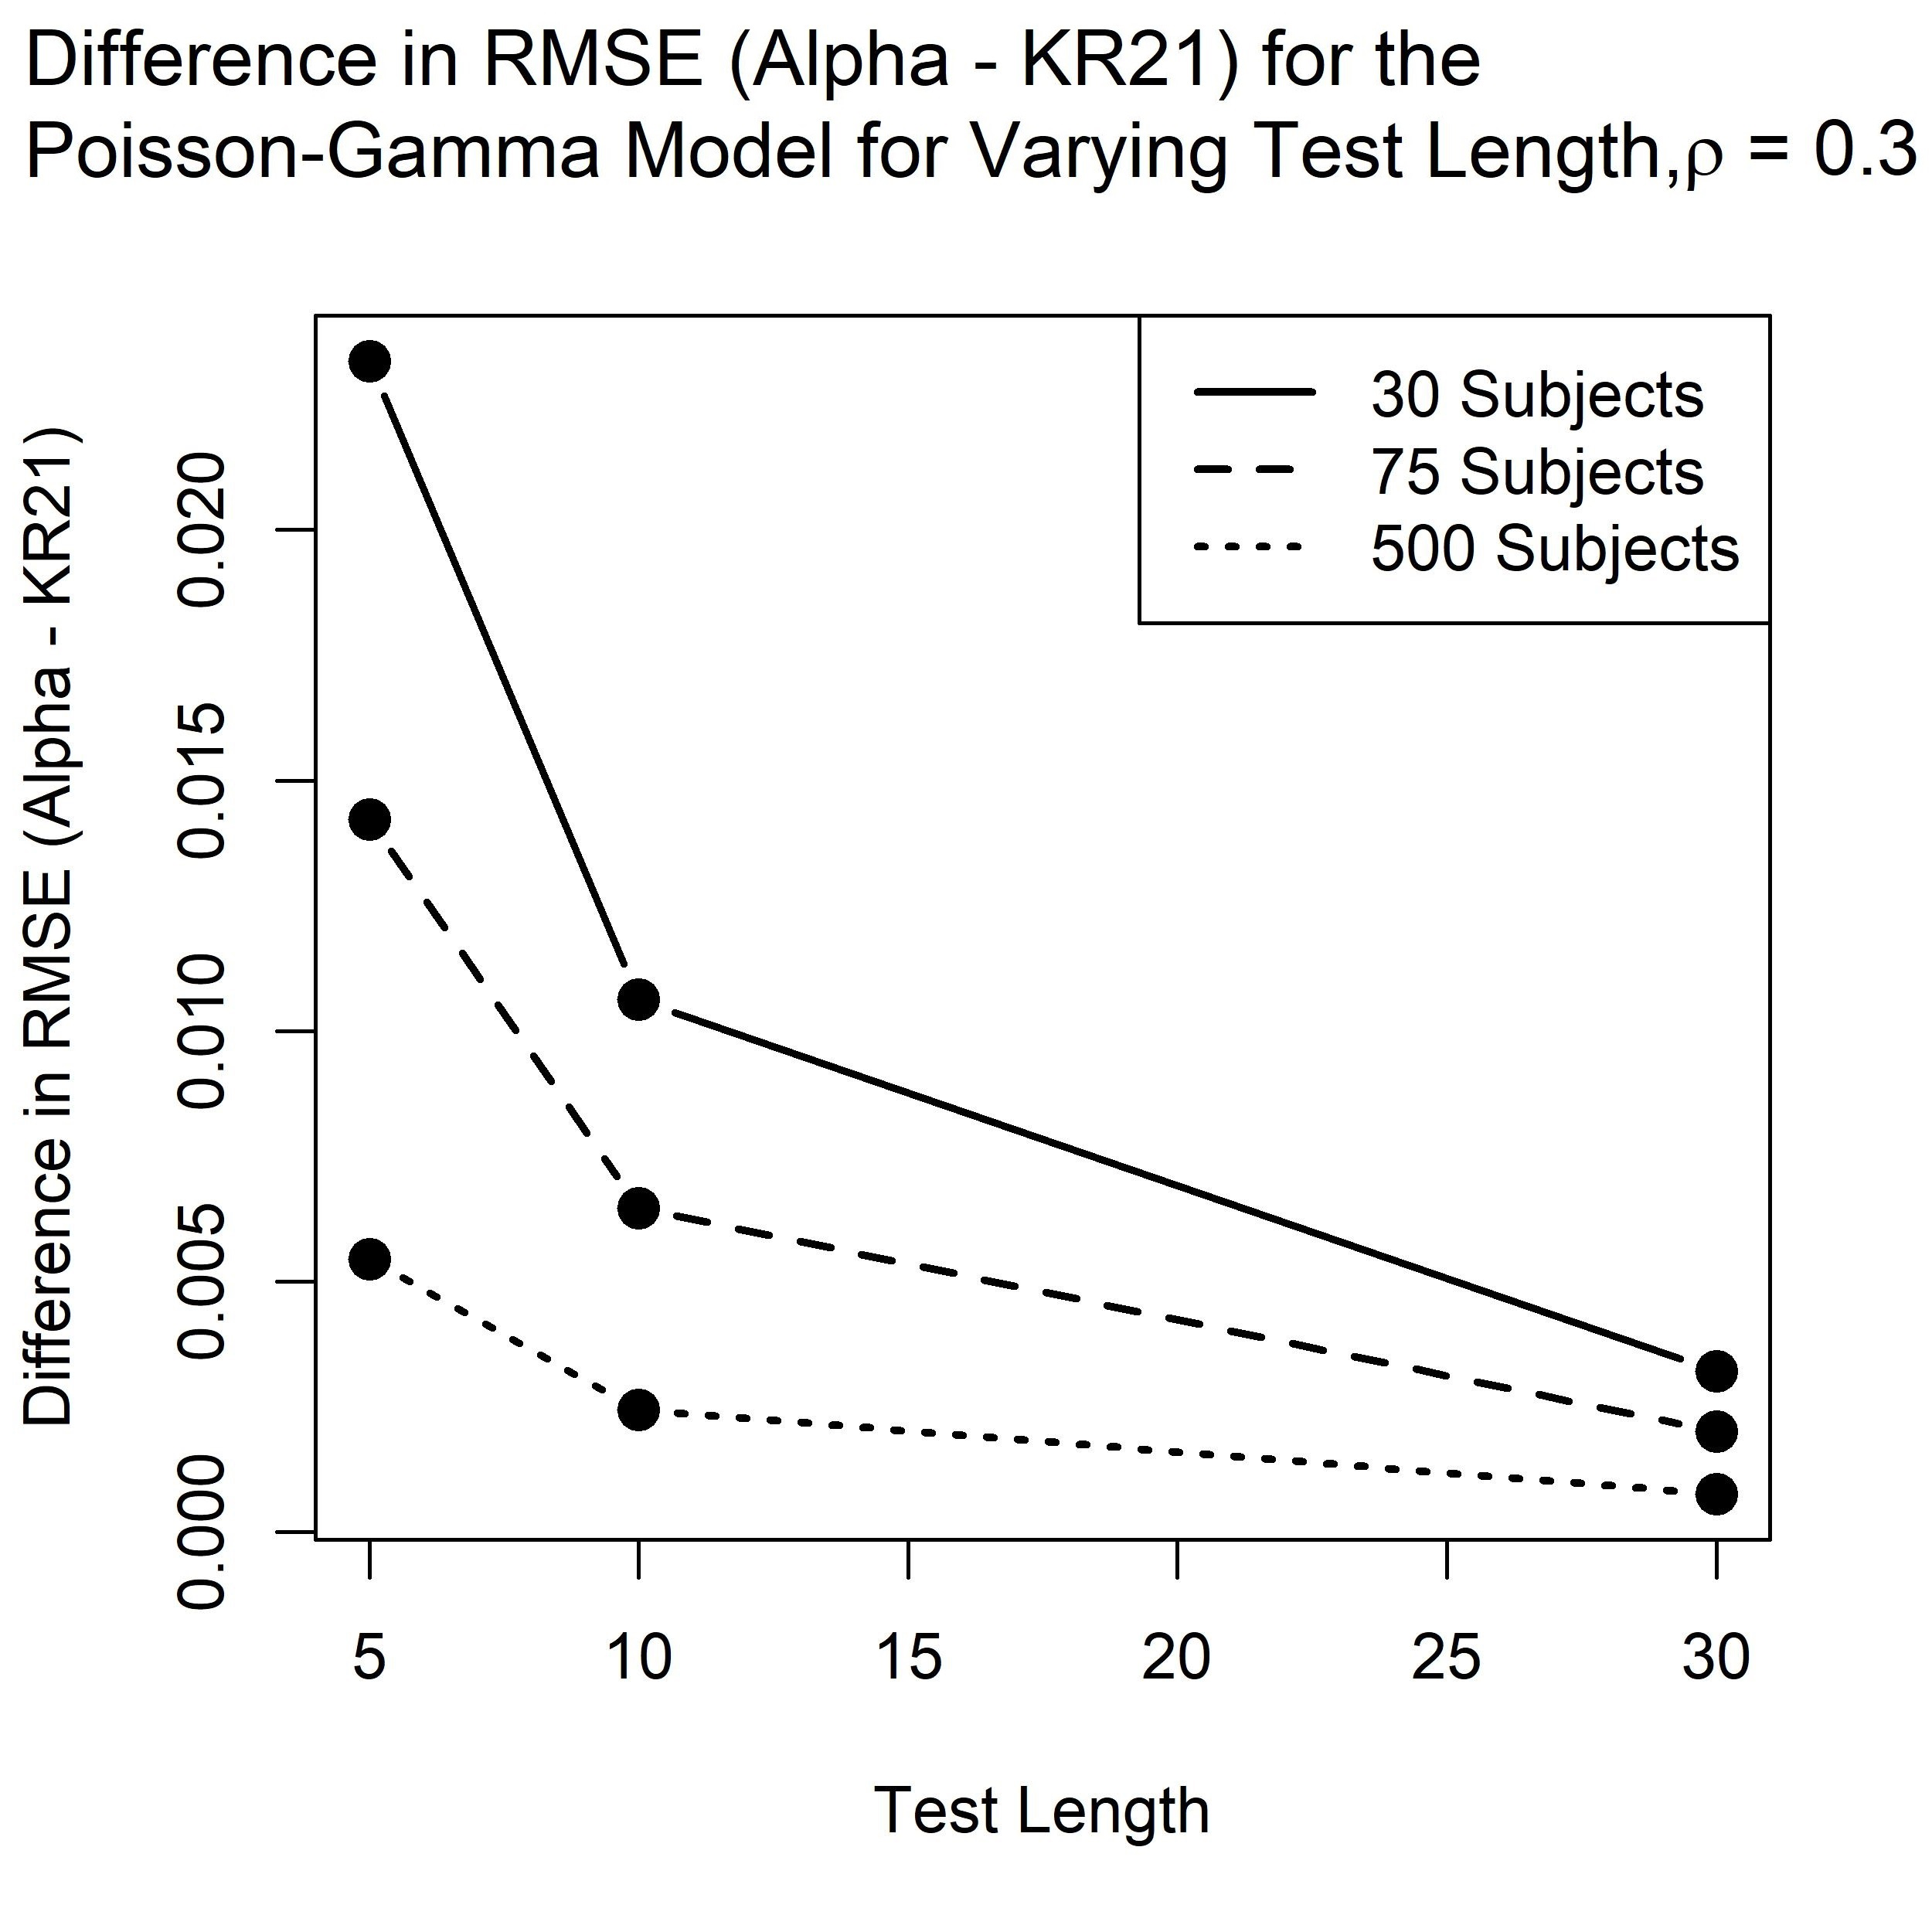
\includegraphics{PGPlot}
\caption{\color{black} Difference in RMSE (Alpha - KR21) for tests of different lengths for the poisson-gamma model with $\rho = 0.3$, grouped by number of subjects. The plot clearly shows that $\hat{\alpha}$ has a larger RMSE than KR21, but this effect decreases towards zero as both the test length $\testlength$ and number of subjects $\numsubjects$ increases. The data in this plot are from Table \ref{Tab:PoissonSimulationStudy}.}
\label{Fig:PGPlot}
\end{figure}

\begin{figure}[ht] \centering
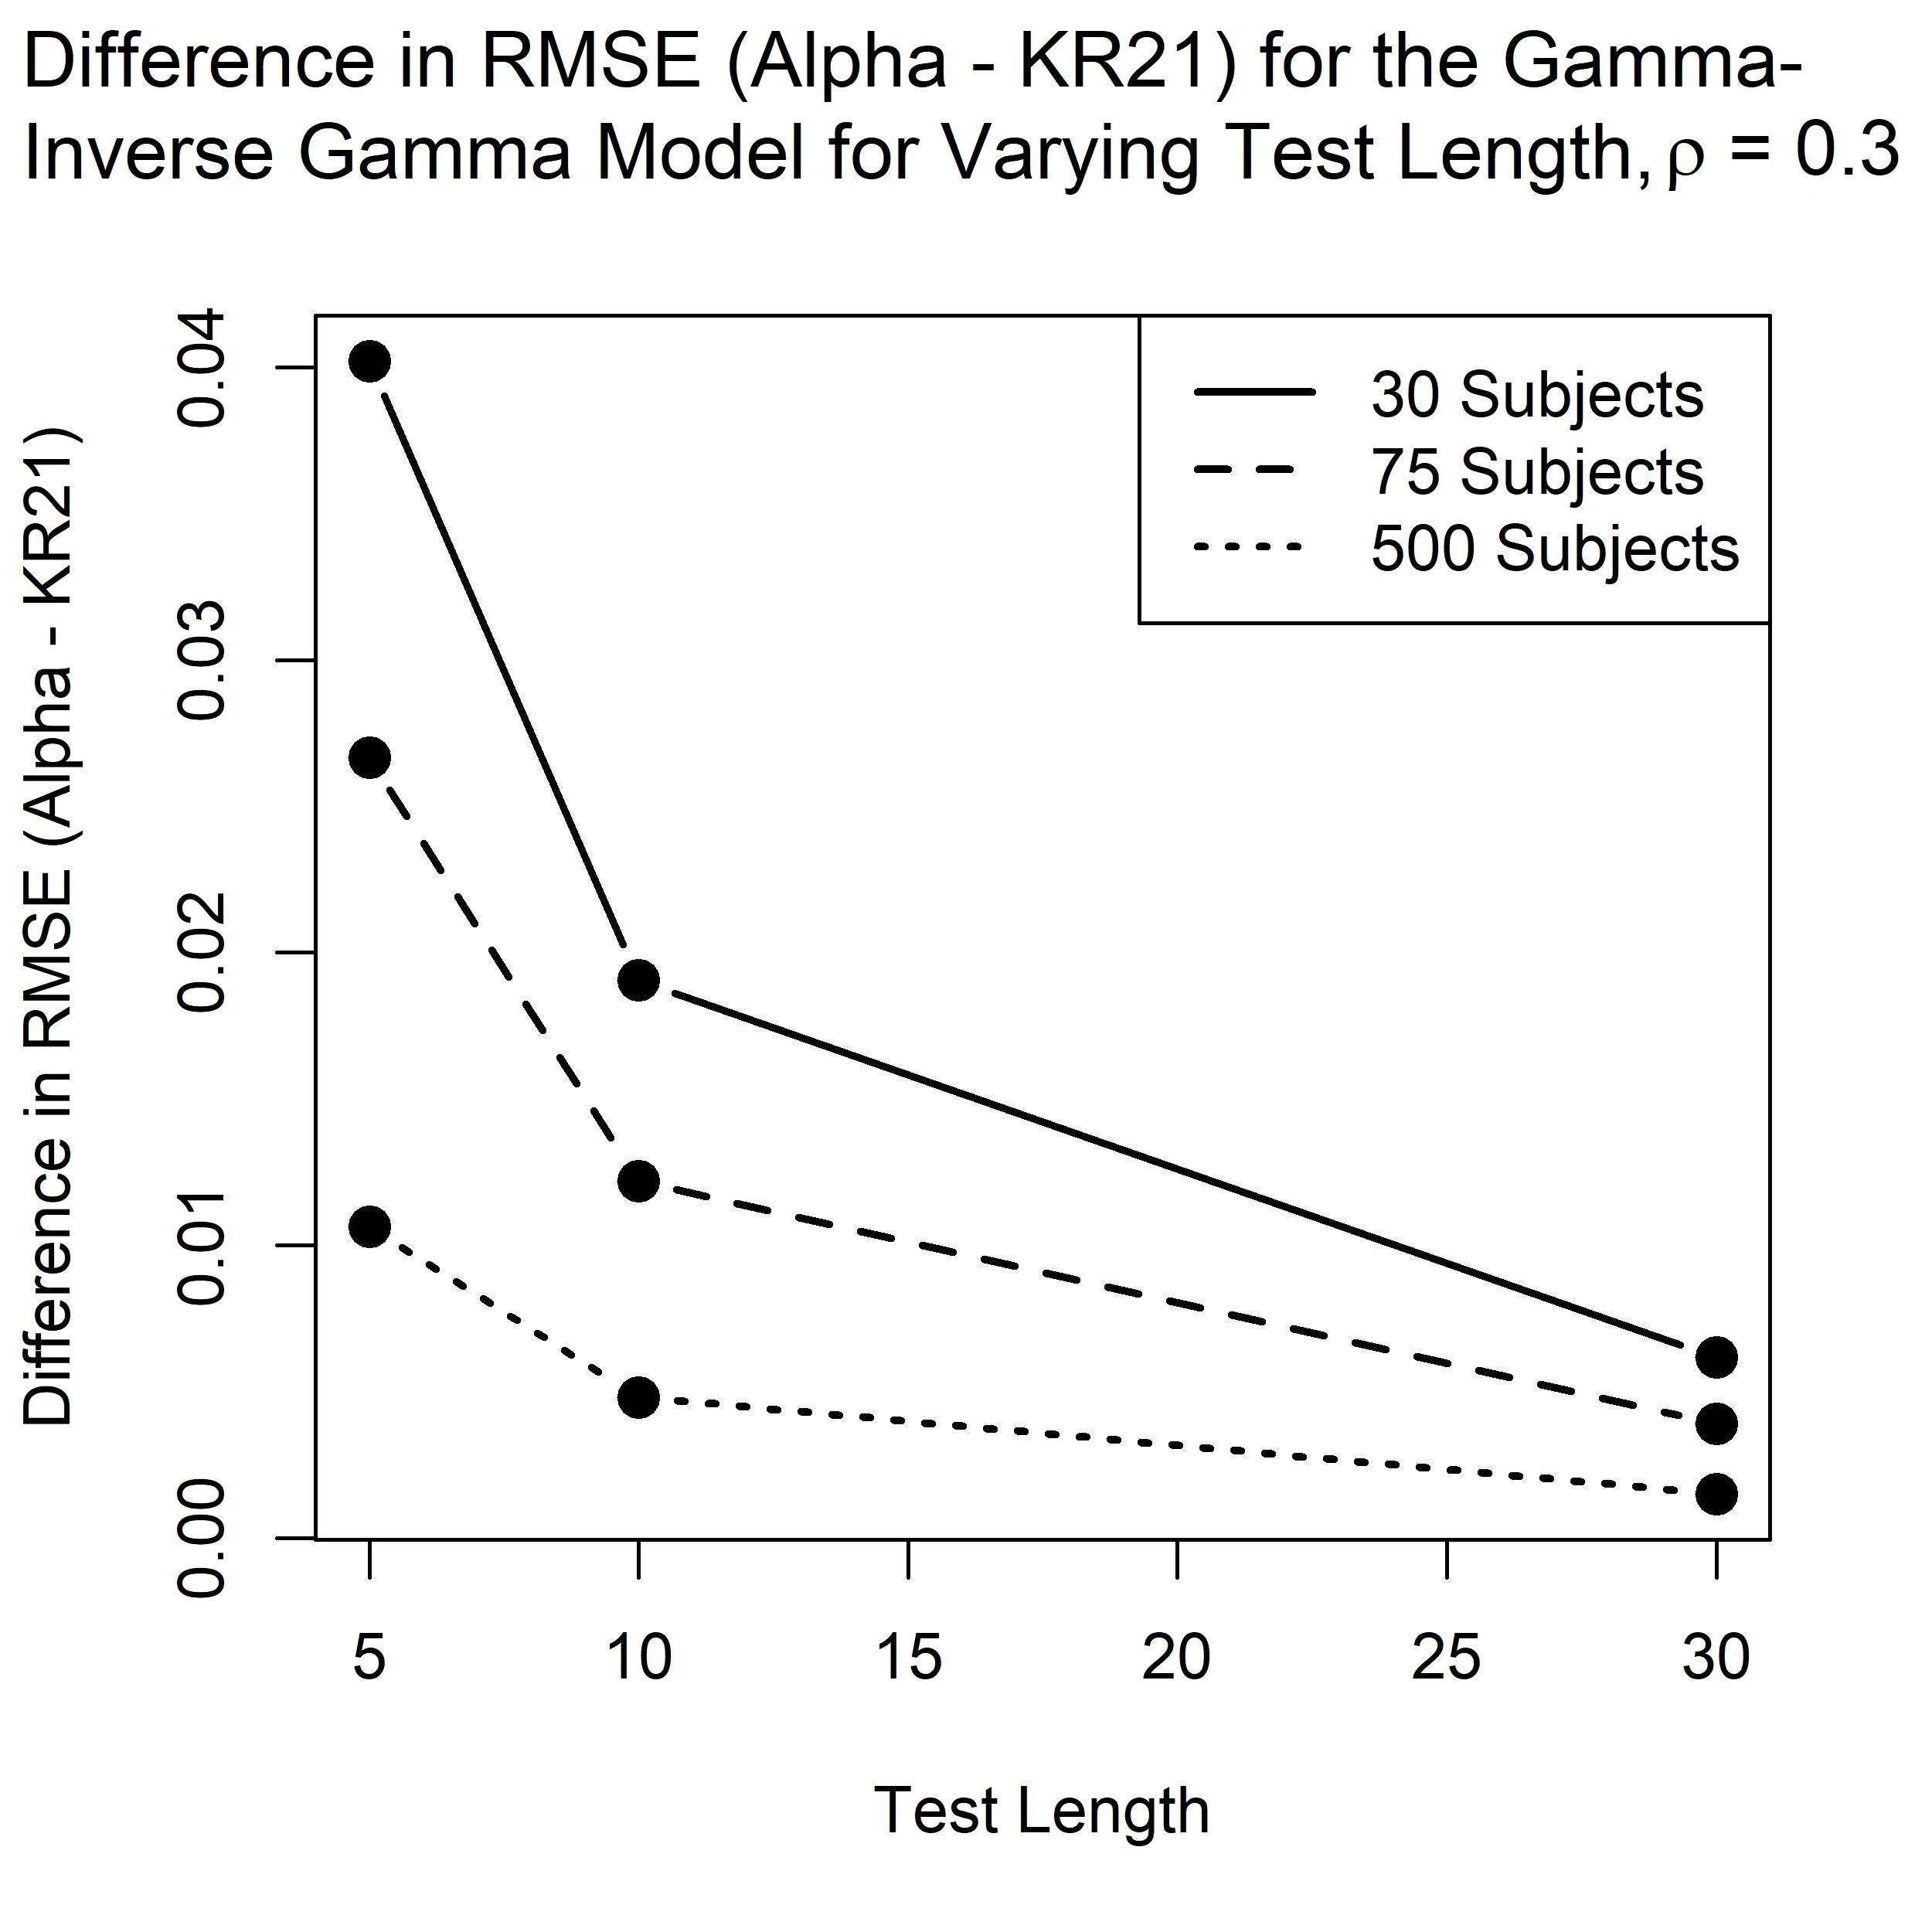
\includegraphics{GGPlot}
\caption{\color{black} Difference in RMSE (Alpha - KR21) for tests of different lengths for the gamma-inverse gamma model with $\rho = 0.3$, grouped by number of subjects. The plot clearly shows that $\hat{\alpha}$ has a larger RMSE than KR21, but this effect decreases towards zero as both the test length $\testlength$ and number of subjects $\numsubjects$ increases. The data in this plot are from Table \ref{Tab:GammaInvgammaSimulationStudy}.}
\label{Fig:GGPlot}
\end{figure}

\begin{figure}[ht] \centering
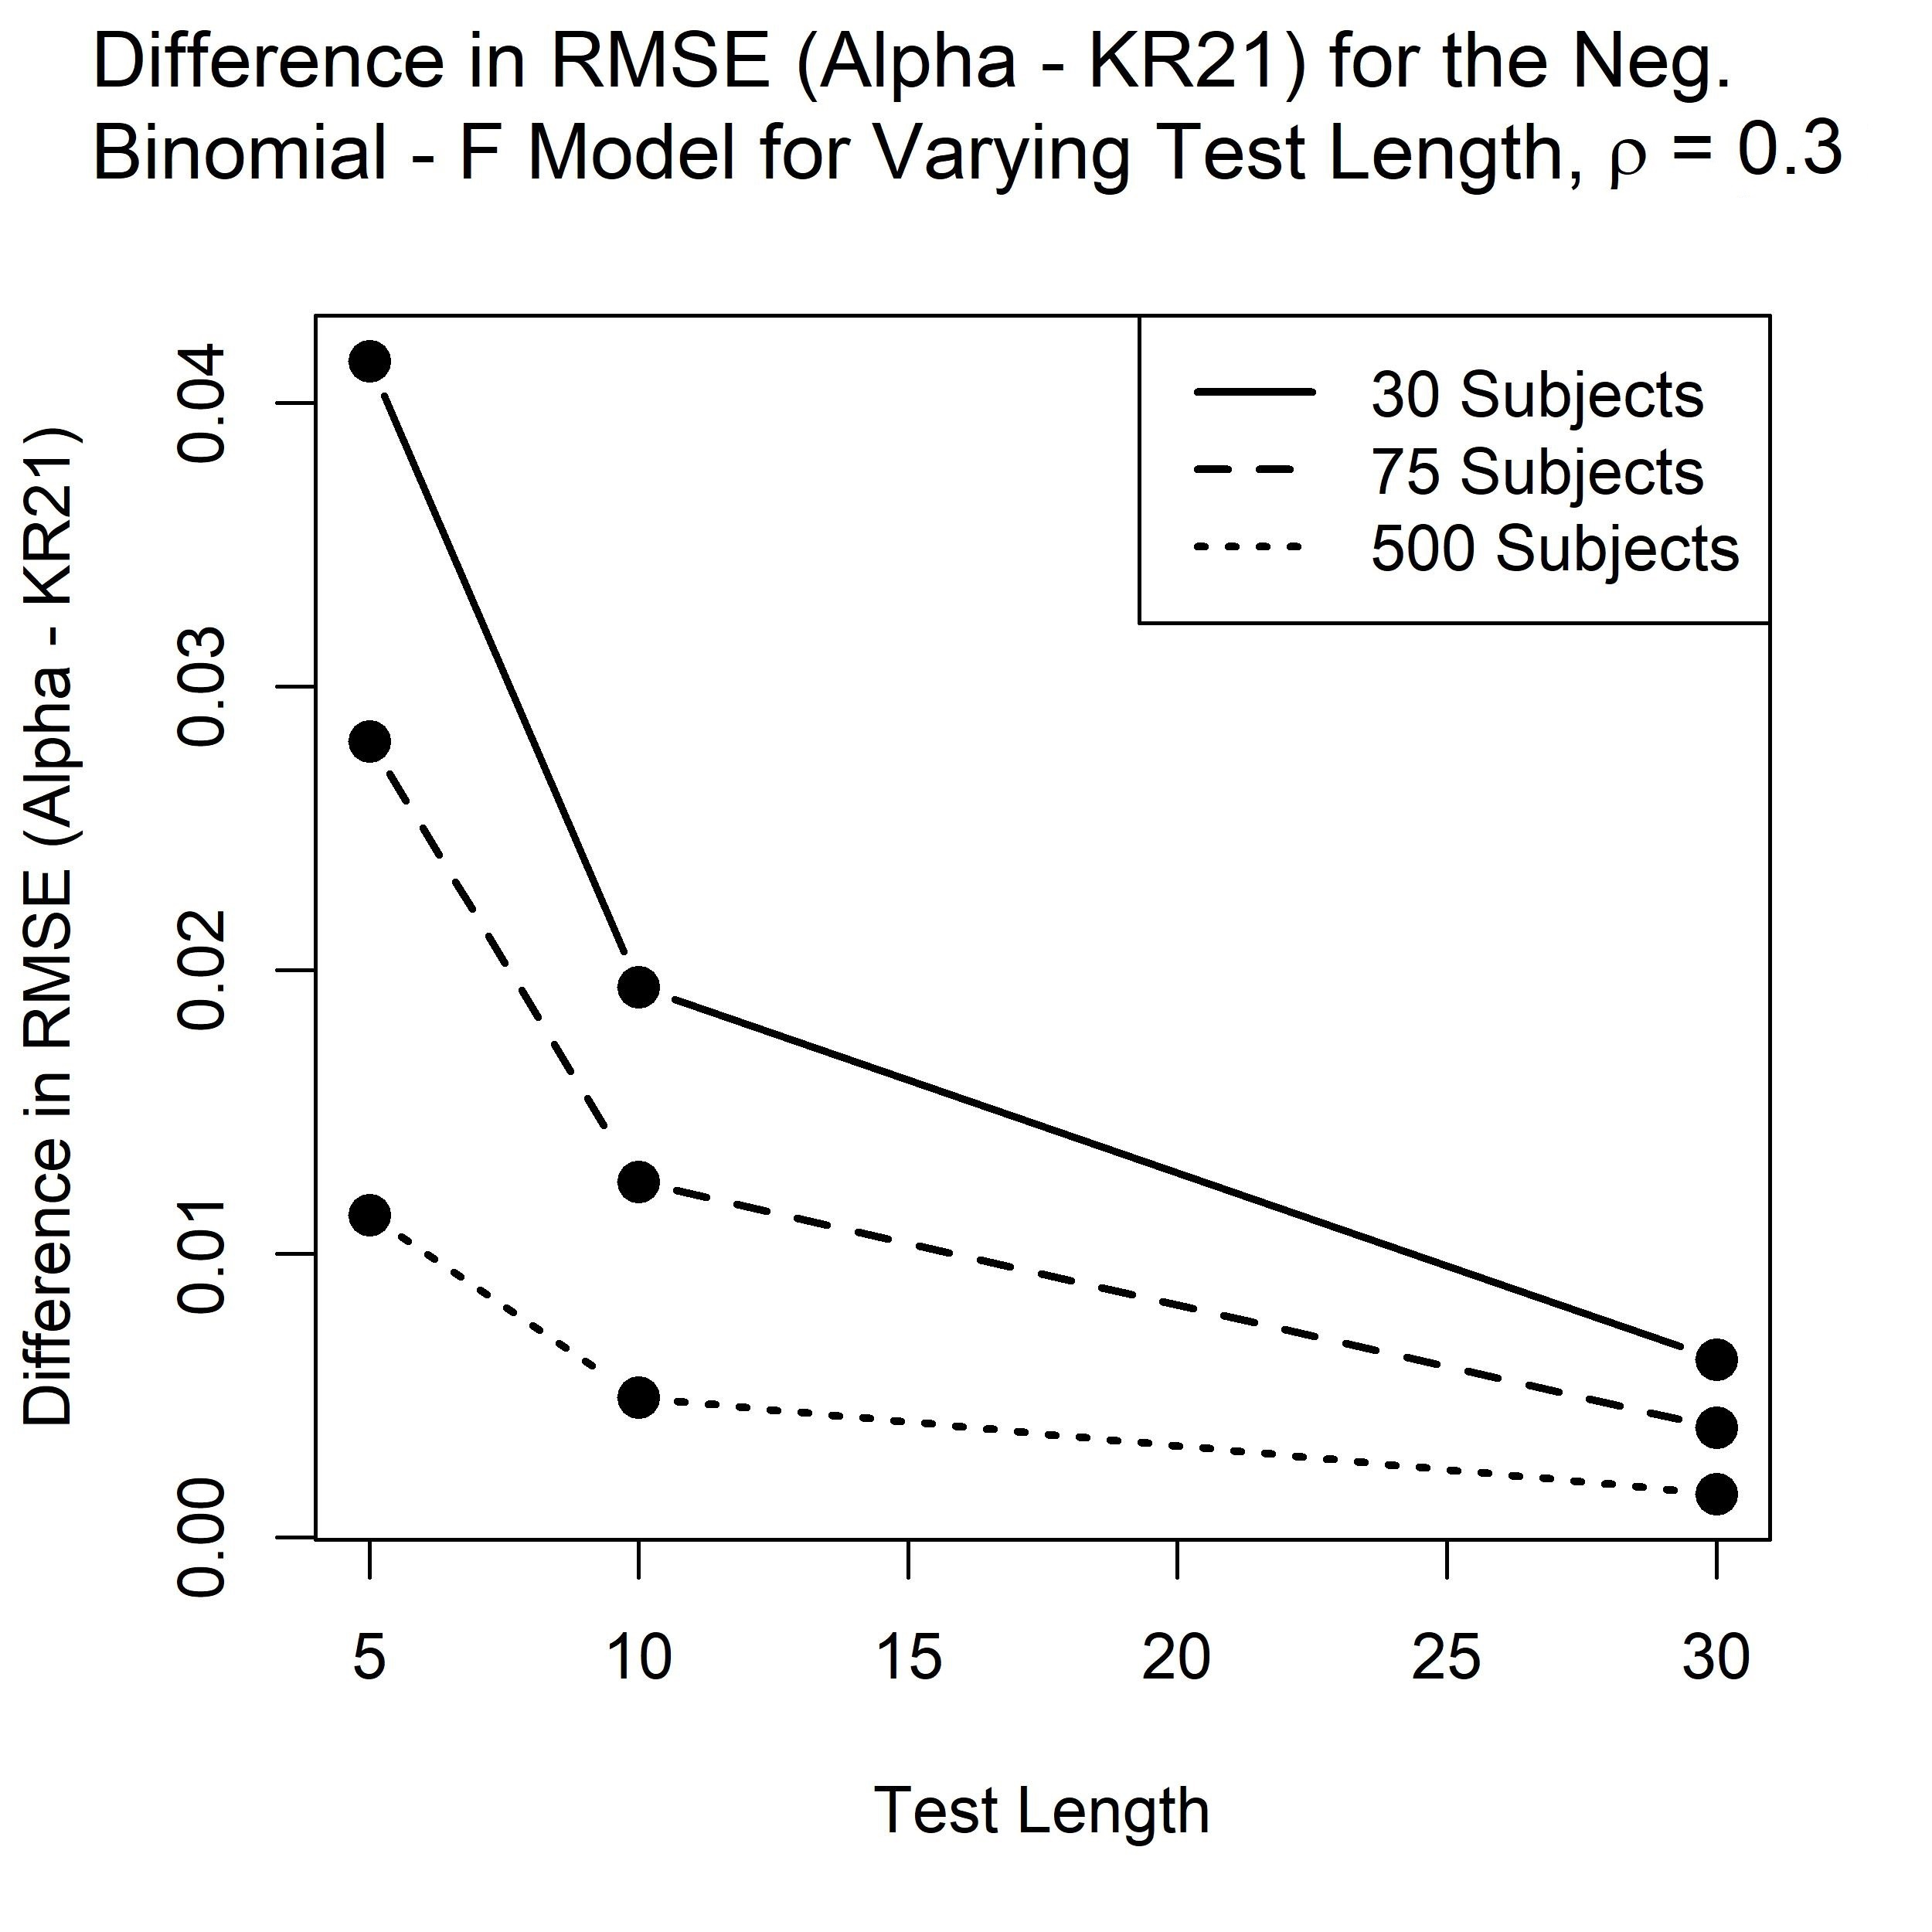
\includegraphics{NBFPlot}
\caption{\color{black} Difference in RMSE (Alpha - KR21) for tests of different lengths for the negative binomial-F model with $\rho = 0.3$, grouped by number of subjects. The plot clearly shows that $\hat{\alpha}$ has a larger RMSE than KR21, but this effect decreases towards zero as both the test length $\testlength$ and number of subjects $\numsubjects$ increases. The data in this plot are from Table \ref{Tab:NegativeBinomialFSimulationStudy}.}
\label{Fig:NBFPlot}
\end{figure}

\begin{figure}[ht] \centering
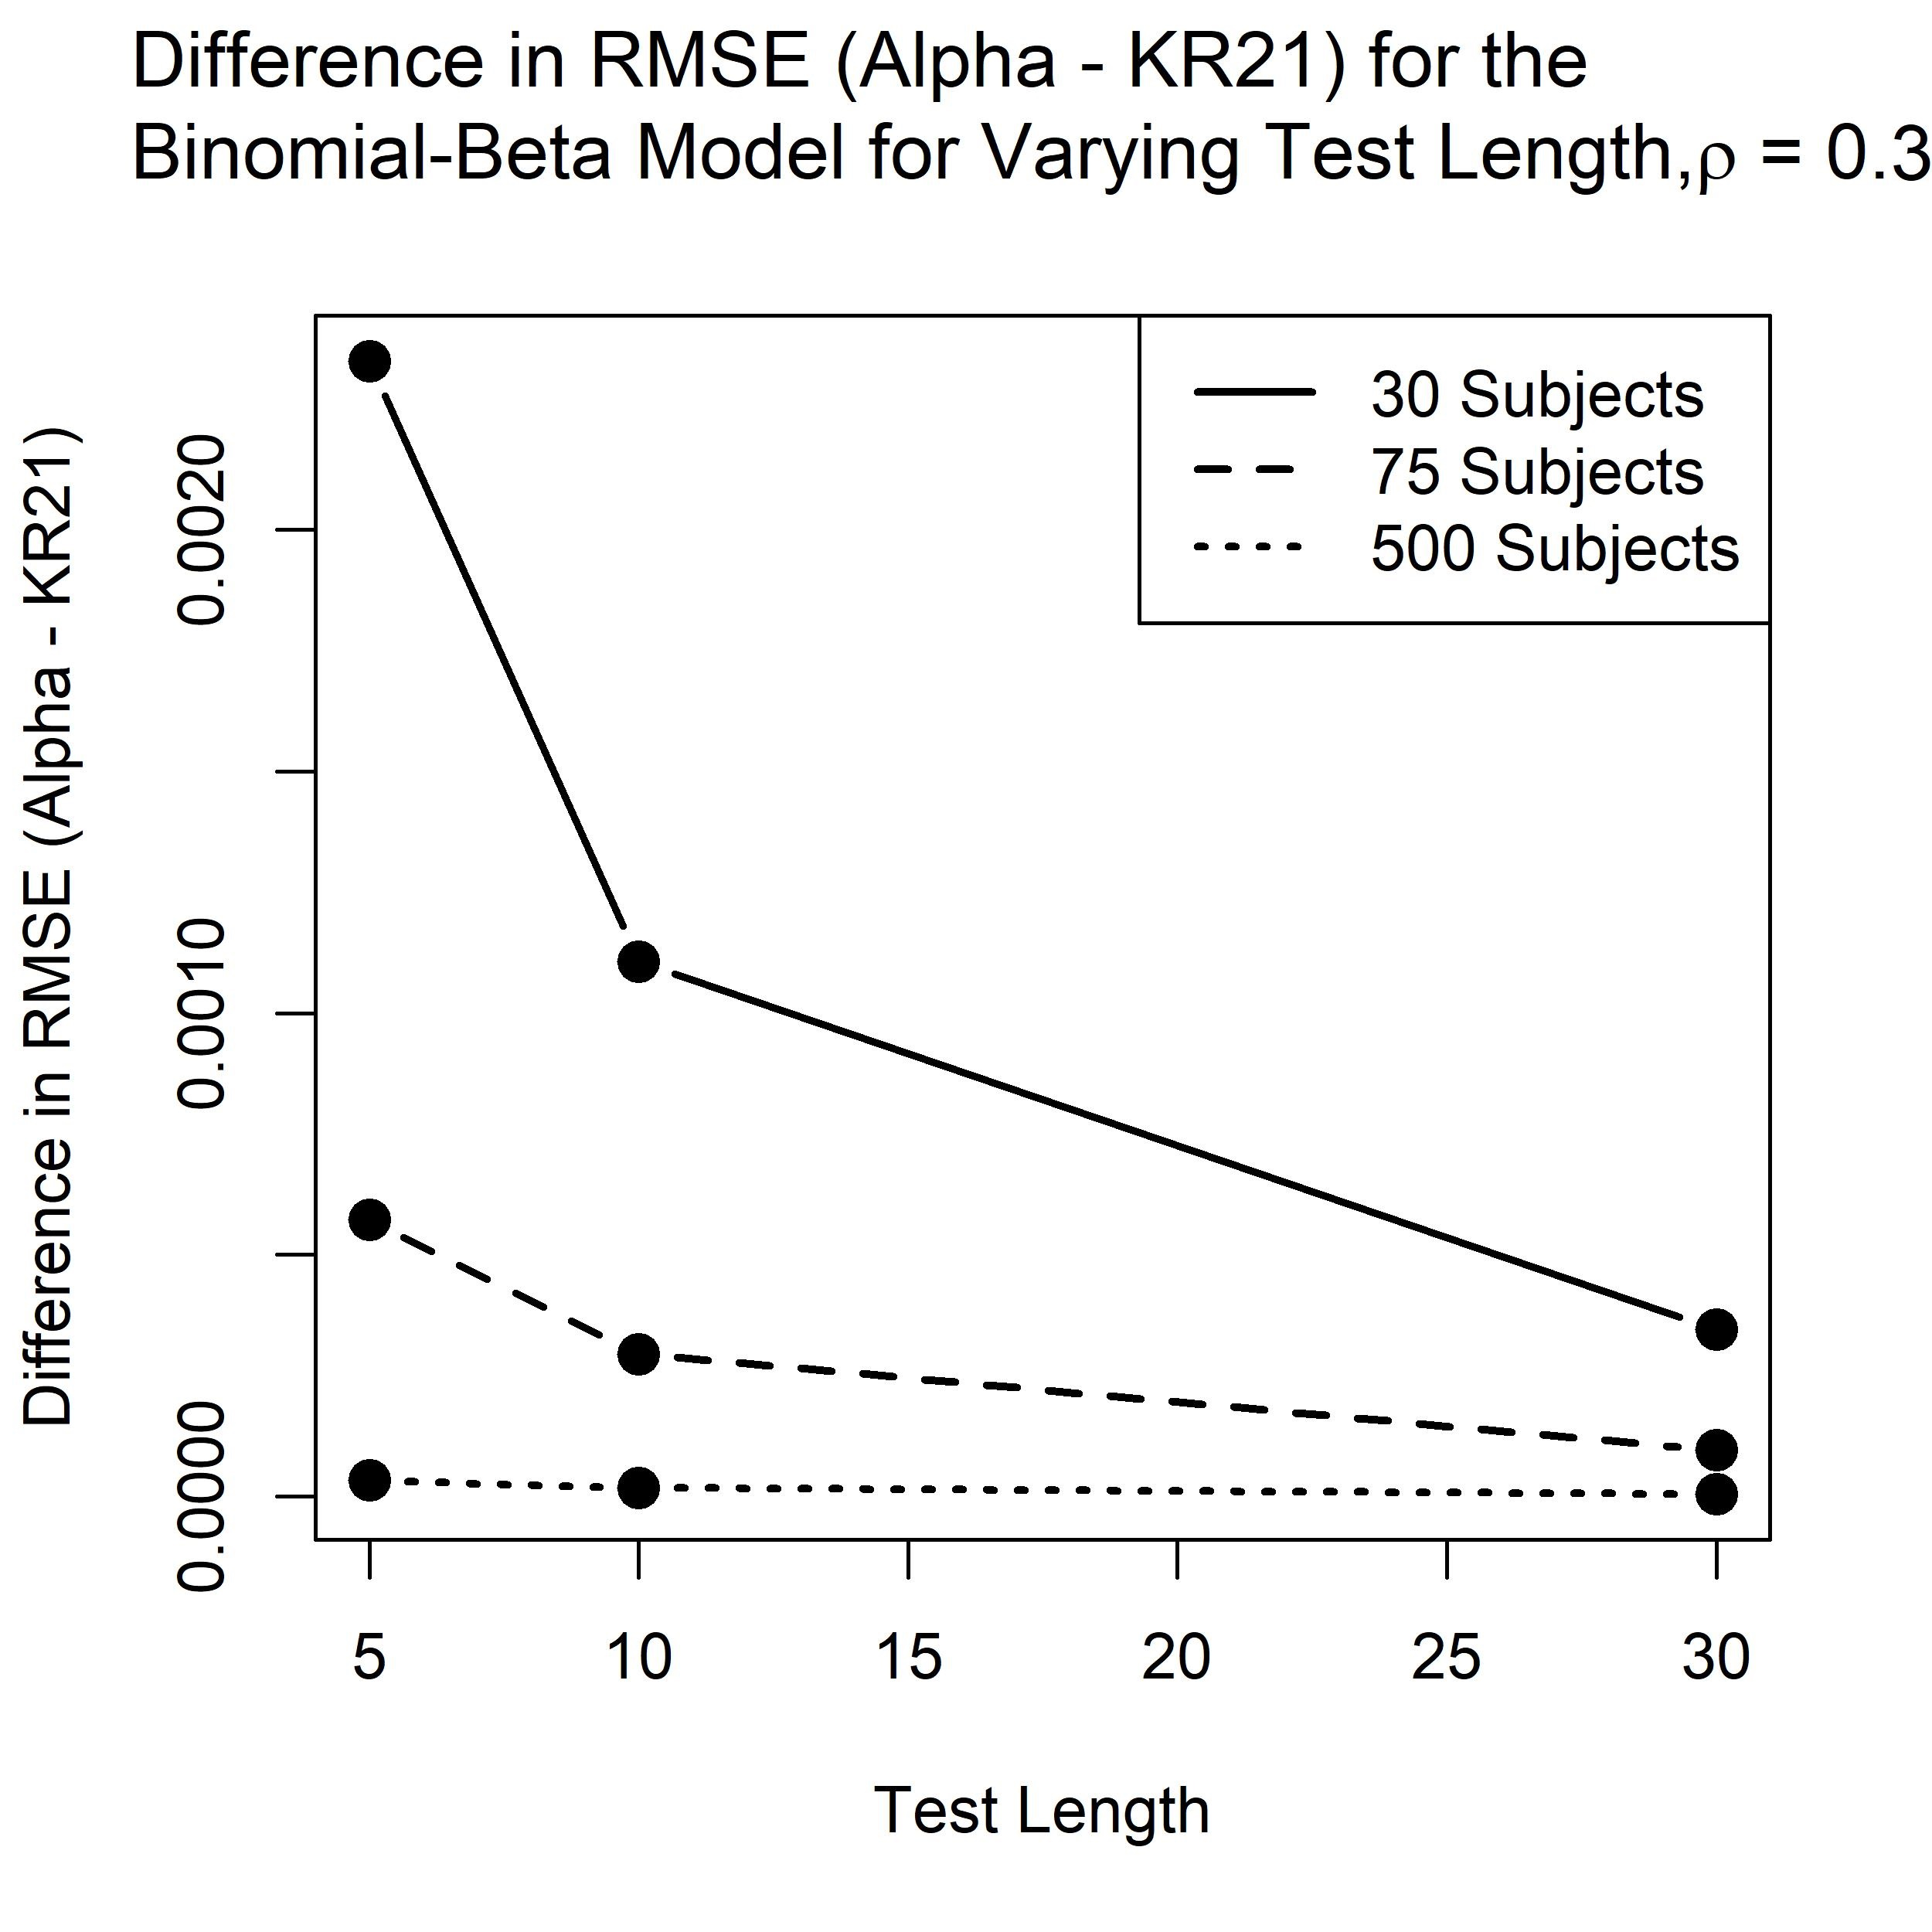
\includegraphics{BBPlot}
\caption{\color{black} Difference in RMSE (Alpha - KR21) for tests of different lengths for the binomial-beta model with $\rho = 0.3$, grouped by number of subjects. The plot clearly shows that $\hat{\alpha}$ has a larger RMSE than KR21, but this effect decreases towards zero as both the test length $\testlength$ and number of subjects $\numsubjects$ increases. The data in this plot are from Table \ref{Tab:BetaBinomialSimulationStudy}.}
\label{Fig:BBPlot}
\end{figure}



% BIBLIOGRAPHY 

\clearpage
\bibliographystyle{apacite}
%\bibliography{bibliography}
%\nocite{*}

\begin{thebibliography}{}

\bibitem [\protect \citeauthoryear {%
Allison%
}{%
Allison%
}{%
{\protect \APACyear {1978}}%
}]{%
Allison1978}
\APACinsertmetastar {%
Allison1978}%
\begin{APACrefauthors}%
Allison, P\BPBI D.%
\end{APACrefauthors}%
\unskip\
\newblock
\APACrefYearMonthDay{1978}{}{}.
\newblock
{\BBOQ}\APACrefatitle {The reliability of variables measured as the number of
  events in an interval of time} {The reliability of variables measured as the
  number of events in an interval of time}.{\BBCQ}
\newblock
\APACjournalVolNumPages{Sociological Methodology}{9}{}{238 --253}.
\PrintBackRefs{\CurrentBib}

\bibitem [\protect \citeauthoryear {%
Bay%
}{%
Bay%
}{%
{\protect \APACyear {1973}}%
}]{%
Bay1973}
\APACinsertmetastar {%
Bay1973}%
\begin{APACrefauthors}%
Bay, K\BPBI S.%
\end{APACrefauthors}%
\unskip\
\newblock
\APACrefYearMonthDay{1973}{}{}.
\newblock
{\BBOQ}\APACrefatitle {The effect of non-normality on the sampling distribution
  of standard error of reliability coefficient estimates under an analysis of
  variance model} {The effect of non-normality on the sampling distribution of
  standard error of reliability coefficient estimates under an analysis of
  variance model}.{\BBCQ}
\newblock
\APACjournalVolNumPages{British Journal of Mathematical and Statistical
  Psychology}{26}{1}{45-57}.
\PrintBackRefs{\CurrentBib}

\bibitem [\protect \citeauthoryear {%
Casella%
\ \BBA {} Berger%
}{%
Casella%
\ \BBA {} Berger%
}{%
{\protect \APACyear {2002}}%
}]{%
CasellaBerger}
\APACinsertmetastar {%
CasellaBerger}%
\begin{APACrefauthors}%
Casella, G.%
\BCBT {}\ \BBA {} Berger, R.%
\end{APACrefauthors}%
\unskip\
\newblock
\APACrefYear{2002}.
\newblock
\APACrefbtitle {Statistical Inference, Second Edition} {Statistical inference,
  second edition}.
\newblock
\APACaddressPublisher{}{Duxbury Press}.
\PrintBackRefs{\CurrentBib}

\bibitem [\protect \citeauthoryear {%
Cronbach%
}{%
Cronbach%
}{%
{\protect \APACyear {1951}}%
}]{%
Cronbach1951}
\APACinsertmetastar {%
Cronbach1951}%
\begin{APACrefauthors}%
Cronbach, L\BPBI J.%
\end{APACrefauthors}%
\unskip\
\newblock
\APACrefYearMonthDay{1951}{September}{}.
\newblock
{\BBOQ}\APACrefatitle {Coefficient alpha and the internal structure of tests}
  {Coefficient alpha and the internal structure of tests}.{\BBCQ}
\newblock
\APACjournalVolNumPages{Psychometrika}{16}{3}{297 -- 334}.
\PrintBackRefs{\CurrentBib}

\bibitem [\protect \citeauthoryear {%
L\BPBI J.~Feldt%
}{%
L\BPBI J.~Feldt%
}{%
{\protect \APACyear {1984}}%
}]{%
Feldt1984}
\APACinsertmetastar {%
Feldt1984}%
\begin{APACrefauthors}%
Feldt, L\BPBI J.%
\end{APACrefauthors}%
\unskip\
\newblock
\APACrefYearMonthDay{1984}{}{}.
\newblock
{\BBOQ}\APACrefatitle {Some relationships between the binomial error model and
  classical test theory} {Some relationships between the binomial error model
  and classical test theory}.{\BBCQ}
\newblock
\APACjournalVolNumPages{Educational and Psychological Measurement}{44}{4}{883
  -- 891}.
\PrintBackRefs{\CurrentBib}

\bibitem [\protect \citeauthoryear {%
L\BPBI S.~Feldt%
}{%
L\BPBI S.~Feldt%
}{%
{\protect \APACyear {1965}}%
}]{%
Feldt1965}
\APACinsertmetastar {%
Feldt1965}%
\begin{APACrefauthors}%
Feldt, L\BPBI S.%
\end{APACrefauthors}%
\unskip\
\newblock
\APACrefYearMonthDay{1965}{September}{}.
\newblock
{\BBOQ}\APACrefatitle {The approximate sampling distribution of
  Kuder-Richardson reliability coefficient twenty} {The approximate sampling
  distribution of kuder-richardson reliability coefficient twenty}.{\BBCQ}
\newblock
\APACjournalVolNumPages{Psychometrika}{30}{3}{357 -- 370}.
\PrintBackRefs{\CurrentBib}

\bibitem [\protect \citeauthoryear {%
Foster%
}{%
Foster%
}{%
{\protect \APACyear {2020}}%
}]{%
Foster2020}
\APACinsertmetastar {%
Foster2020}%
\begin{APACrefauthors}%
Foster, R\BPBI C.%
\end{APACrefauthors}%
\unskip\
\newblock
\APACrefYearMonthDay{2020}{{\APACmonth{06}}}{}.
\newblock
{\BBOQ}\APACrefatitle {A Generalized Framework for Classical Test Theory} {A
  generalized framework for classical test theory}.{\BBCQ}
\newblock
\APACjournalVolNumPages{The Journal of Mathematical Psychology}{96}{}{}.
\PrintBackRefs{\CurrentBib}

\bibitem [\protect \citeauthoryear {%
Geldhof%
, Preacher%
\BCBL {}\ \BBA {} Zyphur%
}{%
Geldhof%
\ \protect \BOthers {.}}{%
{\protect \APACyear {2014}}%
}]{%
Geldhof2014}
\APACinsertmetastar {%
Geldhof2014}%
\begin{APACrefauthors}%
Geldhof, G\BPBI J.%
, Preacher, K\BPBI J.%
\BCBL {}\ \BBA {} Zyphur, M\BPBI J.%
\end{APACrefauthors}%
\unskip\
\newblock
\APACrefYearMonthDay{2014}{}{}.
\newblock
{\BBOQ}\APACrefatitle {Reliability Estimation in a Multilevel Confirmatory
  Factor Analysis Framework} {Reliability estimation in a multilevel
  confirmatory factor analysis framework}.{\BBCQ}
\newblock
\APACjournalVolNumPages{Psychological Methods}{19}{1}{72-91}.
\PrintBackRefs{\CurrentBib}

\bibitem [\protect \citeauthoryear {%
Hayes%
\ \BBA {} Coutts%
}{%
Hayes%
\ \BBA {} Coutts%
}{%
{\protect \APACyear {2020}}%
}]{%
Hayes2020}
\APACinsertmetastar {%
Hayes2020}%
\begin{APACrefauthors}%
Hayes, A\BPBI F.%
\BCBT {}\ \BBA {} Coutts, J\BPBI J.%
\end{APACrefauthors}%
\unskip\
\newblock
\APACrefYearMonthDay{2020}{}{}.
\newblock
{\BBOQ}\APACrefatitle {Use Omega Rather than Cronbach’s Alpha for Estimating
  Reliability. But…} {Use omega rather than cronbach’s alpha for estimating
  reliability. but…}.{\BBCQ}
\newblock
\APACjournalVolNumPages{Communication Methods and Measures}{14}{1}{1-24}.
\PrintBackRefs{\CurrentBib}

\bibitem [\protect \citeauthoryear {%
Huynh%
}{%
Huynh%
}{%
{\protect \APACyear {1979}}%
}]{%
Huynh1979}
\APACinsertmetastar {%
Huynh1979}%
\begin{APACrefauthors}%
Huynh, H.%
\end{APACrefauthors}%
\unskip\
\newblock
\APACrefYearMonthDay{1979}{}{}.
\newblock
{\BBOQ}\APACrefatitle {Statistical Inference for two Reliability Indices in
  Mastery Testing Based on the Beta-Binomial Model} {Statistical inference for
  two reliability indices in mastery testing based on the beta-binomial
  model}.{\BBCQ}
\newblock
\APACjournalVolNumPages{Journal of Educational Statistics}{4}{3}{231-246}.
\PrintBackRefs{\CurrentBib}

\bibitem [\protect \citeauthoryear {%
Keats%
\ \BBA {} Lord%
}{%
Keats%
\ \BBA {} Lord%
}{%
{\protect \APACyear {1962}}%
}]{%
Keats1962}
\APACinsertmetastar {%
Keats1962}%
\begin{APACrefauthors}%
Keats, J\BPBI A.%
\BCBT {}\ \BBA {} Lord, F\BPBI M.%
\end{APACrefauthors}%
\unskip\
\newblock
\APACrefYearMonthDay{1962}{March}{}.
\newblock
{\BBOQ}\APACrefatitle {A theoretical distribution for mental test scores} {A
  theoretical distribution for mental test scores}.{\BBCQ}
\newblock
\APACjournalVolNumPages{Psychometrika}{27}{1}{59 -- 72}.
\PrintBackRefs{\CurrentBib}

\bibitem [\protect \citeauthoryear {%
Kuder%
\ \BBA {} Richardson%
}{%
Kuder%
\ \BBA {} Richardson%
}{%
{\protect \APACyear {1937}}%
}]{%
Kuder1937}
\APACinsertmetastar {%
Kuder1937}%
\begin{APACrefauthors}%
Kuder, G\BPBI F.%
\BCBT {}\ \BBA {} Richardson, M\BPBI W.%
\end{APACrefauthors}%
\unskip\
\newblock
\APACrefYearMonthDay{1937}{}{}.
\newblock
{\BBOQ}\APACrefatitle {The theory of the estimation of test reliability} {The
  theory of the estimation of test reliability}.{\BBCQ}
\newblock
\APACjournalVolNumPages{Psychometrika}{2}{3}{151 -- 160}.
\PrintBackRefs{\CurrentBib}

\bibitem [\protect \citeauthoryear {%
Lord%
}{%
Lord%
}{%
{\protect \APACyear {1965}}%
}]{%
Lord1965}
\APACinsertmetastar {%
Lord1965}%
\begin{APACrefauthors}%
Lord, F\BPBI M.%
\end{APACrefauthors}%
\unskip\
\newblock
\APACrefYearMonthDay{1965}{September}{}.
\newblock
{\BBOQ}\APACrefatitle {A strong true-score theory, with applications} {A strong
  true-score theory, with applications}.{\BBCQ}
\newblock
\APACjournalVolNumPages{Psychometrika}{30}{3}{239 -- 270}.
\PrintBackRefs{\CurrentBib}

\bibitem [\protect \citeauthoryear {%
Lord%
, Novick%
\BCBL {}\ \BBA {} Birnbaum%
}{%
Lord%
\ \protect \BOthers {.}}{%
{\protect \APACyear {1968}}%
}]{%
Lord1968}
\APACinsertmetastar {%
Lord1968}%
\begin{APACrefauthors}%
Lord, F\BPBI M.%
, Novick, M\BPBI R.%
\BCBL {}\ \BBA {} Birnbaum, A.%
\end{APACrefauthors}%
\unskip\
\newblock
\APACrefYear{1968}.
\newblock
\APACrefbtitle {Statistical theories of mental test scores} {Statistical
  theories of mental test scores}.
\newblock
\APACaddressPublisher{Oxford, England}{Addison-Wesley}.
\PrintBackRefs{\CurrentBib}

\bibitem [\protect \citeauthoryear {%
McDonald%
}{%
McDonald%
}{%
{\protect \APACyear {1999}}%
}]{%
Mcdonald1999}
\APACinsertmetastar {%
Mcdonald1999}%
\begin{APACrefauthors}%
McDonald, R.%
\end{APACrefauthors}%
\unskip\
\newblock
\APACrefYear{1999}.
\newblock
\APACrefbtitle {Test Theory: A Unified Treatment} {Test theory: A unified
  treatment}.
\newblock
\APACaddressPublisher{}{Taylor \& Francis}.
\PrintBackRefs{\CurrentBib}

\bibitem [\protect \citeauthoryear {%
McNeish%
}{%
McNeish%
}{%
{\protect \APACyear {2018}}%
}]{%
Mcneish2017}
\APACinsertmetastar {%
Mcneish2017}%
\begin{APACrefauthors}%
McNeish, D.%
\end{APACrefauthors}%
\unskip\
\newblock
\APACrefYearMonthDay{2018}{}{}.
\newblock
{\BBOQ}\APACrefatitle {Thanks coefficient alpha, we'll take it from here}
  {Thanks coefficient alpha, we'll take it from here}.{\BBCQ}
\newblock
\APACjournalVolNumPages{Psychological Methods}{23}{3}{412-433}.
\PrintBackRefs{\CurrentBib}

\bibitem [\protect \citeauthoryear {%
Meredith%
}{%
Meredith%
}{%
{\protect \APACyear {1971}}%
}]{%
Meredith1971}
\APACinsertmetastar {%
Meredith1971}%
\begin{APACrefauthors}%
Meredith, W.%
\end{APACrefauthors}%
\unskip\
\newblock
\APACrefYearMonthDay{1971}{08}{}.
\newblock
{\BBOQ}\APACrefatitle {Poisson distributions of error in mental test theory}
  {Poisson distributions of error in mental test theory}.{\BBCQ}
\newblock
\APACjournalVolNumPages{British Journal of Mathematical and Statistical
  Psychology}{24}{}{49 - 82}.
\PrintBackRefs{\CurrentBib}

\bibitem [\protect \citeauthoryear {%
Moore%
}{%
Moore%
}{%
{\protect \APACyear {1970}}%
}]{%
Moore1970}
\APACinsertmetastar {%
Moore1970}%
\begin{APACrefauthors}%
Moore, W\BPBI E.%
\end{APACrefauthors}%
\unskip\
\newblock
\APACrefYearMonthDay{1970}{November}{}.
\newblock
\APACrefbtitle {Stochastic processes as true-score models for highly speeded
  mental tests} {Stochastic processes as true-score models for highly speeded
  mental tests}\ \APACbVolEdTR{}{\BTR{}}.
\newblock
\APACaddressInstitution{Princeton, New Jersey}{Educational Testing Service}.
\PrintBackRefs{\CurrentBib}

\bibitem [\protect \citeauthoryear {%
Morris%
}{%
Morris%
}{%
{\protect \APACyear {1982}}%
}]{%
Morris1982}
\APACinsertmetastar {%
Morris1982}%
\begin{APACrefauthors}%
Morris, C\BPBI N.%
\end{APACrefauthors}%
\unskip\
\newblock
\APACrefYearMonthDay{1982}{}{}.
\newblock
{\BBOQ}\APACrefatitle {Natural exponential families with quadratic variance
  functions} {Natural exponential families with quadratic variance
  functions}.{\BBCQ}
\newblock
\APACjournalVolNumPages{The Annals of Statistics}{10}{1}{65 -- 80}.
\PrintBackRefs{\CurrentBib}

\bibitem [\protect \citeauthoryear {%
Morris%
}{%
Morris%
}{%
{\protect \APACyear {1983}}%
}]{%
Morris1983}
\APACinsertmetastar {%
Morris1983}%
\begin{APACrefauthors}%
Morris, C\BPBI N.%
\end{APACrefauthors}%
\unskip\
\newblock
\APACrefYearMonthDay{1983}{}{}.
\newblock
{\BBOQ}\APACrefatitle {Natural exponential families with quadratic variance
  functions: Statistical theory} {Natural exponential families with quadratic
  variance functions: Statistical theory}.{\BBCQ}
\newblock
\APACjournalVolNumPages{The Annals of Statistics}{11}{2}{515 -- 529}.
\PrintBackRefs{\CurrentBib}

\bibitem [\protect \citeauthoryear {%
Rasch%
}{%
Rasch%
}{%
{\protect \APACyear {1960}}%
}]{%
Rasch1960}
\APACinsertmetastar {%
Rasch1960}%
\begin{APACrefauthors}%
Rasch, G.%
\end{APACrefauthors}%
\unskip\
\newblock
\APACrefYear{1960}.
\newblock
\APACrefbtitle {Probabilistic Models for Some Intelligence and Attainment
  Tests} {Probabilistic models for some intelligence and attainment tests}.
\newblock
\APACaddressPublisher{}{Danmarks Paedagogiske Institut}.
\PrintBackRefs{\CurrentBib}

\bibitem [\protect \citeauthoryear {%
Raykov%
}{%
Raykov%
}{%
{\protect \APACyear {1998}}%
}]{%
Raykov1998}
\APACinsertmetastar {%
Raykov1998}%
\begin{APACrefauthors}%
Raykov, T.%
\end{APACrefauthors}%
\unskip\
\newblock
\APACrefYearMonthDay{1998}{}{}.
\newblock
{\BBOQ}\APACrefatitle {A Method for Obtaining Standard Errors and Confidence
  Intervals of Composite Reliability for Congeneric Items} {A method for
  obtaining standard errors and confidence intervals of composite reliability
  for congeneric items}.{\BBCQ}
\newblock
\APACjournalVolNumPages{Applied Psychological Measurement}{22}{4}{369-374}.
\PrintBackRefs{\CurrentBib}

\bibitem [\protect \citeauthoryear {%
Raykov%
\ \BBA {} Marcoulides%
}{%
Raykov%
\ \BBA {} Marcoulides%
}{%
{\protect \APACyear {2019}}%
}]{%
Raykov2019}
\APACinsertmetastar {%
Raykov2019}%
\begin{APACrefauthors}%
Raykov, T.%
\BCBT {}\ \BBA {} Marcoulides, G\BPBI A.%
\end{APACrefauthors}%
\unskip\
\newblock
\APACrefYearMonthDay{2019}{}{}.
\newblock
{\BBOQ}\APACrefatitle {Thanks Coefficient Alpha, We Still Need You!} {Thanks
  coefficient alpha, we still need you!}{\BBCQ}
\newblock
\APACjournalVolNumPages{Educational and Psychological
  Measurement}{79}{1}{200-210}.
\PrintBackRefs{\CurrentBib}

\bibitem [\protect \citeauthoryear {%
Revelle%
}{%
Revelle%
}{%
{\protect \APACyear {2020}}%
}]{%
PsychPackage}
\APACinsertmetastar {%
PsychPackage}%
\begin{APACrefauthors}%
Revelle, W.%
\end{APACrefauthors}%
\unskip\
\newblock
\APACrefYearMonthDay{2020}{}{}.
\newblock
{\BBOQ}\APACrefatitle {psych: Procedures for Psychological, Psychometric, and
  Personality Research} {psych: Procedures for psychological, psychometric, and
  personality research}{\BBCQ}\ [\bibcomputersoftwaremanual].
\newblock
\APACaddressPublisher{Evanston, Illinois}{}.
\newblock
\begin{APACrefURL} \url{https://CRAN.R-project.org/package=psych}
  \end{APACrefURL}
\newblock
\APACrefnote{R package version 2.0.12}
\PrintBackRefs{\CurrentBib}

\bibitem [\protect \citeauthoryear {%
Revelle%
\ \BBA {} Zinbarg%
}{%
Revelle%
\ \BBA {} Zinbarg%
}{%
{\protect \APACyear {2009}}%
}]{%
Revelle2009}
\APACinsertmetastar {%
Revelle2009}%
\begin{APACrefauthors}%
Revelle, W.%
\BCBT {}\ \BBA {} Zinbarg, R.%
\end{APACrefauthors}%
\unskip\
\newblock
\APACrefYearMonthDay{2009}{03}{}.
\newblock
{\BBOQ}\APACrefatitle {Coefficients Alpha, Beta, Omega, and the GLB: Comments
  on Sijtsma} {Coefficients alpha, beta, omega, and the glb: Comments on
  sijtsma}.{\BBCQ}
\newblock
\APACjournalVolNumPages{Psychometrika}{74}{}{145-154}.
\PrintBackRefs{\CurrentBib}

\bibitem [\protect \citeauthoryear {%
Savalei%
\ \BBA {} Reise%
}{%
Savalei%
\ \BBA {} Reise%
}{%
{\protect \APACyear {2019}}%
}]{%
Savalei2019}
\APACinsertmetastar {%
Savalei2019}%
\begin{APACrefauthors}%
Savalei, V.%
\BCBT {}\ \BBA {} Reise, S\BPBI P.%
\end{APACrefauthors}%
\unskip\
\newblock
\APACrefYearMonthDay{2019}{}{}.
\newblock
{\BBOQ}\APACrefatitle {Don’t Forget the Model in Your Model-based Reliability
  Coefficients: A Reply to McNeish (2018)} {Don’t forget the model in your
  model-based reliability coefficients: A reply to mcneish (2018)}.{\BBCQ}
\newblock
\APACjournalVolNumPages{Collabra:Psychology}{5}{1}{}.
\PrintBackRefs{\CurrentBib}

\bibitem [\protect \citeauthoryear {%
Schmitt%
}{%
Schmitt%
}{%
{\protect \APACyear {1996}}%
}]{%
Schmitt1996}
\APACinsertmetastar {%
Schmitt1996}%
\begin{APACrefauthors}%
Schmitt, N.%
\end{APACrefauthors}%
\unskip\
\newblock
\APACrefYearMonthDay{1996}{}{}.
\newblock
{\BBOQ}\APACrefatitle {Uses and abuses of coefficient alpha} {Uses and abuses
  of coefficient alpha}.{\BBCQ}
\newblock
\APACjournalVolNumPages{Psychological Assessment}{8}{}{350-353}.
\PrintBackRefs{\CurrentBib}

\bibitem [\protect \citeauthoryear {%
Sheng%
\ \BBA {} Sheng%
}{%
Sheng%
\ \BBA {} Sheng%
}{%
{\protect \APACyear {2012}}%
}]{%
Sheng2012}
\APACinsertmetastar {%
Sheng2012}%
\begin{APACrefauthors}%
Sheng, Y.%
\BCBT {}\ \BBA {} Sheng, Z.%
\end{APACrefauthors}%
\unskip\
\newblock
\APACrefYearMonthDay{2012}{{\APACmonth{02}}}{}.
\newblock
{\BBOQ}\APACrefatitle {Is coefficient alpha robust to non-normal data?} {Is
  coefficient alpha robust to non-normal data?}{\BBCQ}
\newblock
\APACjournalVolNumPages{Frontiers in Psychology}{}{}{}.
\PrintBackRefs{\CurrentBib}

\bibitem [\protect \citeauthoryear {%
Sijtsma%
}{%
Sijtsma%
}{%
{\protect \APACyear {2009}}%
}]{%
Sijtsma2009}
\APACinsertmetastar {%
Sijtsma2009}%
\begin{APACrefauthors}%
Sijtsma, K.%
\end{APACrefauthors}%
\unskip\
\newblock
\APACrefYearMonthDay{2009}{2009}{}.
\newblock
{\BBOQ}\APACrefatitle {On the use, the misuse, and the very limited usefulness
  of Cronbach's alpha} {On the use, the misuse, and the very limited usefulness
  of cronbach's alpha}.{\BBCQ}
\newblock
\APACjournalVolNumPages{Psychometrika}{74}{1}{107 -- 120}.
\PrintBackRefs{\CurrentBib}

\bibitem [\protect \citeauthoryear {%
Trizano-Hermosilla%
\ \BBA {} Alvarado%
}{%
Trizano-Hermosilla%
\ \BBA {} Alvarado%
}{%
{\protect \APACyear {2016}}%
}]{%
Trizano2016}
\APACinsertmetastar {%
Trizano2016}%
\begin{APACrefauthors}%
Trizano-Hermosilla, I.%
\BCBT {}\ \BBA {} Alvarado, J.%
\end{APACrefauthors}%
\unskip\
\newblock
\APACrefYearMonthDay{2016}{05}{}.
\newblock
{\BBOQ}\APACrefatitle {Best Alternatives to Cronbach's Alpha Reliability in
  Realistic Conditions: Congeneric and Asymmetrical Measurements} {Best
  alternatives to cronbach's alpha reliability in realistic conditions:
  Congeneric and asymmetrical measurements}.{\BBCQ}
\newblock
\APACjournalVolNumPages{Frontiers in Psychology}{7}{}{}.
\PrintBackRefs{\CurrentBib}

\bibitem [\protect \citeauthoryear {%
Zimmerman%
}{%
Zimmerman%
}{%
{\protect \APACyear {1972}}%
}]{%
Zimmerman1972}
\APACinsertmetastar {%
Zimmerman1972}%
\begin{APACrefauthors}%
Zimmerman, D\BPBI W.%
\end{APACrefauthors}%
\unskip\
\newblock
\APACrefYearMonthDay{1972}{}{}.
\newblock
{\BBOQ}\APACrefatitle {Test reliability and the Kuder-Richardson formulas:
  Derivation from probability theory} {Test reliability and the
  kuder-richardson formulas: Derivation from probability theory}.{\BBCQ}
\newblock
\APACjournalVolNumPages{Educational and Psychological Measurement}{32}{4}{939
  -- 954}.
\PrintBackRefs{\CurrentBib}

\bibitem [\protect \citeauthoryear {%
Zimmerman%
, Zumbo%
\BCBL {}\ \BBA {} Lalonde%
}{%
Zimmerman%
\ \protect \BOthers {.}}{%
{\protect \APACyear {1993}}%
}]{%
Zimmerman1993}
\APACinsertmetastar {%
Zimmerman1993}%
\begin{APACrefauthors}%
Zimmerman, D\BPBI W.%
, Zumbo, B\BPBI D.%
\BCBL {}\ \BBA {} Lalonde, C.%
\end{APACrefauthors}%
\unskip\
\newblock
\APACrefYearMonthDay{1993}{}{}.
\newblock
{\BBOQ}\APACrefatitle {Coefficient Alpha as an Estimate of Test Reliability
  Under Violation of Two Assumptions} {Coefficient alpha as an estimate of test
  reliability under violation of two assumptions}.{\BBCQ}
\newblock
\APACjournalVolNumPages{Educational and Psychological
  Measurement}{53}{1}{33-49}.
\PrintBackRefs{\CurrentBib}

\bibitem [\protect \citeauthoryear {%
Zinbarg%
, Yovel%
, Revelle%
\BCBL {}\ \BBA {} McDonald%
}{%
Zinbarg%
\ \protect \BOthers {.}}{%
{\protect \APACyear {2006}}%
}]{%
Zinbarg2006}
\APACinsertmetastar {%
Zinbarg2006}%
\begin{APACrefauthors}%
Zinbarg, R.%
, Yovel, I.%
, Revelle, W.%
\BCBL {}\ \BBA {} McDonald, R.%
\end{APACrefauthors}%
\unskip\
\newblock
\APACrefYearMonthDay{2006}{03}{}.
\newblock
{\BBOQ}\APACrefatitle {Estimating Generalizability to a Latent Variable Common
  to All of a Scale's Indicators: A Comparison of Estimators for $\omega_H$}
  {Estimating generalizability to a latent variable common to all of a scale's
  indicators: A comparison of estimators for $\omega_h$}.{\BBCQ}
\newblock
\APACjournalVolNumPages{Applied Psychological Measurement}{30}{}{121-144}.
\PrintBackRefs{\CurrentBib}

\bibitem [\protect \citeauthoryear {%
Zumbo%
}{%
Zumbo%
}{%
{\protect \APACyear {1999}}%
}]{%
Zumbo1999}
\APACinsertmetastar {%
Zumbo1999}%
\begin{APACrefauthors}%
Zumbo, B.%
\end{APACrefauthors}%
\unskip\
\newblock
\APACrefYearMonthDay{1999}{}{}.
\newblock
\APACrefbtitle {A Glance at Coefficient Alpha with an Eye Towards Robustness
  Studies : Some Mathematical Notes and a Simulation Model.} {A glance at
  coefficient alpha with an eye towards robustness studies : Some mathematical
  notes and a simulation model.}
\newblock
\APAChowpublished {(Paper No. ESQBS-99-1). Prince George, B.C.: University of
  Northern British Columbia. Edgeworth Laboratory for Quantitative Behavioural
  Science}.
\PrintBackRefs{\CurrentBib}

\bibitem [\protect \citeauthoryear {%
Zyl%
, Neudecker%
\BCBL {}\ \BBA {} Nel%
}{%
Zyl%
\ \protect \BOthers {.}}{%
{\protect \APACyear {2000}}%
}]{%
Zyl2000}
\APACinsertmetastar {%
Zyl2000}%
\begin{APACrefauthors}%
Zyl, J.%
, Neudecker, H.%
\BCBL {}\ \BBA {} Nel, D.%
\end{APACrefauthors}%
\unskip\
\newblock
\APACrefYearMonthDay{2000}{09}{}.
\newblock
{\BBOQ}\APACrefatitle {On the distribution of the maximum likelihood estimator
  of Cronbach's Alpha} {On the distribution of the maximum likelihood estimator
  of cronbach's alpha}.{\BBCQ}
\newblock
\APACjournalVolNumPages{Psychometrika}{65}{}{271-280}.
\PrintBackRefs{\CurrentBib}

\end{thebibliography}

\clearpage

\appendix

\color{black}


\section*{Appendix}

The elements of the variance-covariance matrices used in the simulations of Section \ref{Sec:Simulations} are easily obtained through applying the formulas of \cite{Foster2020}. For an individual test item $y_j$ or pair of test items $y_{j,1}, y_{j,2}$, the unconditional variance and covariance in this framework are\\

\begin{gather*}
Var(y_j) = E[V(\theta_i)] + Var(\theta_i) = Var(\theta_i) (M + 1) = \left(\dfrac{V(\mu)}{M - v_2}\right) (M + 1)\\
Cov(y_{j,1}, y_{j,2}) = Var(\theta_i) = \dfrac{V(\mu)}{M - v_2} 
\end{gather*}

\noindent These equalities hold for all natural exponential family distributions except for the last line, which depends on the mean-variance relationship given in Equation (\ref{Eq:MeanVariance}) and holds only for those with quadratic variance function, as discussed in this paper. The function $V(\mu)$ is the variance function of the natural exponential family applied to the underlying population mean, several of which are shown in Table \ref{Tab:Estimators}, and $v_2$ is the coefficient of the quadratic term of the quadratic variance function, as shown in Equation (\ref{Eq:QVF}).


If the parameter $M$ is defined by the desired population value of Cronbach's alpha $\rho$ and test length $\testlength$ by the relation $M = [(1-\rho)/\rho]\testlength$ as in Section \ref{Sec:Simulations}, these formulas reduce to\\

\begin{gather*}
Var(y_j)  = V(\mu) \left[\dfrac{(1-\rho)\testlength + \rho}{(1-\rho)\testlength - \rho v_2}\right]\\
Cov(y_{j,1}, y_{j,2}) =  V(\mu) \left[\dfrac{\rho}{(1-\rho)\testlength - \rho v_2}\right]
\end{gather*}

\noindent Within the variance-covariance matrix, all test items have identical variances and all covariances between them are equal. The variances and covariance for the simulations in Section \ref{Sec:Simulations} are as follows.\\



\noindent \textbf{Poisson-Gamma}\\

\noindent For the Poisson-gamma model, the variance function is $V(\theta) = \theta$ with $v_2 = 0$. This yields variance and covariance elements as

\begin{gather*}
Var(y_j) =  \dfrac{\mu}{M} (M + 1)\\
Cov(y_{j,1}, y_{j,2}) = \dfrac{\mu}{M}\\
\end{gather*}

\begin{centering}
\begin{tabular}{| c |  c | c | c  || c | c | c |} \hline
 $\rho$ & $\testlength$ & $\mu$ & $M$ & $V(y_j)$ & $Cov(y_{j,1}, y_{j,2})$ \\ \hline
 0.3 & 5 & 1 & 11.67 & 1.0857 & 0.0857 \\ 
 0.3 & 10 & 1 & 23.33 & 1.0429 & 0.0429 \\
 0.3 & 30 & 1 & 70 & 1.0143 & 0.0143 \\   
 0.6 & 5 & 1 & 3.33 & 1.3 & 0.3 \\        
 0.6 & 10 & 1 & 6.67 & 1.15 & 0.15 \\     
 0.6 & 30 & 1 & 20 & 1.05 & 0.05 \\       
 0.8 & 5 & 1 & 1.25 & 1.8 & 0.8 \\        
 0.8 & 10 & 1 & 2.5 & 1.4 & 0.4 \\        
 0.8 & 30 & 1 & 7.5 & 1.1333 & 0.1333 \\ \hline
    \end{tabular}\\
\end{centering}
\vspace{0.25in}

\noindent \textbf{Gamma-Inverse Gamma}\\

\noindent For the gamma-inverse gamma model, the variance function is $V(\theta) = \theta^2$ with $v_2 =1$. This yields variance and covariance elements as

\begin{gather*}
Var(y_j) =  \left(\dfrac{\mu^2}{M-1}\right) (M + 1)\\
Cov(y_{j,1}, y_{j,2}) = \dfrac{\mu^2}{M-1}\\
\end{gather*}

\begin{centering}
\begin{tabular}{| c |  c | c | c  || c | c | c |} \hline
 $\rho$ & $\testlength$ & $\mu$ & $M$ & $V(y_j)$ & $Cov(y_{j,1}, y_{j,2})$ \\ \hline
 0.3 & 5 & 1 & 11.67 & 1.0857 & 0.0857 \\ 
 0.3 & 10 & 1 & 23.33 & 1.0429 & 0.0429 \\
 0.3 & 30 & 1 & 70 & 1.0143 & 0.0143 \\   
 0.6 & 5 & 1 & 3.33 & 1.3 & 0.3 \\        
 0.6 & 10 & 1 & 6.67 & 1.15 & 0.15 \\     
 0.6 & 30 & 1 & 20 & 1.05 & 0.05 \\       
 0.8 & 5 & 1 & 1.25 & 1.8 & 0.8 \\        
 0.8 & 10 & 1 & 2.5 & 1.4 & 0.4 \\        
 0.8 & 30 & 1 & 7.5 & 1.1333 & 0.1333 \\  \hline
    \end{tabular}\\
\end{centering}
\vspace{0.25in}

\noindent Note that for small values of $M$ the resulting distributions of $y_j$ become heavy tailed, and so sample variances and covariances may not match theoretical values due to outliers.\\

\noindent \textbf{Negative Binomial-F}\\

\noindent For the negative binomial-F model, the variance function is $V(\theta) =\theta +  \theta^2$ with $v_2 =1$. This yields variance and covariance elements as

\begin{gather*}
Var(y_j) =  \left(\dfrac{\mu + \mu^2}{M-1}\right) (M + 1)\\
Cov(y_{j,1}, y_{j,2}) = \dfrac{\mu + \mu^2}{M-1}\\
\end{gather*}

\begin{centering}
\begin{tabular}{| c |  c | c | c  || c | c | c |} \hline
 $\rho$ & $\testlength$ & $\mu$ & $M$ & $V(y_j)$ & $Cov(y_{j,1}, y_{j,2})$ \\ \hline
 0.3 & 5 & 1.01 & 11.67 & 2.4107 & 0.1903 \\ 
 0.3 & 10 & 1.01 & 23.33 & 2.2119 & 0.0909 \\
 0.3 & 30 & 1.01 & 70 & 2.0889 & 0.0294 \\   
 0.6 & 5 & 1.01 & 3.33 & 3.7702 & 0.87 \\    
 0.6 & 10 & 1.01 & 6.67 & 2.7466 & 0.3583 \\ 
 0.6 & 30 & 1.01 & 20 & 2.2438 & 0.1068 \\   
 0.8 & 5 & 1.01 & 1.25 & 18.2709 & 8.1204 \\ 
 0.8 & 10 & 1.01 & 2.5 & 4.7369 & 1.3534 \\  
 0.8 & 30 & 1.01 & 7.5 & 2.6547 & 0.3123 \\   \hline
    \end{tabular}\\
\end{centering}
\vspace{0.25in}


\noindent \textbf{Binomial-Beta}\\

\noindent For the binomial-beta model, the variance function is $V(\theta) = \theta (1 - \theta)$ with $v_2 = -1$. This yields variance and covariance elements as

\begin{gather*}
Var(y_j) = \mu(1-\mu)\\
Cov(y_{j,1}, y_{j,2}) = \dfrac{\mu(1-\mu)}{M + 1}\\
\end{gather*}

\begin{centering}
\begin{tabular}{| c |  c | c | c  || c | c | c |} \hline
 $\rho$ & $\testlength$ & $\mu$ & $M$ & $V(y_j)$ & $Cov(y_{j,1}, y_{j,2})$ \\ \hline
 0.3 & 5 & 0.5 & 11.67 & 0.25 & 0.0197 \\ 
 0.3 & 10 & 0.5 & 23.33 & 0.25 & 0.0103 \\
 0.3 & 30 & 0.5 & 70 & 0.25 & 0.0035 \\   
 0.6 & 5 & 0.5 & 3.33 & 0.25 & 0.0577 \\  
 0.6 & 10 & 0.5 & 6.67 & 0.25 & 0.0326 \\ 
 0.6 & 30 & 0.5 & 20 & 0.25 & 0.0119 \\   
 0.8 & 5 & 0.5 & 1.25 & 0.25 & 0.1111 \\  
 0.8 & 10 & 0.5 & 2.5 & 0.25 & 0.0714 \\  
 0.8 & 30 & 0.5 & 7.5 & 0.25 & 0.0294 \\  \hline
\end{tabular}\\
\end{centering}

\vspace{0.25in}

\end{document}


